% Generated by Sphinx.
\def\sphinxdocclass{report}
\documentclass[a4paper,10pt,english]{sphinxmanual}
\usepackage[utf8]{inputenc}
\DeclareUnicodeCharacter{00A0}{\nobreakspace}
\usepackage{cmap}
\usepackage[T1]{fontenc}
\usepackage{babel}
\usepackage{times}
\usepackage[Bjarne]{fncychap}
\usepackage{longtable}
\usepackage{sphinx}
\usepackage{multirow}


\title{pyradi Documentation}
\date{November 28, 2014}
\release{}
\author{pyradi team}
\newcommand{\sphinxlogo}{}
\renewcommand{\releasename}{Release}
\makeindex

\makeatletter
\def\PYG@reset{\let\PYG@it=\relax \let\PYG@bf=\relax%
    \let\PYG@ul=\relax \let\PYG@tc=\relax%
    \let\PYG@bc=\relax \let\PYG@ff=\relax}
\def\PYG@tok#1{\csname PYG@tok@#1\endcsname}
\def\PYG@toks#1+{\ifx\relax#1\empty\else%
    \PYG@tok{#1}\expandafter\PYG@toks\fi}
\def\PYG@do#1{\PYG@bc{\PYG@tc{\PYG@ul{%
    \PYG@it{\PYG@bf{\PYG@ff{#1}}}}}}}
\def\PYG#1#2{\PYG@reset\PYG@toks#1+\relax+\PYG@do{#2}}

\expandafter\def\csname PYG@tok@gd\endcsname{\def\PYG@tc##1{\textcolor[rgb]{0.63,0.00,0.00}{##1}}}
\expandafter\def\csname PYG@tok@gu\endcsname{\let\PYG@bf=\textbf\def\PYG@tc##1{\textcolor[rgb]{0.50,0.00,0.50}{##1}}}
\expandafter\def\csname PYG@tok@gt\endcsname{\def\PYG@tc##1{\textcolor[rgb]{0.00,0.27,0.87}{##1}}}
\expandafter\def\csname PYG@tok@gs\endcsname{\let\PYG@bf=\textbf}
\expandafter\def\csname PYG@tok@gr\endcsname{\def\PYG@tc##1{\textcolor[rgb]{1.00,0.00,0.00}{##1}}}
\expandafter\def\csname PYG@tok@cm\endcsname{\let\PYG@it=\textit\def\PYG@tc##1{\textcolor[rgb]{0.25,0.50,0.56}{##1}}}
\expandafter\def\csname PYG@tok@vg\endcsname{\def\PYG@tc##1{\textcolor[rgb]{0.73,0.38,0.84}{##1}}}
\expandafter\def\csname PYG@tok@m\endcsname{\def\PYG@tc##1{\textcolor[rgb]{0.13,0.50,0.31}{##1}}}
\expandafter\def\csname PYG@tok@mh\endcsname{\def\PYG@tc##1{\textcolor[rgb]{0.13,0.50,0.31}{##1}}}
\expandafter\def\csname PYG@tok@cs\endcsname{\def\PYG@tc##1{\textcolor[rgb]{0.25,0.50,0.56}{##1}}\def\PYG@bc##1{\setlength{\fboxsep}{0pt}\colorbox[rgb]{1.00,0.94,0.94}{\strut ##1}}}
\expandafter\def\csname PYG@tok@ge\endcsname{\let\PYG@it=\textit}
\expandafter\def\csname PYG@tok@vc\endcsname{\def\PYG@tc##1{\textcolor[rgb]{0.73,0.38,0.84}{##1}}}
\expandafter\def\csname PYG@tok@il\endcsname{\def\PYG@tc##1{\textcolor[rgb]{0.13,0.50,0.31}{##1}}}
\expandafter\def\csname PYG@tok@go\endcsname{\def\PYG@tc##1{\textcolor[rgb]{0.20,0.20,0.20}{##1}}}
\expandafter\def\csname PYG@tok@cp\endcsname{\def\PYG@tc##1{\textcolor[rgb]{0.00,0.44,0.13}{##1}}}
\expandafter\def\csname PYG@tok@gi\endcsname{\def\PYG@tc##1{\textcolor[rgb]{0.00,0.63,0.00}{##1}}}
\expandafter\def\csname PYG@tok@gh\endcsname{\let\PYG@bf=\textbf\def\PYG@tc##1{\textcolor[rgb]{0.00,0.00,0.50}{##1}}}
\expandafter\def\csname PYG@tok@ni\endcsname{\let\PYG@bf=\textbf\def\PYG@tc##1{\textcolor[rgb]{0.84,0.33,0.22}{##1}}}
\expandafter\def\csname PYG@tok@nl\endcsname{\let\PYG@bf=\textbf\def\PYG@tc##1{\textcolor[rgb]{0.00,0.13,0.44}{##1}}}
\expandafter\def\csname PYG@tok@nn\endcsname{\let\PYG@bf=\textbf\def\PYG@tc##1{\textcolor[rgb]{0.05,0.52,0.71}{##1}}}
\expandafter\def\csname PYG@tok@no\endcsname{\def\PYG@tc##1{\textcolor[rgb]{0.38,0.68,0.84}{##1}}}
\expandafter\def\csname PYG@tok@na\endcsname{\def\PYG@tc##1{\textcolor[rgb]{0.25,0.44,0.63}{##1}}}
\expandafter\def\csname PYG@tok@nb\endcsname{\def\PYG@tc##1{\textcolor[rgb]{0.00,0.44,0.13}{##1}}}
\expandafter\def\csname PYG@tok@nc\endcsname{\let\PYG@bf=\textbf\def\PYG@tc##1{\textcolor[rgb]{0.05,0.52,0.71}{##1}}}
\expandafter\def\csname PYG@tok@nd\endcsname{\let\PYG@bf=\textbf\def\PYG@tc##1{\textcolor[rgb]{0.33,0.33,0.33}{##1}}}
\expandafter\def\csname PYG@tok@ne\endcsname{\def\PYG@tc##1{\textcolor[rgb]{0.00,0.44,0.13}{##1}}}
\expandafter\def\csname PYG@tok@nf\endcsname{\def\PYG@tc##1{\textcolor[rgb]{0.02,0.16,0.49}{##1}}}
\expandafter\def\csname PYG@tok@si\endcsname{\let\PYG@it=\textit\def\PYG@tc##1{\textcolor[rgb]{0.44,0.63,0.82}{##1}}}
\expandafter\def\csname PYG@tok@s2\endcsname{\def\PYG@tc##1{\textcolor[rgb]{0.25,0.44,0.63}{##1}}}
\expandafter\def\csname PYG@tok@vi\endcsname{\def\PYG@tc##1{\textcolor[rgb]{0.73,0.38,0.84}{##1}}}
\expandafter\def\csname PYG@tok@nt\endcsname{\let\PYG@bf=\textbf\def\PYG@tc##1{\textcolor[rgb]{0.02,0.16,0.45}{##1}}}
\expandafter\def\csname PYG@tok@nv\endcsname{\def\PYG@tc##1{\textcolor[rgb]{0.73,0.38,0.84}{##1}}}
\expandafter\def\csname PYG@tok@s1\endcsname{\def\PYG@tc##1{\textcolor[rgb]{0.25,0.44,0.63}{##1}}}
\expandafter\def\csname PYG@tok@gp\endcsname{\let\PYG@bf=\textbf\def\PYG@tc##1{\textcolor[rgb]{0.78,0.36,0.04}{##1}}}
\expandafter\def\csname PYG@tok@sh\endcsname{\def\PYG@tc##1{\textcolor[rgb]{0.25,0.44,0.63}{##1}}}
\expandafter\def\csname PYG@tok@ow\endcsname{\let\PYG@bf=\textbf\def\PYG@tc##1{\textcolor[rgb]{0.00,0.44,0.13}{##1}}}
\expandafter\def\csname PYG@tok@sx\endcsname{\def\PYG@tc##1{\textcolor[rgb]{0.78,0.36,0.04}{##1}}}
\expandafter\def\csname PYG@tok@bp\endcsname{\def\PYG@tc##1{\textcolor[rgb]{0.00,0.44,0.13}{##1}}}
\expandafter\def\csname PYG@tok@c1\endcsname{\let\PYG@it=\textit\def\PYG@tc##1{\textcolor[rgb]{0.25,0.50,0.56}{##1}}}
\expandafter\def\csname PYG@tok@kc\endcsname{\let\PYG@bf=\textbf\def\PYG@tc##1{\textcolor[rgb]{0.00,0.44,0.13}{##1}}}
\expandafter\def\csname PYG@tok@c\endcsname{\let\PYG@it=\textit\def\PYG@tc##1{\textcolor[rgb]{0.25,0.50,0.56}{##1}}}
\expandafter\def\csname PYG@tok@mf\endcsname{\def\PYG@tc##1{\textcolor[rgb]{0.13,0.50,0.31}{##1}}}
\expandafter\def\csname PYG@tok@err\endcsname{\def\PYG@bc##1{\setlength{\fboxsep}{0pt}\fcolorbox[rgb]{1.00,0.00,0.00}{1,1,1}{\strut ##1}}}
\expandafter\def\csname PYG@tok@kd\endcsname{\let\PYG@bf=\textbf\def\PYG@tc##1{\textcolor[rgb]{0.00,0.44,0.13}{##1}}}
\expandafter\def\csname PYG@tok@ss\endcsname{\def\PYG@tc##1{\textcolor[rgb]{0.32,0.47,0.09}{##1}}}
\expandafter\def\csname PYG@tok@sr\endcsname{\def\PYG@tc##1{\textcolor[rgb]{0.14,0.33,0.53}{##1}}}
\expandafter\def\csname PYG@tok@mo\endcsname{\def\PYG@tc##1{\textcolor[rgb]{0.13,0.50,0.31}{##1}}}
\expandafter\def\csname PYG@tok@mi\endcsname{\def\PYG@tc##1{\textcolor[rgb]{0.13,0.50,0.31}{##1}}}
\expandafter\def\csname PYG@tok@kn\endcsname{\let\PYG@bf=\textbf\def\PYG@tc##1{\textcolor[rgb]{0.00,0.44,0.13}{##1}}}
\expandafter\def\csname PYG@tok@o\endcsname{\def\PYG@tc##1{\textcolor[rgb]{0.40,0.40,0.40}{##1}}}
\expandafter\def\csname PYG@tok@kr\endcsname{\let\PYG@bf=\textbf\def\PYG@tc##1{\textcolor[rgb]{0.00,0.44,0.13}{##1}}}
\expandafter\def\csname PYG@tok@s\endcsname{\def\PYG@tc##1{\textcolor[rgb]{0.25,0.44,0.63}{##1}}}
\expandafter\def\csname PYG@tok@kp\endcsname{\def\PYG@tc##1{\textcolor[rgb]{0.00,0.44,0.13}{##1}}}
\expandafter\def\csname PYG@tok@w\endcsname{\def\PYG@tc##1{\textcolor[rgb]{0.73,0.73,0.73}{##1}}}
\expandafter\def\csname PYG@tok@kt\endcsname{\def\PYG@tc##1{\textcolor[rgb]{0.56,0.13,0.00}{##1}}}
\expandafter\def\csname PYG@tok@sc\endcsname{\def\PYG@tc##1{\textcolor[rgb]{0.25,0.44,0.63}{##1}}}
\expandafter\def\csname PYG@tok@sb\endcsname{\def\PYG@tc##1{\textcolor[rgb]{0.25,0.44,0.63}{##1}}}
\expandafter\def\csname PYG@tok@k\endcsname{\let\PYG@bf=\textbf\def\PYG@tc##1{\textcolor[rgb]{0.00,0.44,0.13}{##1}}}
\expandafter\def\csname PYG@tok@se\endcsname{\let\PYG@bf=\textbf\def\PYG@tc##1{\textcolor[rgb]{0.25,0.44,0.63}{##1}}}
\expandafter\def\csname PYG@tok@sd\endcsname{\let\PYG@it=\textit\def\PYG@tc##1{\textcolor[rgb]{0.25,0.44,0.63}{##1}}}

\def\PYGZbs{\char`\\}
\def\PYGZus{\char`\_}
\def\PYGZob{\char`\{}
\def\PYGZcb{\char`\}}
\def\PYGZca{\char`\^}
\def\PYGZam{\char`\&}
\def\PYGZlt{\char`\<}
\def\PYGZgt{\char`\>}
\def\PYGZsh{\char`\#}
\def\PYGZpc{\char`\%}
\def\PYGZdl{\char`\$}
\def\PYGZhy{\char`\-}
\def\PYGZsq{\char`\'}
\def\PYGZdq{\char`\"}
\def\PYGZti{\char`\~}
% for compatibility with earlier versions
\def\PYGZat{@}
\def\PYGZlb{[}
\def\PYGZrb{]}
\makeatother

\begin{document}

\maketitle
\tableofcontents
\phantomsection\label{index::doc}


{
\includegraphics{pyradi.png}\hfill}
\phantomsection\label{index:module-pyradi}\index{pyradi (module)}
The pyradi toolkit is a Python toolkit to perform optical and infrared 
computational radiometry (flux flow) calculations.
\begin{quote}

\begin{DUlineblock}{0em}
\item[] The toolkit is available at
\item[] \href{https://pypi.python.org/pypi/pyradi/}{https://pypi.python.org/pypi/pyradi/} (pip installation package)
\item[] \href{http://code.google.com/p/pyradi}{http://code.google.com/p/pyradi} (latest version in the repository)
\end{DUlineblock}

\begin{DUlineblock}{0em}
\item[] See docs at 
\item[] \href{http://pyradi.googlecode.com/svn//trunk/doc/\_build/html/index.html}{http://pyradi.googlecode.com/svn//trunk/doc/\_build/html/index.html}
\end{DUlineblock}

\begin{DUlineblock}{0em}
\item[] Visit the google group at 
\item[] \href{http://groups.google.com/group/pyradi-dev}{http://groups.google.com/group/pyradi-dev}
\end{DUlineblock}

\begin{DUlineblock}{0em}
\item[] IPython notebooks demonstrating the use of pyradi is available at  
\item[] \href{https://github.com/NelisW/ComputationalRadiometry\#computational-optical-radiometry-with-pyradi}{https://github.com/NelisW/ComputationalRadiometry\#computational-optical-radiometry-with-pyradi}
\end{DUlineblock}
\end{quote}


\chapter{Introduction}
\label{introduction:introduction}\label{introduction::doc}\label{introduction:welcome-to-pyradi-s-documentation}

\section{Overview}
\label{introduction:overview}
Electro-optical system design, data analysis and modelling involve a significant
amount of calculation and processing. Many of these calculations are of a
repetitive and general nature, suitable for including in a generic toolkit.
The availability of such a toolkit facilitates and increases productivity
during subsequent tool development: `develop once and use many times'. The
concept of an extendible toolkit lends itself naturally to the open-source
philosophy, where the toolkit user-base develops the capability cooperatively,
for mutual benefit. This paper covers the underlying philosophy to the toolkit
development, brief descriptions and examples of the various tools and an
overview of the electro-optical toolkit.

The pyradi toolbox can be applied towards many different applications. An example
is included in the pyradi website (see the file exflamesensor.py). This example
was first published in a SPIE conference paper {\hyperref[introduction:spie8543pyradi]{{[}SPIE8543Pyradi{]}}}.


\section{Toolkit approach}
\label{introduction:toolkit-approach}
The development of this toolkit is following the Unix philosophy for software
development, summarised in the words of Doug McIlroy: `Write programs that do
one thing and do it well. Write programs to work together.' In broader terms the
philosophy was stated by Eric Raymond, but only selected items shown here
(\href{http://en.wikipedia.org/wiki/Unix\_philosophy}{http://en.wikipedia.org/wiki/Unix\_philosophy}):
\begin{enumerate}
\item {} 
Rule of Modularity: Write simple parts connected by clean interfaces.

\item {} 
Rule of Clarity: Clarity is better than cleverness.

\item {} 
Rule of Composition: Design programs to be connected to other programs.

\item {} 
Rule of Simplicity: Design for simplicity; add complexity only where you must.

\item {} 
Rule of Parsimony: Write a big program only when it is clear by demonstration
that nothing else will do.

\item {} 
Rule of Transparency: Design for visibility to make inspection and
debugging easier.

\item {} 
Rule of Robustness: Robustness is the child of transparency and simplicity.

\item {} 
Rule of Representation: Fold knowledge into data so program logic can
be stupid and robust.

\item {} 
Rule of Economy: Programmer time is expensive; conserve it in preference
to machine time.

\item {} 
Rule of Generation: Avoid hand-hacking; write programs to write programs
when you can.

\item {} 
Rule of Optimisation: Prototype before polishing. Get it working before
you optimise it.

\item {} 
Rule of Extensibility: Design for the future, because it will be here sooner
than you think.

\end{enumerate}


\section{Example application}
\label{introduction:example-application}
A typical radiometry toolkit requirement (very much simplified) is the calculation
of the detector current of an electro-optical sensor viewing a target object.
The system can be conceptually modelled as shown in the figure below,
comprising a radiating source with
spectral radiance, an intervening medium (e.g. the atmosphere), a spectral filter,
optics, a detector and an amplifier.

{\hfill\scalebox{0.500000}{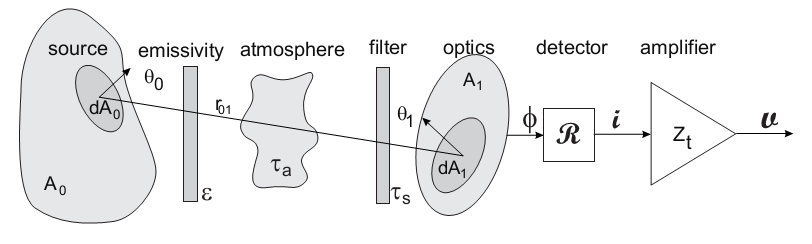
\includegraphics{simplesystem.png}}\hfill}

The amplifier output signal
can be calculated in the following equation,  by integrating  over
all wavelengths, over the full source area \(A_0\) and over the optical
aperture area \(A_1\),
\begin{gather}
\begin{split}v=
Z_t
\int_{A_0}
\int_{A_1}
\frac{1}{r_{01}^2}
\int_0^\infty
\epsilon_\lambda L_\lambda(T,A_0)\tau_{a\lambda}\tau_{s\lambda}(A_1){\cal R}_\lambda
\;d\lambda
\;d(\cos\theta_0 A_0)
\;d(\cos\theta_1 A_1)\end{split}\notag
\end{gather}
where
\(v\) is the output signal voltage,
\(r_{01}\) is the distance between elemental areas
\(d(\cos\theta_0 A_0)\) and
\(d(\cos\theta_1 A_1)\),
\(\epsilon_\lambda\) is the source spectral emissivity,
\(L_\lambda(T,A_0)\) is the Planck Law radiation at temperature
\(T\) at location \(A_0\),
\(\tau_{a\lambda}\) is the atmospheric spectral transmittance,
\(\tau_{s\lambda}(A_1)\) is the sensor spectral transmittance at location \(A_1\),
\({\cal R}_\lambda\) is the spectral detector responsivity in {[}A/W{]},
\(Z_t\) is the amplifier transimpedance gain in {[}V/A{]}.
The spectral integral \(\int_0^\infty d\lambda\) accounts for the total
flux for all wavelengths, the spatial integral
\(\int_{A_0}d(\cos\theta_0 A_0)\)
accounts for flux over the total area of the source, and
the spatial integral
\(\int_{A_1}d(\cos\theta_1 A_1)\) accounts for the total area of the receiving area.

The top graphic in the following figure illustrates the
reasoning behind the spectral integral as a product, followed by an integral (summation),

{\hfill\scalebox{0.500000}{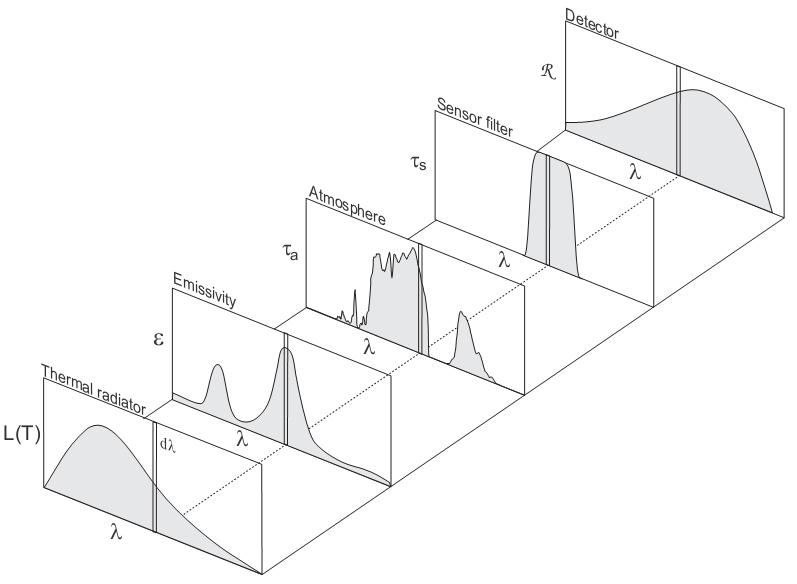
\includegraphics{multispectral.png}}\hfill}
\begin{gather}
\begin{split}\int_0^\infty
\epsilon_\lambda L_\lambda(T)\tau_{a\lambda}\tau_{s\lambda}{\cal R}_\lambda
\;d\lambda,\end{split}\notag
\end{gather}
where the spectral variability of the  source, medium and sensor parameters
are multiplied as spectral variables and afterwards integrated over all wavelengths
to yield the total in-band signal. The domain of spectral quantities can be
stated in terms of a wavelength, wavenumber, or less often, temporal frequency.

Likewise, the source radiance is integrated over the two respective areas of the
target \(A_0\), and the sensor aperture \(A_1\).  Note that if the
sensor field of  view footprint at the source is smaller than the physical
source area, only the flux emanating from the footprint area is integrated.

This example is a relatively complete worked example. The objective is to
calculate the signal of a simple sensor, detecting the presence or absence of
a flame in the sensor field of view. The sensor is pointed to an area just
outside a furnace smokestack, against a clear sky background. The sensor
must detect a change in signal, to indicate the presence or absence of a flame.

The sensor has an aperture area of \(7.8 \times 10^{-3}\) \({\rm m}^2\)
and  a field of view of \(1 \times 10^{-4}\) sr. The sensor filter spectral
transmittance is shown below. The InSb detector has a peak responsivity of 2.5
A/W and normalised spectral response shown below. The preamplifier transimpedance
is 10000 V/A.

The flame area is  1 \({\rm m}^2\), the flame temperature is
\(1000^\circ\) C, and the emissivity is shown below. The emissivity
is 0.1 over most of the spectral band, due to carbon particles in the flame.
At 4.3 \(\mu{\rm m}\) there is a strong emissivity rise due to the hot
carbon dioxide \({\rm CO}_2\) in the flame.

The distance between the flame and the sensor is 1000\textasciitilde{}m. The atmospheric
properties are calculated with the Modtran Tropical climatic model. The
path is oriented such that the sensor stares out to space, at a zenith angle
of \(88^\circ\). The spectral transmittance and path radiance along this
path is shown in below.

The peak in the flame emissivity and the dip in atmospheric transmittance are
both centered around the \(4.3\mu{\rm m}\) \({\rm CO}_2\) band. The calculation
of flux
radiative transfer through the atmosphere must account for the strong spectral
variation, by using a spectral integral.

The signal caused by the flame is given by the equation above, where the
integrals over the surfaces of the flame and sensor are just their respective
areas. The signal caused by the atmospheric path radiance is given by
\begin{gather}
\begin{split}v=
Z_t
\omega_{\rm optics}
A_{\rm optics}
\int_0^\infty
L_{{\rm path}\lambda}
\tau_{s\lambda}{\cal R}_\lambda
\;d\lambda,\end{split}\notag
\end{gather}
where
\(\omega_{\rm optics}\) is the sensor field of view,
\(A_{\rm optics}\) is the optical aperture area,
\(L_{{\rm path}\lambda}\) is the spectral path radiance
and the rest of the symbols are as defined above.

{\hfill\scalebox{0.700000}{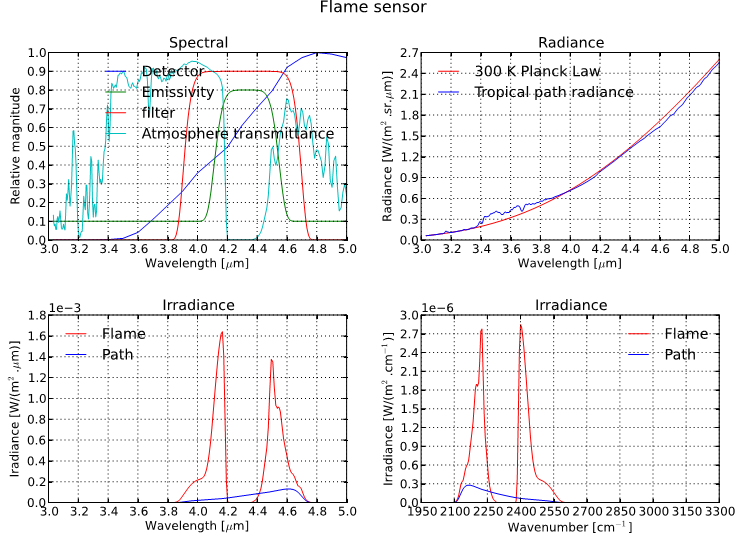
\includegraphics{flamesensor.png}}\hfill}

The pyradi code to model this sensor is available as \href{http://code.google.com/p/pyradi/source/browse/trunk/exflamesensor.py}{exflamesensor.py}.
The output from this script is as follows:

\begin{Verbatim}[commandchars=\\\{\}]
Optics   : area=0.0078 m\PYGZca{}2 FOV=0.0001 [sr]
Amplifier: gain=10000.0 [V/A]
Detector : peak responsivity=2.5 [A/W]
Flame    : temperature=1273.16 [K] area=1 [m\PYGZca{}2] distance=1000 [m] fill=0.01 [\PYGZhy{}]
Flame    : irradiance= 3.29e\PYGZhy{}04 [W/m\PYGZca{}2] signal= 0.0641 [V]
Path     : irradiance= 5.45e\PYGZhy{}05 [W/m\PYGZca{}2] signal= 0.0106 [V]
\end{Verbatim}

It is clear that the flame signal is six times larger than the path radiance
signal, even though the flame fills only 0.01 of the sensor field of view.


\chapter{Planck and thermal radiation}
\label{ryplanck:exflamesensor-py}\label{ryplanck:planck-and-thermal-radiation}\label{ryplanck::doc}

\section{Overview}
\label{ryplanck:overview}\label{ryplanck:module-pyradi.ryplanck}\index{pyradi.ryplanck (module)}
This module provides functions for Planck law exitance calculations, as well as
temperature derivative calculations.
The functions provide spectral exitance in {[}W/(m\textasciicircum{}2.*){]} or {[}q/(s.m\textasciicircum{}2.*){]}, given
the temperature and a vector of one of wavelength, wavenumbers or frequency
(six combinations each for exitance and temperature derivative). The total
exitance can also be calculated by using the Stefan-Boltzman equation, in
{[}W/m\textasciicircum{}2{]} or {[}q/(s.m\textasciicircum{}2){]}.  `Exitance' is the CIE/ISO term for the older term `emittance'.

The Planck and temperature-derivative Planck functions take the spectral variable
(wavelength, wavenumber or frequency) and/or temperature as either a scalar, a 
single element list, a multi-element list or a numpy array.

Spectral values must be strictly scalar or shape (N,) or (N,1).  
Shape (1,N) will not work.

Temperature values must be strictly scalar, list{[}M{]}, shape (M,), (M,1), or (1,M).
Shape (Q,M) will not work.

If the spectral variable and temperature are both single numbers (scalars or lists
with one element), the return value is a scalar.  If either the temperature or the
spectral variable are single-valued, the return value is a rank-1 vector. If both
the temperature and spectral variable are multi-valued, the return value is a 
rank-2 array, with the spectral variable along axis=0.

This module uses the CODATA physical constants. For more details see
\href{http://physics.nist.gov/cuu/pdf/RevModPhysCODATA2010.pdf}{http://physics.nist.gov/cuu/pdf/RevModPhysCODATA2010.pdf}

See the \_\_main\_\_ function for testing and examples of use.

This package was partly developed to provide additional material in support of students 
and readers of the book Electro-Optical System Analysis and Design: A Radiometry 
Perspective,  Cornelius J. Willers, ISBN 9780819495693, SPIE Monograph Volume
PM236, SPIE Press, 2013.  \href{http://spie.org/x648.html?product\_id=2021423\&origin\_id=x646}{http://spie.org/x648.html?product\_id=2021423\&origin\_id=x646}


\section{Module classes}
\label{ryplanck:module-classes}\index{PlanckConstants (class in pyradi.ryplanck)}

\begin{fulllineitems}
\phantomsection\label{ryplanck:pyradi.ryplanck.PlanckConstants}\pysigline{\strong{class }\code{pyradi.ryplanck.}\bfcode{PlanckConstants}}
Precalculate the Planck function constants using the values in
scipy.constants.  Presumbly these constants are up to date and
will be kept up to date.

This module uses the CODATA physical constants. For more details see
\href{http://physics.nist.gov/cuu/pdf/RevModPhysCODATA2010.pdf}{http://physics.nist.gov/cuu/pdf/RevModPhysCODATA2010.pdf}
\begin{quote}

Reference: \href{http://docs.scipy.org/doc/scipy/reference/constants.html}{http://docs.scipy.org/doc/scipy/reference/constants.html}
\end{quote}
\index{printConstants() (pyradi.ryplanck.PlanckConstants method)}

\begin{fulllineitems}
\phantomsection\label{ryplanck:pyradi.ryplanck.PlanckConstants.printConstants}\pysiglinewithargsret{\bfcode{printConstants}}{}{}
Print Planck function constants.
\begin{description}
\item[{Args:}] \leavevmode
\begin{DUlineblock}{0em}
\item[] None
\end{DUlineblock}

\item[{Returns:}] \leavevmode
\begin{DUlineblock}{0em}
\item[] Print to stdout
\end{DUlineblock}

\item[{Raises:}] \leavevmode
\begin{DUlineblock}{0em}
\item[] No exception is raised.
\end{DUlineblock}

\end{description}

\end{fulllineitems}


\end{fulllineitems}



\section{Module functions}
\label{ryplanck:module-functions}\index{planck() (in module pyradi.ryplanck)}

\begin{fulllineitems}
\phantomsection\label{ryplanck:pyradi.ryplanck.planck}\pysiglinewithargsret{\code{pyradi.ryplanck.}\bfcode{planck}}{\emph{spectral}, \emph{temperature}, \emph{type='el'}}{}
Planck law spectral exitance.

Calculates the Planck law spectral exitance from a surface at the stated 
temperature. Temperature can be a scalar, a list or an array. Exitance can 
be given in radiant or photon rate units, depending on user input in type.
\begin{description}
\item[{Args:}] \leavevmode
\begin{DUlineblock}{0em}
\item[] spectral (scalar, np.array (N,) or (N,1)):  spectral vector.
\item[] temperature (scalar, list{[}M{]}, np.array (M,), (M,1) or (1,M)):  Temperature in {[}K{]}
\item[] type (string):
\item[]
\begin{DUlineblock}{\DUlineblockindent}
\item[] `e' signifies Radiant values in {[}W/m\textasciicircum{}2.*{]}.
\item[] `q' signifies photon rate values  {[}quanta/(s.m\textasciicircum{}2.*){]}.
\item[] `l' signifies wavelength spectral vector  {[}micrometer{]}.
\item[] `n' signifies wavenumber spectral vector {[}cm-1{]}.
\item[] `f' signifies frequency spectral vecor {[}Hz{]}.
\end{DUlineblock}
\end{DUlineblock}

\item[{Returns:}] \leavevmode
\begin{DUlineblock}{0em}
\item[] (scalar, np.array{[}N,M{]}):  spectral radiant exitance (not radiance) in units selected.
\item[] For type = `el' units will be {[}W/(m\textasciicircum{}2.um){]}.
\item[] For type = `qf' units will be {[}q/(s.m\textasciicircum{}2.Hz){]}.
\item[] Other return types are similarly defined as above.
\item[] Returns None on error.
\end{DUlineblock}

\item[{Raises:}] \leavevmode
\begin{DUlineblock}{0em}
\item[] No exception is raised, returns None on error.
\end{DUlineblock}

\end{description}

\end{fulllineitems}

\index{dplanck() (in module pyradi.ryplanck)}

\begin{fulllineitems}
\phantomsection\label{ryplanck:pyradi.ryplanck.dplanck}\pysiglinewithargsret{\code{pyradi.ryplanck.}\bfcode{dplanck}}{\emph{spectral}, \emph{temperature}, \emph{type='el'}}{}
Temperature derivative of Planck law exitance.

Calculates the temperature derivative for Planck law spectral exitance
from a surface at the stated temperature. dM/dT can be given in radiant or
photon rate units, depending on user input in type. Temperature can be a 
scalar, a list or an array.
\begin{description}
\item[{Args:}] \leavevmode
\begin{DUlineblock}{0em}
\item[] spectral (scalar, np.array (N,) or (N,1)):  spectral vector in  {[}micrometer{]}, {[}cm-1{]} or {[}Hz{]}.
\item[] temperature (scalar, list{[}M{]}, np.array (M,), (M,1) or (1,M)):  Temperature in {[}K{]}
\item[] type (string):
\item[]
\begin{DUlineblock}{\DUlineblockindent}
\item[] `e' signifies Radiant values in {[}W/(m\textasciicircum{}2.K){]}.
\item[] `q' signifies photon rate values  {[}quanta/(s.m\textasciicircum{}2.K){]}.
\item[] `l' signifies wavelength spectral vector  {[}micrometer{]}.
\item[] `n' signifies wavenumber spectral vector {[}cm-1{]}.
\item[] `f' signifies frequency spectral vecor {[}Hz{]}.
\end{DUlineblock}
\end{DUlineblock}

\item[{Returns:}] \leavevmode
\begin{DUlineblock}{0em}
\item[] (scalar, np.array{[}N,M{]}):  spectral radiant exitance (not radiance) in units selected.
\item[] For type = `el' units will be {[}W/(m2.um.K){]}
\item[] For type = `qf' units will be {[}q/(s.m2.Hz.K){]}
\item[] Other return types are similarly defined as above.
\item[] Returns None on error.
\end{DUlineblock}

\item[{Raises:}] \leavevmode
\begin{DUlineblock}{0em}
\item[] No exception is raised, returns None on error.
\end{DUlineblock}

\end{description}

\end{fulllineitems}

\index{stefanboltzman() (in module pyradi.ryplanck)}

\begin{fulllineitems}
\phantomsection\label{ryplanck:pyradi.ryplanck.stefanboltzman}\pysiglinewithargsret{\code{pyradi.ryplanck.}\bfcode{stefanboltzman}}{\emph{temperature}, \emph{type='e'}}{}
Stefan-Boltzman wideband integrated exitance.

Calculates the total Planck law exitance, integrated over all wavelengths,
from a surface at the stated temperature. Exitance can be given in radiant or
photon rate units, depending on user input in type.
\begin{description}
\item[{Args:}] \leavevmode
\begin{DUlineblock}{0em}
\item[] (scalar, list{[}M{]}, np.array (M,), (M,1) or (1,M)):  Temperature in {[}K{]}
\item[] type (string):  `e' for radiant or `q' for photon rate exitance.
\end{DUlineblock}

\item[{Returns:}] \leavevmode
\begin{DUlineblock}{0em}
\item[] (float): integrated radiant exitance in  {[}W/m\textasciicircum{}2{]} or {[}q/(s.m\textasciicircum{}2){]}.
\item[] Returns a -1 if the type is not `e' or `q'
\end{DUlineblock}

\item[{Raises:}] \leavevmode
\begin{DUlineblock}{0em}
\item[] No exception is raised.
\end{DUlineblock}

\end{description}

\end{fulllineitems}

\index{planckel() (in module pyradi.ryplanck)}

\begin{fulllineitems}
\phantomsection\label{ryplanck:pyradi.ryplanck.planckel}\pysiglinewithargsret{\code{pyradi.ryplanck.}\bfcode{planckel}}{\emph{spectral}, \emph{temperature}}{}
Planck function in wavelength for radiant exitance.
\begin{description}
\item[{Args:}] \leavevmode
\begin{DUlineblock}{0em}
\item[] spectral (scalar, np.array (N,) or (N,1)):  wavelength vector in  {[}um{]}
\item[] temperature (scalar, list{[}M{]}, np.array (M,), (M,1) or (1,M)):  Temperature in {[}K{]}
\end{DUlineblock}

\item[{Returns:}] \leavevmode
\begin{DUlineblock}{0em}
\item[] (scalar, np.array{[}N,M{]}):  spectral radiant exitance in W/(m\textasciicircum{}2.um)
\end{DUlineblock}

\item[{Raises:}] \leavevmode
\begin{DUlineblock}{0em}
\item[] No exception is raised, returns None on error.
\end{DUlineblock}

\end{description}

\end{fulllineitems}

\index{plancken() (in module pyradi.ryplanck)}

\begin{fulllineitems}
\phantomsection\label{ryplanck:pyradi.ryplanck.plancken}\pysiglinewithargsret{\code{pyradi.ryplanck.}\bfcode{plancken}}{\emph{spectral}, \emph{temperature}}{}
Planck function in wavenumber for radiant exitance.
\begin{description}
\item[{Args:}] \leavevmode
\begin{DUlineblock}{0em}
\item[] spectral (scalar, np.array (N,) or (N,1)):  wavenumber vector in   {[}cm\textasciicircum{}-1{]}
\item[] temperature (scalar, list{[}M{]}, np.array (M,), (M,1) or (1,M)):  Temperature in {[}K{]}
\end{DUlineblock}

\item[{Returns:}] \leavevmode
\begin{DUlineblock}{0em}
\item[] (scalar, np.array{[}N,M{]}):  spectral radiant exitance in  W/(m\textasciicircum{}2.cm\textasciicircum{}-1)
\end{DUlineblock}

\item[{Raises:}] \leavevmode
\begin{DUlineblock}{0em}
\item[] No exception is raised, returns None on error.
\end{DUlineblock}

\end{description}

\end{fulllineitems}

\index{planckef() (in module pyradi.ryplanck)}

\begin{fulllineitems}
\phantomsection\label{ryplanck:pyradi.ryplanck.planckef}\pysiglinewithargsret{\code{pyradi.ryplanck.}\bfcode{planckef}}{\emph{spectral}, \emph{temperature}}{}
Planck function in frequency for radiant exitance.
\begin{description}
\item[{Args:}] \leavevmode
\begin{DUlineblock}{0em}
\item[] spectral (scalar, np.array (N,) or (N,1)):  frequency vector in  {[}Hz{]}
\item[] temperature (scalar, list{[}M{]}, np.array (M,), (M,1) or (1,M)):  Temperature in {[}K{]}
\end{DUlineblock}

\item[{Returns:}] \leavevmode
\begin{DUlineblock}{0em}
\item[] (scalar, np.array{[}N,M{]}): spectral radiant exitance in W/(m\textasciicircum{}2.Hz)
\end{DUlineblock}

\item[{Raises:}] \leavevmode
\begin{DUlineblock}{0em}
\item[] No exception is raised, returns None on error.
\end{DUlineblock}

\end{description}

\end{fulllineitems}

\index{planckql() (in module pyradi.ryplanck)}

\begin{fulllineitems}
\phantomsection\label{ryplanck:pyradi.ryplanck.planckql}\pysiglinewithargsret{\code{pyradi.ryplanck.}\bfcode{planckql}}{\emph{spectral}, \emph{temperature}}{}
Planck function in wavelength domain for photon rate exitance.
\begin{description}
\item[{Args:}] \leavevmode
\begin{DUlineblock}{0em}
\item[] spectral (scalar, np.array (N,) or (N,1)):  wavelength vector in  {[}um{]}
\item[] temperature (scalar, list{[}M{]}, np.array (M,), (M,1) or (1,M)):  Temperature in {[}K{]}
\end{DUlineblock}

\item[{Returns:}] \leavevmode
\begin{DUlineblock}{0em}
\item[] (scalar, np.array{[}N,M{]}):  spectral radiant exitance in  q/(s.m\textasciicircum{}2.um)
\end{DUlineblock}

\item[{Raises:}] \leavevmode
\begin{DUlineblock}{0em}
\item[] No exception is raised, returns None on error.
\end{DUlineblock}

\end{description}

\end{fulllineitems}

\index{planckqn() (in module pyradi.ryplanck)}

\begin{fulllineitems}
\phantomsection\label{ryplanck:pyradi.ryplanck.planckqn}\pysiglinewithargsret{\code{pyradi.ryplanck.}\bfcode{planckqn}}{\emph{spectral}, \emph{temperature}}{}
Planck function in wavenumber domain for photon rate exitance.
\begin{description}
\item[{Args:}] \leavevmode
\begin{DUlineblock}{0em}
\item[] spectral (scalar, np.array (N,) or (N,1)):  wavenumber vector in   {[}cm\textasciicircum{}-1{]}
\item[] temperature (scalar, list{[}M{]}, np.array (M,), (M,1) or (1,M)):  Temperature in {[}K{]}
\end{DUlineblock}

\item[{Returns:}] \leavevmode
\begin{DUlineblock}{0em}
\item[] (scalar, np.array{[}N,M{]}):  spectral radiant exitance in  q/(s.m\textasciicircum{}2.cm\textasciicircum{}-1)
\end{DUlineblock}

\item[{Raises:}] \leavevmode
\begin{DUlineblock}{0em}
\item[] No exception is raised, returns None on error.
\end{DUlineblock}

\end{description}

\end{fulllineitems}

\index{planckqf() (in module pyradi.ryplanck)}

\begin{fulllineitems}
\phantomsection\label{ryplanck:pyradi.ryplanck.planckqf}\pysiglinewithargsret{\code{pyradi.ryplanck.}\bfcode{planckqf}}{\emph{spectral}, \emph{temperature}}{}
Planck function in frequency domain for photon rate exitance.
\begin{description}
\item[{Args:}] \leavevmode
\begin{DUlineblock}{0em}
\item[] spectral (scalar, np.array (N,) or (N,1)): frequency vector in  {[}Hz{]}
\item[] temperature (scalar, list{[}M{]}, np.array (M,), (M,1) or (1,M)):  Temperature in {[}K{]}
\end{DUlineblock}

\item[{Returns:}] \leavevmode
\begin{DUlineblock}{0em}
\item[] (scalar, np.array{[}N,M{]}):  spectral radiant exitance in q/(s.m\textasciicircum{}2.Hz)
\end{DUlineblock}

\item[{Raises:}] \leavevmode
\begin{DUlineblock}{0em}
\item[] No exception is raised, returns None on error.
\end{DUlineblock}

\end{description}

\end{fulllineitems}

\index{dplnckel() (in module pyradi.ryplanck)}

\begin{fulllineitems}
\phantomsection\label{ryplanck:pyradi.ryplanck.dplnckel}\pysiglinewithargsret{\code{pyradi.ryplanck.}\bfcode{dplnckel}}{\emph{spectral}, \emph{temperature}}{}
Temperature derivative of Planck function in wavelength domain for
radiant exitance.
\begin{description}
\item[{Args:}] \leavevmode
\begin{DUlineblock}{0em}
\item[] spectral (scalar, np.array (N,) or (N,1)):  wavelength vector in  {[}um{]}
\item[] temperature (scalar, list{[}M{]}, np.array (M,), (M,1) or (1,M)):  Temperature in {[}K{]}
\end{DUlineblock}

\item[{Returns:}] \leavevmode
\begin{DUlineblock}{0em}
\item[] (scalar, np.array{[}N,M{]}):  spectral radiant exitance in W/(K.m\textasciicircum{}2.um)
\end{DUlineblock}

\item[{Raises:}] \leavevmode
\begin{DUlineblock}{0em}
\item[] No exception is raised, returns None on error.
\end{DUlineblock}

\end{description}

\end{fulllineitems}

\index{dplncken() (in module pyradi.ryplanck)}

\begin{fulllineitems}
\phantomsection\label{ryplanck:pyradi.ryplanck.dplncken}\pysiglinewithargsret{\code{pyradi.ryplanck.}\bfcode{dplncken}}{\emph{spectral}, \emph{temperature}}{}
Temperature derivative of Planck function in wavenumber domain for radiance exitance.
\begin{description}
\item[{Args:}] \leavevmode
\begin{DUlineblock}{0em}
\item[] spectral (scalar, np.array (N,) or (N,1)):  wavenumber vector in   {[}cm\textasciicircum{}-1{]}
\item[] temperature (scalar, list{[}M{]}, np.array (M,), (M,1) or (1,M)):  Temperature in {[}K{]}
\end{DUlineblock}

\item[{Returns:}] \leavevmode
\begin{DUlineblock}{0em}
\item[] (scalar, np.array{[}N,M{]}):  spectral radiant exitance in  W/(K.m\textasciicircum{}2.cm\textasciicircum{}-1)
\end{DUlineblock}

\item[{Raises:}] \leavevmode
\begin{DUlineblock}{0em}
\item[] No exception is raised, returns None on error.
\end{DUlineblock}

\end{description}

\end{fulllineitems}

\index{dplnckef() (in module pyradi.ryplanck)}

\begin{fulllineitems}
\phantomsection\label{ryplanck:pyradi.ryplanck.dplnckef}\pysiglinewithargsret{\code{pyradi.ryplanck.}\bfcode{dplnckef}}{\emph{spectral}, \emph{temperature}}{}
Temperature derivative of Planck function in frequency domain
for radiant exitance.
\begin{description}
\item[{Args:}] \leavevmode
\begin{DUlineblock}{0em}
\item[] spectral (scalar, np.array (N,) or (N,1)): frequency vector in  {[}Hz{]}
\item[] temperature (scalar, list{[}M{]}, np.array (M,), (M,1) or (1,M)):  Temperature in {[}K{]}
\end{DUlineblock}

\item[{Returns:}] \leavevmode
\begin{DUlineblock}{0em}
\item[] (scalar, np.array{[}N,M{]}):  spectral radiant exitance/K in W/(K.m\textasciicircum{}2.Hz)
\end{DUlineblock}

\item[{Raises:}] \leavevmode
\begin{DUlineblock}{0em}
\item[] No exception is raised, returns None on error.
\end{DUlineblock}

\end{description}

\end{fulllineitems}

\index{dplnckql() (in module pyradi.ryplanck)}

\begin{fulllineitems}
\phantomsection\label{ryplanck:pyradi.ryplanck.dplnckql}\pysiglinewithargsret{\code{pyradi.ryplanck.}\bfcode{dplnckql}}{\emph{spectral}, \emph{temperature}}{}
Temperature derivative of Planck function in wavenumber domain for radiance exitance.
\begin{description}
\item[{Args:}] \leavevmode
\begin{DUlineblock}{0em}
\item[] spectral (scalar, np.array (N,) or (N,1)):  wavelength vector in  {[}um{]}
\item[] temperature (scalar, list{[}M{]}, np.array (M,), (M,1) or (1,M)):  Temperature in {[}K{]}
\end{DUlineblock}

\item[{Returns:}] \leavevmode
\begin{DUlineblock}{0em}
\item[] (scalar, np.array{[}N,M{]}):  spectral radiant exitance in  q/(K.s.m\textasciicircum{}2.um)
\end{DUlineblock}

\item[{Raises:}] \leavevmode
\begin{DUlineblock}{0em}
\item[] No exception is raised, returns None on error.
\end{DUlineblock}

\end{description}

\end{fulllineitems}

\index{dplnckqn() (in module pyradi.ryplanck)}

\begin{fulllineitems}
\phantomsection\label{ryplanck:pyradi.ryplanck.dplnckqn}\pysiglinewithargsret{\code{pyradi.ryplanck.}\bfcode{dplnckqn}}{\emph{spectral}, \emph{temperature}}{}
Temperature derivative of Planck function in wavenumber domain for photon rate.
\begin{description}
\item[{Args:}] \leavevmode
\begin{DUlineblock}{0em}
\item[] spectral (scalar, np.array (N,) or (N,1)):  wavenumber vector in   {[}cm\textasciicircum{}-1{]}
\item[] temperature (scalar, list{[}M{]}, np.array (M,), (M,1) or (1,M)):  Temperature in {[}K{]}
\end{DUlineblock}

\item[{Returns:}] \leavevmode
\begin{DUlineblock}{0em}
\item[] (scalar, np.array{[}N,M{]}):  spectral radiant exitance in  q/(s.m\textasciicircum{}2.cm\textasciicircum{}-1)
\end{DUlineblock}

\item[{Raises:}] \leavevmode
\begin{DUlineblock}{0em}
\item[] No exception is raised, returns None on error.
\end{DUlineblock}

\end{description}

\end{fulllineitems}

\index{dplnckqf() (in module pyradi.ryplanck)}

\begin{fulllineitems}
\phantomsection\label{ryplanck:pyradi.ryplanck.dplnckqf}\pysiglinewithargsret{\code{pyradi.ryplanck.}\bfcode{dplnckqf}}{\emph{spectral}, \emph{temperature}}{}
Temperature derivative of Planck function in frequency domain for photon rate.
\begin{description}
\item[{Args:}] \leavevmode
\begin{DUlineblock}{0em}
\item[] spectral (scalar, np.array (N,) or (N,1)): frequency vector in  {[}Hz{]}
\item[] temperature (scalar, list{[}M{]}, np.array (M,), (M,1) or (1,M)):  Temperature in {[}K{]}
\end{DUlineblock}

\item[{Returns:}] \leavevmode
\begin{DUlineblock}{0em}
\item[] (scalar, np.array{[}N,M{]}):  spectral radiant exitance in q/(K.s.m\textasciicircum{}2.Hz)
\end{DUlineblock}

\item[{Raises:}] \leavevmode
\begin{DUlineblock}{0em}
\item[] No exception is raised, returns None on error.
\end{DUlineblock}

\end{description}

\end{fulllineitems}



\chapter{File reading/writing utility}
\label{ryfiles:file-reading-writing-utility}\label{ryfiles::doc}

\section{Overview}
\label{ryfiles:module-pyradi.ryfiles}\label{ryfiles:overview}\index{pyradi.ryfiles (module)}
This module provides functions for file input/output. These are all wrapper
functions, based on existing functions in other Python classes. Functions are 
provided to save a two-dimensional array to a text file, load selected columns 
of data from a text file, load a column header line, compact strings to include 
only legal filename characters, and a function from the Python Cookbook to 
recursively match filename patterns.

See the \_\_main\_\_ function for examples of use.

This package was partly developed to provide additional material in support of students 
and readers of the book Electro-Optical System Analysis and Design: A Radiometry 
Perspective,  Cornelius J. Willers, ISBN 9780819495693, SPIE Monograph Volume
PM236, SPIE Press, 2013.  \href{http://spie.org/x648.html?product\_id=2021423\&origin\_id=x646}{http://spie.org/x648.html?product\_id=2021423\&origin\_id=x646}


\section{Module functions}
\label{ryfiles:module-functions}\index{saveHeaderArrayTextFile() (in module pyradi.ryfiles)}

\begin{fulllineitems}
\phantomsection\label{ryfiles:pyradi.ryfiles.saveHeaderArrayTextFile}\pysiglinewithargsret{\code{pyradi.ryfiles.}\bfcode{saveHeaderArrayTextFile}}{\emph{filename}, \emph{dataArray}, \emph{header=None}, \emph{comment=None}, \emph{delimiter=None}}{}
Save a numpy array to a file, included header lines.

This function saves a two-dimensional array to a text file, with
an optional user-defined header. This functionality will be part of
numpy 1.7, when released.
\begin{description}
\item[{Args:}] \leavevmode
\begin{DUlineblock}{0em}
\item[] filename (string): name of the output ASCII flatfile.
\item[] dataArray (np.array{[}N,M{]}): a two-dimensional array.
\item[] header (string): the optional header.
\item[] comment (string): the symbol used to comment out lines, default value is None.
\item[] delimiter (string): delimiter used to separate columns, default is whitespace.
\end{DUlineblock}

\item[{Returns:}] \leavevmode
\begin{DUlineblock}{0em}
\item[] Nothing.
\end{DUlineblock}

\item[{Raises:}] \leavevmode
\begin{DUlineblock}{0em}
\item[] No exception is raised.
\end{DUlineblock}

\end{description}

\end{fulllineitems}

\index{loadColumnTextFile() (in module pyradi.ryfiles)}

\begin{fulllineitems}
\phantomsection\label{ryfiles:pyradi.ryfiles.loadColumnTextFile}\pysiglinewithargsret{\code{pyradi.ryfiles.}\bfcode{loadColumnTextFile}}{\emph{filename, loadCol={[}1{]}, comment=None, normalize=0, skiprows=0, delimiter=None, abscissaScale=1, ordinateScale=1, abscissaOut=None, returnAbscissa=False}}{}
Load selected column data from a text file, processing as specified.

This function loads column data from a text file, scaling and interpolating 
the read-in data, according to user specification. The first 0'th column has 
special significance: it is considered the abscissa (x-values) of the data 
set, while the remaining columns are any number of ordinate (y-value) vectors.
The user passes a list of columns to be read (default is {[}1{]}) - only these 
columns are read, processed and returned when the function exits.The user 
also passes an abscissa vector to which the input data is interpolated and 
then subsequently amplitude scaled or normalised.

Note: leave only single separators (e.g. spaces) between columns!
Also watch out for a single space at the start of line.
\begin{description}
\item[{Args:}] \leavevmode
\begin{DUlineblock}{0em}
\item[] filename (string): name of the input ASCII flatfile.
\item[] loadCol ({[}int{]}): the M =len({[}{]}) column(s) to be loaded as the ordinate, default value is column 1
\item[] comment (string): string, the symbol used to comment out lines, default value is None
\item[] normalize (int): integer, flag to indicate if data must be normalized.
\item[] skiprows (int): integer, the number of rows to be skipped at the start of the file (e.g. headers)
\item[] delimiter (string): string, the delimiter used to separate columns, default is whitespace.
\item[] abscissaScale (float): scale by which abscissa (column 0) must be multiplied
\item[] ordinateScale (float): scale by which ordinate (column \textgreater{}0) must be multiplied
\item[] abscissaOut (np.array{[}N,{]} or {[}N,1{]}): abscissa vector on which output variables are interpolated.
\item[] returnAbscissa (bool): return the abscissa vector as second item in return tuple.
\end{DUlineblock}

\item[{Returns:}] \leavevmode
\begin{DUlineblock}{0em}
\item[] ordinatesOut (np.array{[}N,M{]}): The interpolated, M columns of N rows, processed array.
\item[] abscissaOut (np.array{[}N,M{]}): The ascissa where the ordinates are interpolated
\end{DUlineblock}

\item[{Raises:}] \leavevmode
\begin{DUlineblock}{0em}
\item[] No exception is raised.
\end{DUlineblock}

\end{description}

\end{fulllineitems}

\index{loadHeaderTextFile() (in module pyradi.ryfiles)}

\begin{fulllineitems}
\phantomsection\label{ryfiles:pyradi.ryfiles.loadHeaderTextFile}\pysiglinewithargsret{\code{pyradi.ryfiles.}\bfcode{loadHeaderTextFile}}{\emph{filename, loadCol={[}1{]}, comment=None}}{}
Loads column header data in the first string of a text file.

loads column header data from a file, from the first row.
Headers must be delimited by commas. The function {[}LoadColumnTextFile{]} provides
more comprehensive capabilties.
\begin{description}
\item[{Args:}] \leavevmode
\begin{DUlineblock}{0em}
\item[] filename (string): the name of the input ASCII flatfile.
\item[] loadCol ({[}int{]}): list of numbers, the column headers to be loaded , default value is column 1
\item[] comment (string): the symbol to comment out lines
\end{DUlineblock}

\item[{Returns:}] \leavevmode
\begin{DUlineblock}{0em}
\item[] {[}string{]}: a list with selected column header entries
\end{DUlineblock}

\item[{Raises:}] \leavevmode
\begin{DUlineblock}{0em}
\item[] No exception is raised.
\end{DUlineblock}

\end{description}

\end{fulllineitems}

\index{cleanFilename() (in module pyradi.ryfiles)}

\begin{fulllineitems}
\phantomsection\label{ryfiles:pyradi.ryfiles.cleanFilename}\pysiglinewithargsret{\code{pyradi.ryfiles.}\bfcode{cleanFilename}}{\emph{sourcestring}, \emph{removestring=u' \%:/}, \emph{.\textbackslash{}\textbackslash{}{[}{]}'}}{}
Clean a string by removing selected characters.

Creates a legal and `clean' source string from a string by removing some 
clutter and  characters not allowed in filenames.
A default set is given but the user can override the default string.
\begin{description}
\item[{Args:}] \leavevmode
\begin{DUlineblock}{0em}
\item[] sourcestring (string): the string to be cleaned.
\item[] removestring (string): remove all these characters from the string (optional).
\end{DUlineblock}

\item[{Returns:}] \leavevmode
\begin{DUlineblock}{0em}
\item[] (string): A cleaned-up string.
\end{DUlineblock}

\item[{Raises:}] \leavevmode
\begin{DUlineblock}{0em}
\item[] No exception is raised.
\end{DUlineblock}

\end{description}

\end{fulllineitems}

\index{listFiles() (in module pyradi.ryfiles)}

\begin{fulllineitems}
\phantomsection\label{ryfiles:pyradi.ryfiles.listFiles}\pysiglinewithargsret{\code{pyradi.ryfiles.}\bfcode{listFiles}}{\emph{root}, \emph{patterns=u'*'}, \emph{recurse=1}, \emph{return\_folders=0}, \emph{useRegex=False}}{}
Lists the files/directories meeting specific requirement
\begin{quote}

Returns a list of file paths to files in a file system, searching a 
directory structure along the specified path, looking for files 
that matches the glob pattern. If specified, the search will continue 
into sub-directories.  A list of matching names is returned. The 
function supports a local or network reachable filesystem, but not URLs.
\end{quote}
\begin{description}
\item[{Args:}] \leavevmode
\begin{DUlineblock}{0em}
\item[] root (string): directory root from where the search must take place
\item[] patterns (string): glob/regex pattern for filename matching
\item[] recurse (unt): flag to indicate if subdirectories must also be searched (optional)
\item[] return\_folders (int): flag to indicate if folder names must also be returned (optional)
\item[] useRegex (bool): flag to indicate if patterns areregular expression strings (optional)
\end{DUlineblock}

\item[{Returns:}] \leavevmode
\begin{DUlineblock}{0em}
\item[] A list with matching file/directory names
\end{DUlineblock}

\item[{Raises:}] \leavevmode
\begin{DUlineblock}{0em}
\item[] No exception is raised.
\end{DUlineblock}

\end{description}

\end{fulllineitems}

\index{readRawFrames() (in module pyradi.ryfiles)}

\begin{fulllineitems}
\phantomsection\label{ryfiles:pyradi.ryfiles.readRawFrames}\pysiglinewithargsret{\code{pyradi.ryfiles.}\bfcode{readRawFrames}}{\emph{fname}, \emph{rows}, \emph{cols}, \emph{vartype}, \emph{loadFrames=}\optional{}}{}
Loading multi-frame two-dimensional arrays from a raw data file of known data type.
\begin{quote}

The file must consist of multiple frames, all with the same number of rows and columns.
Frames of different data types can be read, according to the user specification.  
The user can specify which frames must be loaded (if not the whole file).
\end{quote}
\begin{description}
\item[{Args:}] \leavevmode
\begin{DUlineblock}{0em}
\item[] fname (string): filename
\item[] rows (int): number of rows in each frame
\item[] cols (int): number of columns in each frame
\item[] vartype (np.dtype): numpy data type of data to be read
\item[]
\begin{DUlineblock}{\DUlineblockindent}
\item[] int8, int16, int32, int64
\item[] uint8, uint16, uint32, uint64
\item[] float16, float32, float64
\end{DUlineblock}
\item[] loadFrames ({[}int{]}): optional list of frames to load, zero-based , empty list (default) loads all frames
\end{DUlineblock}

\item[{Returns:}] \leavevmode
\begin{DUlineblock}{0em}
\item[] frames (int) : number of frames in the returned data set,
\item[]
\begin{DUlineblock}{\DUlineblockindent}
\item[] 0 if error occurred
\end{DUlineblock}
\item[] rawShaped (np.ndarray): vartype numpy array of dimensions (frames,rows,cols),
\item[]
\begin{DUlineblock}{\DUlineblockindent}
\item[] None if error occurred
\end{DUlineblock}
\end{DUlineblock}

\item[{Raises:}] \leavevmode
\begin{DUlineblock}{0em}
\item[] No exception is raised.
\end{DUlineblock}

\end{description}

\end{fulllineitems}

\index{rawFrameToImageFile() (in module pyradi.ryfiles)}

\begin{fulllineitems}
\phantomsection\label{ryfiles:pyradi.ryfiles.rawFrameToImageFile}\pysiglinewithargsret{\code{pyradi.ryfiles.}\bfcode{rawFrameToImageFile}}{\emph{image}, \emph{filename}}{}
Writes a single raw image frame to image file.
The file type must be given, e.g. png or jpg.
The image need not be scaled beforehand, it is done prior 
to writing out the image. Could be one of
BMP, JPG, JPEG, PNG, PPM, TIFF, XBM, XPM)
but the file types available depends
on the QT imsave plugin in use.
\begin{description}
\item[{Args:}] \leavevmode
\begin{DUlineblock}{0em}
\item[] image (np.ndarray): two-dimensional array representing an image
\item[] filename (string): name of file to be written to, with extension
\end{DUlineblock}

\item[{Returns:}] \leavevmode
\begin{DUlineblock}{0em}
\item[] Nothing
\end{DUlineblock}

\item[{Raises:}] \leavevmode
\begin{DUlineblock}{0em}
\item[] No exception is raised.
\end{DUlineblock}

\end{description}

\end{fulllineitems}

\index{arrayToLaTex() (in module pyradi.ryfiles)}

\begin{fulllineitems}
\phantomsection\label{ryfiles:pyradi.ryfiles.arrayToLaTex}\pysiglinewithargsret{\code{pyradi.ryfiles.}\bfcode{arrayToLaTex}}{\emph{filename}, \emph{arr}, \emph{header=None}, \emph{leftCol=None}, \emph{formatstring=u'\%1.4e'}, \emph{filemode=u'wt'}}{}
Write a numpy array to latex table format in output file.
\begin{quote}

The table can contain only the array data (no top header or
left column side-header), or you can add either or both of the
top row or side column headers. Leave `header' or `leftcol' as
None is you don't want these.

The output format of the array data can be specified, i.e.
scientific notation or fixed decimal point.
\end{quote}
\begin{description}
\item[{Args:}] \leavevmode
\begin{DUlineblock}{0em}
\item[] fname (string): text writing output path and filename
\item[] arr (np.array{[}N,M{]}): array with table data
\item[] header (string): column header in final latex format (optional)
\item[] leftCol ({[}string{]}): left column each row, in final latex format (optional)
\item[] formatstring (string): output format precision for array data (see np.savetxt) (optional)
\item[] filemode (string): file open mode (a=append, w=new file) (optional)
\end{DUlineblock}

\item[{Returns:}] \leavevmode
\begin{DUlineblock}{0em}
\item[] None, writes a file to disk
\end{DUlineblock}

\item[{Raises:}] \leavevmode
\begin{DUlineblock}{0em}
\item[] No exception is raised.
\end{DUlineblock}

\end{description}

\end{fulllineitems}

\index{epsLaTexFigure() (in module pyradi.ryfiles)}

\begin{fulllineitems}
\phantomsection\label{ryfiles:pyradi.ryfiles.epsLaTexFigure}\pysiglinewithargsret{\code{pyradi.ryfiles.}\bfcode{epsLaTexFigure}}{\emph{filename}, \emph{epsname}, \emph{caption}, \emph{scale}, \emph{filemode=u'a'}}{}~\begin{description}
\item[{Write the LaTeX code to include an eps graphic as a latex figure.}] \leavevmode
The text is added to an existing file.

\item[{Args:}] \leavevmode
\begin{DUlineblock}{0em}
\item[] fname (string):  text writing output path and filename.
\item[] epsname (string): filename/path to eps file (relative to where the LaTeX document is built).
\item[] caption (string): figure caption
\item[] scale (double): figure scale to textwidth {[}0..1{]}
\item[] filemode (string): file open mode (a=append, w=new file) (optional)
\end{DUlineblock}

\item[{Returns:}] \leavevmode
\begin{DUlineblock}{0em}
\item[] None, writes a file to disk
\end{DUlineblock}

\item[{Raises:}] \leavevmode
\begin{DUlineblock}{0em}
\item[] No exception is raised.
\end{DUlineblock}

\end{description}

\end{fulllineitems}

\index{read2DLookupTable() (in module pyradi.ryfiles)}

\begin{fulllineitems}
\phantomsection\label{ryfiles:pyradi.ryfiles.read2DLookupTable}\pysiglinewithargsret{\code{pyradi.ryfiles.}\bfcode{read2DLookupTable}}{\emph{filename}}{}
Read a 2D lookup table and extract the data.
\begin{quote}

The table has the following format:

\begin{Verbatim}[commandchars=\\\{\}]
line 1: xlabel ylabel title
line 2: 0 (vector of y (col) abscissa)
lines 3 and following: (element of x (row) abscissa), followed
by table data.
\end{Verbatim}

From line/row 3 onwards the first element is the x abscissa value
followed by the row of data, one point for each y abscissa value.

The file format can depicted as follows:

\begin{Verbatim}[commandchars=\\\{\}]
x\PYGZhy{}name y\PYGZhy{}name ordinates\PYGZhy{}name
0 y1 y2 y3 y4
x1 v11 v12 v13 v14
x2 v21 v22 v23 v24
x3 v31 v32 v33 v34
x4 v41 v42 v43 v44
x5 v51 v52 v53 v54
x6 v61 v62 v63 v64
\end{Verbatim}

This function reads the file and returns the individual data items.
\end{quote}
\begin{description}
\item[{Args:}] \leavevmode
\begin{DUlineblock}{0em}
\item[] fname (string): input path and filename
\end{DUlineblock}

\item[{Returns:}] \leavevmode
\begin{DUlineblock}{0em}
\item[] xVec ((np.array{[}N{]})): x abscissae
\item[] yVec ((np.array{[}M{]})): y abscissae
\item[] data ((np.array{[}N,M{]})): data corresponding the x,y
\item[] xlabel (string): x abscissa label
\item[] ylabel (string): y abscissa label
\item[] title (string): dataset title
\end{DUlineblock}

\item[{Raises:}] \leavevmode
\begin{DUlineblock}{0em}
\item[] No exception is raised.
\end{DUlineblock}

\end{description}

\end{fulllineitems}

\index{downloadFileUrl() (in module pyradi.ryfiles)}

\begin{fulllineitems}
\phantomsection\label{ryfiles:pyradi.ryfiles.downloadFileUrl}\pysiglinewithargsret{\code{pyradi.ryfiles.}\bfcode{downloadFileUrl}}{\emph{url}, \emph{saveFilename=None}}{}
Download a file, given a URL.

The URL is used to download a file, to the saveFilename specified.
If no saveFilename is given, the basename of the URL is used.
\begin{description}
\item[{Args:}] \leavevmode
\begin{DUlineblock}{0em}
\item[] url (string): the url to be accessed.
\item[] saveFilename (string): path to where the file must be saved (optional).
\end{DUlineblock}

\item[{Returns:}] \leavevmode
\begin{DUlineblock}{0em}
\item[] (string): Filename saved, or None if failed.
\end{DUlineblock}

\item[{Raises:}] \leavevmode
\begin{DUlineblock}{0em}
\item[] Exceptions are handled internally and signaled by return value.
\end{DUlineblock}

\end{description}

\end{fulllineitems}

\index{unzipGZipfile() (in module pyradi.ryfiles)}

\begin{fulllineitems}
\phantomsection\label{ryfiles:pyradi.ryfiles.unzipGZipfile}\pysiglinewithargsret{\code{pyradi.ryfiles.}\bfcode{unzipGZipfile}}{\emph{zipfilename}, \emph{saveFilename=None}}{}
Unzip a file that was compressed using the gzip format.

The zipfilename is used to open a file, to the saveFilename specified.
If no saveFilename is given, the basename of the zipfilename is used, 
but with the file extension removed.
\begin{description}
\item[{Args:}] \leavevmode
\begin{DUlineblock}{0em}
\item[] zipfilename (string): the zipfilename to be decompressed.
\item[] saveFilename (string): to where the file must be saved (optional).
\end{DUlineblock}

\item[{Returns:}] \leavevmode
\begin{DUlineblock}{0em}
\item[] (string): Filename saved, or None if failed.
\end{DUlineblock}

\item[{Raises:}] \leavevmode
\begin{DUlineblock}{0em}
\item[] Exceptions are handled internally and signaled by return value.
\end{DUlineblock}

\end{description}

\end{fulllineitems}

\index{untarTarfile() (in module pyradi.ryfiles)}

\begin{fulllineitems}
\phantomsection\label{ryfiles:pyradi.ryfiles.untarTarfile}\pysiglinewithargsret{\code{pyradi.ryfiles.}\bfcode{untarTarfile}}{\emph{tarfilename}, \emph{saveDirname=None}}{}
Untar a tar archive, and save all files to the specified directory.

The tarfilename is used to open a file, extraxting to the saveDirname specified.
If no saveDirname is given, the local directory `.' is used.
\begin{description}
\item[{Args:}] \leavevmode
\begin{DUlineblock}{0em}
\item[] tarfilename (string): the name of the tar archive.
\item[] saveDirname (string): to where the files must be extracted
\end{DUlineblock}

\item[{Returns:}] \leavevmode
\begin{DUlineblock}{0em}
\item[] ({[}string{]}): list of filenames saved, or None if failed.
\end{DUlineblock}

\item[{Raises:}] \leavevmode
\begin{DUlineblock}{0em}
\item[] Exceptions are handled internally and signaled by return value.
\end{DUlineblock}

\end{description}

\end{fulllineitems}

\index{downloadUntar() (in module pyradi.ryfiles)}

\begin{fulllineitems}
\phantomsection\label{ryfiles:pyradi.ryfiles.downloadUntar}\pysiglinewithargsret{\code{pyradi.ryfiles.}\bfcode{downloadUntar}}{\emph{tgzFilename}, \emph{url}, \emph{destinationDir=None}, \emph{tarFilename=None}}{}
Download and untar a compressed tar archive, and save all files to the specified directory.

The tarfilename is used to open the tar file, extracting to the destinationDir specified.
If no destinationDir is given, the local directory `.' is used.
Before downloading, a check is done to determine if the file was already downloaded
and exists in the local file system.
\begin{description}
\item[{Args:}] \leavevmode
\begin{DUlineblock}{0em}
\item[] tgzFilename (string): the name of the tar archive file
\item[] url (string): url where to look for the file (not including the filename)
\item[] destinationDir (string): to where the files must be extracted (optional)
\item[] tarFilename (string): downloaded tar filename (optional)
\end{DUlineblock}

\item[{Returns:}] \leavevmode
\begin{DUlineblock}{0em}
\item[] ({[}string{]}): list of filenames saved, or None if failed.
\end{DUlineblock}

\item[{Raises:}] \leavevmode
\begin{DUlineblock}{0em}
\item[] Exceptions are handled internally and signaled by return value.
\end{DUlineblock}

\end{description}

\end{fulllineitems}



\chapter{Plotting utility}
\label{ryplot::doc}\label{ryplot:plotting-utility}

\section{Overview}
\label{ryplot:overview}\label{ryplot:module-pyradi.ryplot}\index{pyradi.ryplot (module)}
This module provides functions for plotting cartesian and polar plots.
This class provides a basic plotting capability, with a minimum
number of lines. These are all wrapper functions,
based on existing functions in other Python classes.
Provision is made for combinations of linear and log scales, as well
as polar plots for two-dimensional graphs.
The Plotter class can save files to disk in a number of formats.

For more examples of use see:
\href{https://github.com/NelisW/ComputationalRadiometry}{https://github.com/NelisW/ComputationalRadiometry}

See the \_\_main\_\_ function for examples of use.

This package was partly developed to provide additional material in support of students 
and readers of the book Electro-Optical System Analysis and Design: A Radiometry 
Perspective,  Cornelius J. Willers, ISBN 9780819495693, SPIE Monograph Volume
PM236, SPIE Press, 2013.  \href{http://spie.org/x648.html?product\_id=2021423\&origin\_id=x646}{http://spie.org/x648.html?product\_id=2021423\&origin\_id=x646}


\section{Module classes}
\label{ryplot:module-classes}\index{Plotter (class in pyradi.ryplot)}

\begin{fulllineitems}
\phantomsection\label{ryplot:pyradi.ryplot.Plotter}\pysiglinewithargsret{\strong{class }\code{pyradi.ryplot.}\bfcode{Plotter}}{\emph{fignumber=0}, \emph{subpltnrow=1}, \emph{subpltncol=1}, \emph{figuretitle=None}, \emph{figsize=(9}, \emph{9)}}{}
Encapsulates a plotting environment, optimized for compact code.

This class provides a wrapper around Matplotlib to provide a plotting
environment specialised towards typical pyradi visualisation.  
These functions were developed to provide sophisticated plots by entering 
the various plot options on a few lines, instead of typing many commands.

Provision is made for plots containing subplots (i.e., multiple plots on 
the same figure), linear scale and log scale plots, images, and cartesian,
3-D and polar plots.
\index{buildPlotCol() (pyradi.ryplot.Plotter method)}

\begin{fulllineitems}
\phantomsection\label{ryplot:pyradi.ryplot.Plotter.buildPlotCol}\pysiglinewithargsret{\bfcode{buildPlotCol}}{\emph{plotCol=None}, \emph{n=None}}{}
Set a sequence of default colour styles of
appropriate length.

The constructor provides a sequence with length
14 pre-defined plot styles.
The user can define a new sequence if required.
This function modulus-folds either sequence, in
case longer sequences are required.

Colours can be one of the basic colours:  
{[}'b', `g', `r', `c', `m', `y', `k'{]}   
or it can be a gray shade float value between 0 and 1,
such as `0.75', or it can be in hex format `\#eeefff'
or it can be one of the legal html colours.
See \href{http://html-color-codes.info/}{http://html-color-codes.info/} and 
\href{http://www.computerhope.com/htmcolor.htm}{http://www.computerhope.com/htmcolor.htm}.
\begin{quote}
\begin{description}
\item[{Args:}] \leavevmode
\begin{DUlineblock}{0em}
\item[] plotCol ({[}strings{]}): User-supplied list
\item[]
\begin{DUlineblock}{\DUlineblockindent}
\item[] of plotting styles(can be empty {[}{]}).
\end{DUlineblock}
\item[] n (int): Length of required sequence.
\end{DUlineblock}

\item[{Returns:}] \leavevmode
\begin{DUlineblock}{0em}
\item[] A list with sequence of plot styles, of required length.
\end{DUlineblock}

\item[{Raises:}] \leavevmode
\begin{DUlineblock}{0em}
\item[] No exception is raised.
\end{DUlineblock}

\end{description}
\end{quote}

\end{fulllineitems}

\index{getPlot() (pyradi.ryplot.Plotter method)}

\begin{fulllineitems}
\phantomsection\label{ryplot:pyradi.ryplot.Plotter.getPlot}\pysiglinewithargsret{\bfcode{getPlot}}{}{}
Returns a handle to the current figure
\begin{description}
\item[{Args:}] \leavevmode
\begin{DUlineblock}{0em}
\item[] None
\end{DUlineblock}

\item[{Returns:}] \leavevmode
\begin{DUlineblock}{0em}
\item[] A handle to the current figure.
\end{DUlineblock}

\item[{Raises:}] \leavevmode
\begin{DUlineblock}{0em}
\item[] No exception is raised.
\end{DUlineblock}

\end{description}

\end{fulllineitems}

\index{getSubPlot() (pyradi.ryplot.Plotter method)}

\begin{fulllineitems}
\phantomsection\label{ryplot:pyradi.ryplot.Plotter.getSubPlot}\pysiglinewithargsret{\bfcode{getSubPlot}}{\emph{subplotNum=1}}{}
Returns a handle to the subplot, as requested per subplot number.
Subplot numbers range from 1 upwards.
\begin{quote}
\begin{description}
\item[{Args:}] \leavevmode
\begin{DUlineblock}{0em}
\item[] subplotNumer (int) : number of the subplot
\end{DUlineblock}

\item[{Returns:}] \leavevmode
\begin{DUlineblock}{0em}
\item[] A handle to the requested subplot or None if not found.
\end{DUlineblock}

\item[{Raises:}] \leavevmode
\begin{DUlineblock}{0em}
\item[] No exception is raised.
\end{DUlineblock}

\end{description}
\end{quote}

\end{fulllineitems}

\index{labelSubplot() (pyradi.ryplot.Plotter method)}

\begin{fulllineitems}
\phantomsection\label{ryplot:pyradi.ryplot.Plotter.labelSubplot}\pysiglinewithargsret{\bfcode{labelSubplot}}{\emph{spax}, \emph{ptitle=None}, \emph{xlabel=None}, \emph{ylabel=None}, \emph{zlabel=None}, \emph{titlefsize=10}, \emph{labelfsize=10}}{}
Set the sub-figure title and axes labels (cartesian plots only).
\begin{description}
\item[{Args:}] \leavevmode
\begin{DUlineblock}{0em}
\item[] spax (handle): subplot axis handle where labels must be drawn
\item[] ptitle (string): plot title (optional)
\item[] xlabel (string): x-axis label (optional)
\item[] ylabel (string): y-axis label (optional)
\item[] zlabel (string): z axis label (optional)
\item[] titlefsize (float): title  fontsize (optional)
\item[] labelfsize (float): x,y,z label fontsize (optional)
\end{DUlineblock}

\item[{Returns:}] \leavevmode
\begin{DUlineblock}{0em}
\item[] None.
\end{DUlineblock}

\item[{Raises:}] \leavevmode
\begin{DUlineblock}{0em}
\item[] No exception is raised.
\end{DUlineblock}

\end{description}

\end{fulllineitems}

\index{logLog() (pyradi.ryplot.Plotter method)}

\begin{fulllineitems}
\phantomsection\label{ryplot:pyradi.ryplot.Plotter.logLog}\pysiglinewithargsret{\bfcode{logLog}}{\emph{plotnum, x, y, ptitle=None, xlabel=None, ylabel=None, plotCol={[}{]}, linewidths=None, label={[}{]}, legendAlpha=0.0, pltaxis=None, maxNX=10, maxNY=10, linestyle=None, powerLimits={[}-4, 2, -4, 2{]}, titlefsize=12, xylabelfsize=12, xytickfsize=10, labelfsize=10, xScientific=False, yScientific=False, yInvert=False, xInvert=False, drawGrid=True, xIsDate=False, xTicks=None, xtickRotation=0, markers={[}{]}, markevery=None, zorders=None, clip\_on=True}}{}
Plot data on logarithmic scales for abscissa and ordinates.

Given an existing figure, this function plots in a specified subplot position.
The function arguments are described below in some detail. Note that the y-values
or ordinates can be more than one column, each column representing a different
line in the plot. This is convenient if large arrays of data must be plotted. If more
than one column is present, the label argument can contain the legend labels for
each of the columns/lines.  The pltaxis argument defines the min/max scale values
for the x and y axes.
\begin{quote}
\begin{description}
\item[{Args:}] \leavevmode
\begin{DUlineblock}{0em}
\item[] plotnum (int): subplot number, 1-based index
\item[] x (np.array{[}N,{]} or {[}N,1{]}): abscissa
\item[] y (np.array{[}N,{]} or {[}N,M{]}): ordinates - could be M columns
\item[] ptitle (string): plot title (optional)
\item[] xlabel (string): x-axis label (optional)
\item[] ylabel (string): y-axis label (optional)
\item[] plotCol ({[}strings{]}): plot colour and line style, list with M entries, use default if {[}{]} (optional)
\item[] linewidths ({[}float{]}): plot line width in points, list with M entries, use default if None  (optional)
\item[] label  ({[}strings{]}): legend label for ordinate, list with M entries (optional)
\item[] legendAlpha (float): transparency for legend box (optional)
\item[] pltaxis ({[}xmin, xmax, ymin,ymax{]}): scale for x,y axes. Let Matplotlib decide if None. (optional)
\item[] maxNX (int): draw maxNX+1 tick labels on x axis (optional)
\item[] maxNY (int): draw maxNY+1 tick labels on y axis (optional)
\item[] linestyle (string): linestyle for this plot (optional)
\item[] powerLimits{[}float{]}:  scientific tick label power limits {[}x-low, x-high, y-low, y-high{]} (optional) (optional)
\item[] titlefsize (int): title font size, default 12pt (optional)
\item[] xylabelfsize (int): x-axis, y-axis label font size, default 12pt (optional)
\item[] xytickfsize (int): x-axis, y-axis tick font size, default 10pt (optional)
\item[] labelfsize (int): label/legend font size, default 10pt (optional)
\item[] xScientific (bool): use scientific notation on x axis (optional)
\item[] yScientific (bool): use scientific notation on y axis (optional)
\item[] drawGrid (bool): draw the grid on the plot (optional)
\item[] yInvert (bool): invert the y-axis (optional)
\item[] xInvert (bool): invert the x-axis (optional)
\item[] xIsDate (bool): convert the datetime x-values to dates (optional)
\item[] xTicks (\{tick:label\}): dict of x-axis tick locations and associated labels (optional)
\item[] xtickRotation (float) x-axis tick label rotation angle (optional) 
\item[] markers ({[}string{]}) markers to be used for plotting data points (optional)
\item[] markevery (int \textbar{} (startind, stride)) subsample when using markers (optional)
\item[] zorders ({[}int{]}) list of zorder for drawing sequence, highest is last (optional)
\item[] clip\_on (bool) clips objects to drawing axes (optional)
\end{DUlineblock}

\item[{Returns:}] \leavevmode
\begin{DUlineblock}{0em}
\item[] the axis object for the plot
\end{DUlineblock}

\item[{Raises:}] \leavevmode
\begin{DUlineblock}{0em}
\item[] No exception is raised.
\end{DUlineblock}

\end{description}
\end{quote}

\end{fulllineitems}

\index{mesh3D() (pyradi.ryplot.Plotter method)}

\begin{fulllineitems}
\phantomsection\label{ryplot:pyradi.ryplot.Plotter.mesh3D}\pysiglinewithargsret{\bfcode{mesh3D}}{\emph{plotnum, xvals, yvals, zvals, ptitle=None, xlabel=None, ylabel=None, zlabel=None, rstride=1, cstride=1, linewidth=0, plotCol=None, edgeCol=None, pltaxis=None, maxNX=0, maxNY=0, maxNZ=0, xScientific=False, yScientific=False, zScientific=False, powerLimits={[}-4, 2, -4, 2, -2, 2{]}, titlefsize=12, xylabelfsize=12, xytickfsize=10, wireframe=False, surface=True, cmap=\textless{}matplotlib.colors.LinearSegmentedColormap object at 0x054563D0\textgreater{}, cbarshow=False, cbarorientation='vertical', cbarcustomticks={[}{]}, cbarfontsize=12, drawGrid=True, xInvert=False, yInvert=False, zInvert=False, logScale=False, alpha=1, alphawire=1, azim=45, elev=30, zorders=None, clip\_on=True}}{}
XY colour mesh plot for (xvals, yvals, zvals) input sets.

Given an existing figure, this function plots in a specified subplot position.
Only one mesh is drawn at a time.  Future meshes in the same subplot
will cover any previous meshes.

The mesh grid is defined in (x,y), while the height of the mesh is the z value.

The data set must have three two dimensional arrays, each for x, y, and z.  
The data in x, y, and z arrays must have matching data points.  
The x and y arrays each define the grid in terms of x and y values, i.e.,
the x array contains the x values for the data set, while the y array 
contains the y values.  The z array contains the z values for the 
corresponding x and y values in the mesh.

Use wireframe=True to obtain a wireframe plot.

Use surface=True to obtain a surface plot with fill colours.

Z-values can be plotted on a log scale, in which case the colourbar is adjusted
to show true values, but on the nonlinear scale.

The xvals and yvals vectors may have non-constant grid-intervals, i.e., 
they do not have to be on regular intervals, but z array must correspond 
to the (x,y) grid.
\begin{quote}
\begin{description}
\item[{Args:}] \leavevmode
\begin{DUlineblock}{0em}
\item[] plotnum (int): subplot number, 1-based index
\item[] xvals (np.array{[}N,M{]}): array of x values, corresponding to (x,y) grid
\item[] yvals (np.array{[}N,M{]}): array of y values, corresponding to (x,y) grid
\item[] zvals (np.array{[}N,M{]}): array of z values, corresponding to (x,y) grid
\item[] ptitle (string): plot title (optional)
\item[] xlabel (string): x axis label (optional)
\item[] ylabel (string): y axis label (optional)
\item[] zlabel (string): z axis label (optional)
\item[] rstride (int): mesh line row (y axis) stride, every rstride value along y axis (optional)
\item[] cstride (int): mesh line column (x axis)  stride, every cstride value along x axis (optional)
\item[] linewidth (float): mesh line width in points (optional)
\item[] plotCol ({[}strings{]}): fill colour, list with M=1 entries, use default if None (optional)
\item[] edgeCol ({[}strings{]}): mesh line colour , list with M=1 entries, use default if None (optional)
\item[] pltaxis ({[}xmin, xmax, ymin, ymax{]}): scale for x,y axes. z scale is not settable.  Let Matplotlib decide if None (optional)
\item[] maxNX (int): draw maxNX+1 tick labels on x axis (optional)
\item[] maxNY (int): draw maxNY+1 tick labels on y axis (optional)
\item[] maxNZ (int): draw maxNY+1 tick labels on z axis (optional)
\item[] xScientific (bool): use scientific notation on x axis (optional)
\item[] yScientific (bool): use scientific notation on y axis (optional)
\item[] zScientific (bool): use scientific notation on z-axis (optional)
\item[] powerLimits{[}float{]}:  scientific tick label power limits {[}x-neg, x-pos, y-neg, y-pos, z-neg, z-pos{]}  (optional)
\item[] titlefsize (int): title font size, default 12pt (optional)
\item[] xylabelfsize (int): x-axis, y-axis, z-axis label font size, default 12pt (optional)
\item[] xytickfsize (int): x-axis, y-axis, z-axis tick font size, default 10pt (optional)
\item[] wireframe (bool): If True, do a wireframe plot,  (optional)
\item[] surface (bool): If True, do a surface plot,  (optional)
\item[] cmap (cm): color map for the mesh (optional)
\item[] cbarshow (bool): if true, the show a color bar (optional)
\item[] cbarorientation (string): `vertical' (right) or `horizontal' (below) (optional)
\item[] cbarcustomticks zip({[}z values/float{]},{[}tick labels/string{]}):  define custom colourbar ticks locations for given z values(optional)
\item[] cbarfontsize (int): font size for color bar (optional)
\item[] drawGrid (bool): draw the grid on the plot (optional)
\item[] xInvert (bool): invert the x-axis. Flip the x-axis left-right (optional)
\item[] yInvert (bool): invert the y-axis. Flip the y-axis left-right (optional)
\item[] zInvert (bool): invert the z-axis. Flip the z-axis up-down (optional)
\item[] logScale (bool): do Z values on log scale, recompute colourbar vals (optional)
\item[] alpha (float): surface transparency (optional)
\item[] alphawire (float): mesh transparency (optional)
\item[] azim (float): graph view azimuth angle  {[}degrees{]} (optional)
\item[] elev (float): graph view evelation angle  {[}degrees{]} (optional)
\item[] zorder ({[}int{]}) list of zorder for drawing sequence, highest is last (optional)
\item[] clip\_on (bool) clips objects to drawing axes (optional)
\end{DUlineblock}

\item[{Returns:}] \leavevmode
\begin{DUlineblock}{0em}
\item[] the axis object for the plot
\end{DUlineblock}

\item[{Raises:}] \leavevmode
\begin{DUlineblock}{0em}
\item[] No exception is raised.
\end{DUlineblock}

\end{description}
\end{quote}

\end{fulllineitems}

\index{meshContour() (pyradi.ryplot.Plotter method)}

\begin{fulllineitems}
\phantomsection\label{ryplot:pyradi.ryplot.Plotter.meshContour}\pysiglinewithargsret{\bfcode{meshContour}}{\emph{plotnum, xvals, yvals, zvals, levels=10, ptitle=None, xlabel=None, ylabel=None, shading='flat', plotCol={[}{]}, pltaxis=None, maxNX=0, maxNY=0, xScientific=False, yScientific=False, powerLimits={[}-4, 2, -4, 2{]}, titlefsize=12, xylabelfsize=12, xytickfsize=10, meshCmap=\textless{}matplotlib.colors.LinearSegmentedColormap object at 0x054563D0\textgreater{}, cbarshow=False, cbarorientation='vertical', cbarcustomticks={[}{]}, cbarfontsize=12, drawGrid=False, yInvert=False, xInvert=False, contourFill=True, contourLine=True, logScale=False, negativeSolid=False, zeroContourLine=None, contLabel=False, contFmt='\%.2f', contCol='k', contFonSz=8, contLinWid=0.5, zorders=None, clip\_on=True}}{}
XY colour mesh  countour plot for (xvals, yvals, zvals) input sets.

The data values must be given on a fixed mesh grid of three-dimensional 
\$(x,y,z)\$ array input sets. The mesh grid is defined in \$(x,y)\$, while the height 
of the mesh is the \$z\$ value.

Given an existing figure, this function plots in a specified subplot position. 
Only one contour plot is drawn at a time.  Future contours in the same subplot 
will cover any previous contours.

The data set must have three two dimensional arrays, each for x, y, and z.  
The data in x, y, and z arrays must have matching data points.  The x and y arrays each define the grid in terms of x and y values, i.e., the x array contains the x values for the data set, while the y array contains the y values.  The z array contains the z values for the corresponding x and y values in the contour mesh.

Z-values can be plotted on a log scale, in which case the colourbar is adjusted 
to show true values, but on the nonlinear scale.

The current version only saves png files, since there appears to be a problem 
saving eps files.

The xvals and yvals vectors may have non-constant grid-intervals, i.e., they do not
have to be on regular intervals.
\begin{quote}
\begin{description}
\item[{Args:}] \leavevmode
\begin{DUlineblock}{0em}
\item[] plotnum (int): subplot number, 1-based index
\item[] xvals (np.array{[}N,M{]}): array of x values
\item[] yvals (np.array{[}N,M{]}): array of y values
\item[] zvals (np.array{[}N,M{]}): values on a (x,y) grid
\item[] levels (int or {[}float{]}): number of contour levels or a list of levels (optional)
\item[] ptitle (string): plot title (optional)
\item[] xlabel (string): x axis label (optional)
\item[] ylabel (string): y axis label (optional)
\item[] shading (string):  not used currently (optional)
\item[] plotCol ({[}strings{]}): plot colour and line style, list with M entries, use default if {[}{]} (optional)
\item[] pltaxis ({[}xmin, xmax, ymin,ymax{]}): scale for x,y axes. Let Matplotlib decide if None. (optional)
\item[] maxNX (int): draw maxNX+1 tick labels on x axis (optional)
\item[] maxNY (int): draw maxNY+1 tick labels on y axis (optional)
\item[] xScientific (bool): use scientific notation on x axis (optional)
\item[] yScientific (bool): use scientific notation on y axis (optional)
\item[] powerLimits{[}float{]}:  scientific tick label power limits {[}x-low, x-high, y-low, y-high{]} (optional)
\item[] titlefsize (int): title font size, default 12pt (optional)
\item[] xylabelfsize (int): x-axis, y-axis label font size, default 12pt (optional)
\item[] xytickfsize (int): x-axis, y-axis tick font size, default 10pt (optional)
\item[] meshCmap (cm): colour map for the mesh (optional)
\item[] cbarshow (bool): if true, the show a colour bar (optional)
\item[] cbarorientation (string): `vertical' (right) or `horizontal' (below) (optional)
\item[] cbarcustomticks zip({[}z values/float{]},{[}tick labels/string{]}){}`  define custom colourbar ticks locations for given z values(optional)
\item[] cbarfontsize (int): font size for colour bar (optional)
\item[] drawGrid (bool): draw the grid on the plot (optional)
\item[] yInvert (bool): invert the y-axis. Flip the y-axis up-down (optional)
\item[] xInvert (bool): invert the x-axis. Flip the x-axis left-right (optional)
\item[] contourFill (bool): fill contours with colour (optional)
\item[] contourLine (bool): draw a series of contour lines (optional)
\item[] logScale (bool): do Z values on log scale, recompute colourbar values (optional)
\item[] negativeSolid (bool): draw negative contours in solid lines, dashed otherwise (optional)
\item[] zeroContourLine (double): draw a single contour at given value (optional)
\item[] contLabel (bool): label the contours with values (optional)
\item[] contFmt (string): contour label c-printf format (optional)
\item[] contCol (string): contour label colour, e.g., `k' (optional)
\item[] contFonSz (float): contour label fontsize (optional)
\item[] contLinWid (float): contour line width in points (optional)
\item[] zorder ({[}int{]}) list of zorder for drawing sequence, highest is last (optional)
\item[] clip\_on (bool) clips objects to drawing axes (optional)
\end{DUlineblock}

\item[{Returns:}] \leavevmode
\begin{DUlineblock}{0em}
\item[] the axis object for the plot
\end{DUlineblock}

\item[{Raises:}] \leavevmode
\begin{DUlineblock}{0em}
\item[] No exception is raised.
\end{DUlineblock}

\end{description}
\end{quote}

\end{fulllineitems}

\index{myPlot() (pyradi.ryplot.Plotter method)}

\begin{fulllineitems}
\phantomsection\label{ryplot:pyradi.ryplot.Plotter.myPlot}\pysiglinewithargsret{\bfcode{myPlot}}{\emph{plotcommand, plotnum, x, y, ptitle=None, xlabel=None, ylabel=None, plotCol={[}{]}, linewidths=None, label={[}{]}, legendAlpha=0.0, pltaxis=None, maxNX=0, maxNY=0, linestyle=None, powerLimits={[}-4, 2, -4, 2{]}, titlefsize=12, xylabelfsize=12, xytickfsize=10, labelfsize=10, drawGrid=True, xScientific=False, yScientific=False, yInvert=False, xInvert=False, xIsDate=False, xTicks=None, xtickRotation=0, markers={[}{]}, markevery=None, zorders=None, clip\_on=True}}{}
Low level helper function to create a subplot and plot the data as required.

This function does the actual plotting, labelling etc. It uses the plotting
function provided by its user functions.

lineStyles = \{
`': `\_draw\_nothing',
` `: `\_draw\_nothing',
`None': `\_draw\_nothing',
`--`: `\_draw\_dashed',
`-.': `\_draw\_dash\_dot',
`-`: `\_draw\_solid',
`:': `\_draw\_dotted'\}
\begin{quote}
\begin{description}
\item[{Args:}] \leavevmode
\begin{DUlineblock}{0em}
\item[] plotcommand: name of a MatplotLib plotting function
\item[] plotnum (int): subplot number, 1-based index
\item[] ptitle (string): plot title
\item[] xlabel (string): x axis label
\item[] ylabel (string): y axis label
\item[] x (np.array{[}N,{]} or {[}N,1{]}): abscissa
\item[] y (np.array{[}N,{]} or {[}N,M{]}): ordinates - could be M columns
\item[] plotCol ({[}strings{]}): plot colour and line style, list with M entries, use default if {[}{]}
\item[] linewidths ({[}float{]}): plot line width in points, list with M entries, use default if None  (optional)
\item[] label  ({[}strings{]}): legend label for ordinate, list with M entries
\item[] legendAlpha (float): transparency for legend box
\item[] pltaxis ({[}xmin, xmax, ymin,ymax{]}): scale for x,y axes. Let Matplotlib decide if None.
\item[] maxNX (int): draw maxNX+1 tick labels on x axis
\item[] maxNY (int): draw maxNY+1 tick labels on y axis
\item[] linestyle (string): linestyle for this plot (optional)
\item[] powerLimits{[}float{]}:  scientific tick label power limits {[}x-low, x-high, y-low, y-high{]} (optional)
\item[] titlefsize (int): title font size, default 12pt (optional)
\item[] xylabelfsize (int): x-axis, y-axis label font size, default 12pt (optional)
\item[] xytickfsize (int): x-axis, y-axis tick font size, default 10pt (optional)
\item[] labelfsize (int): label/legend font size, default 10pt (optional)
\item[] drawGrid (bool): draw the grid on the plot (optional)
\item[] xScientific (bool): use scientific notation on x axis (optional)
\item[] yScientific (bool): use scientific notation on y axis (optional)
\item[] yInvert (bool): invert the y-axis (optional)
\item[] xInvert (bool): invert the x-axis (optional)
\item[] xIsDate (bool): convert the datetime x-values to dates (optional)
\item[] xTicks (\{tick:label\}): dict of x-axis tick locations and associated labels (optional)
\item[] xtickRotation (float) x-axis tick label rotation angle (optional) 
\item[] markers ({[}string{]}) markers to be used for plotting data points (optional)
\item[] markevery (int \textbar{} (startind, stride)) subsample when using markers (optional)
\item[] zorders ({[}int{]}) list of zorder for drawing sequence, highest is last (optional)
\item[] clip\_on (bool) clips objects to drawing axes (optional)
\end{DUlineblock}

\item[{Returns:}] \leavevmode
\begin{DUlineblock}{0em}
\item[] the axis object for the plot
\end{DUlineblock}

\item[{Raises:}] \leavevmode
\begin{DUlineblock}{0em}
\item[] No exception is raised.
\end{DUlineblock}

\end{description}
\end{quote}

\end{fulllineitems}

\index{nextPlotCol() (pyradi.ryplot.Plotter method)}

\begin{fulllineitems}
\phantomsection\label{ryplot:pyradi.ryplot.Plotter.nextPlotCol}\pysiglinewithargsret{\bfcode{nextPlotCol}}{}{}
Returns the next entry in a sequence of default
plot line colour styles in circular list.
One day I want to do this with a generator....
\begin{quote}
\begin{description}
\item[{Args:}] \leavevmode
\begin{DUlineblock}{0em}
\item[] None
\end{DUlineblock}

\item[{Returns:}] \leavevmode
\begin{DUlineblock}{0em}
\item[] The next plot colour in the sequence.
\end{DUlineblock}

\item[{Raises:}] \leavevmode
\begin{DUlineblock}{0em}
\item[] No exception is raised.
\end{DUlineblock}

\end{description}
\end{quote}

\end{fulllineitems}

\index{plot() (pyradi.ryplot.Plotter method)}

\begin{fulllineitems}
\phantomsection\label{ryplot:pyradi.ryplot.Plotter.plot}\pysiglinewithargsret{\bfcode{plot}}{\emph{plotnum, x, y, ptitle=None, xlabel=None, ylabel=None, plotCol={[}{]}, linewidths=None, label={[}{]}, legendAlpha=0.0, pltaxis=None, maxNX=10, maxNY=10, linestyle=None, powerLimits={[}-4, 2, -4, 2{]}, titlefsize=12, xylabelfsize=12, xytickfsize=10, labelfsize=10, xScientific=False, yScientific=False, yInvert=False, xInvert=False, drawGrid=True, xIsDate=False, xTicks=None, xtickRotation=0, markers={[}{]}, markevery=None, zorders=None, clip\_on=True}}{}
Cartesian plot on linear scales for abscissa and ordinates.

Given an existing figure, this function plots in a specified subplot position.
The function arguments are described below in some detail. Note that the y-values
or ordinates can be more than one column, each column representing a different
line in the plot. This is convenient if large arrays of data must be plotted. If more
than one column is present, the label argument can contain the legend labels for
each of the columns/lines.  The pltaxis argument defines the min/max scale values
for the x and y axes.
\begin{quote}
\begin{description}
\item[{Args:}] \leavevmode
\begin{DUlineblock}{0em}
\item[] plotnum (int): subplot number, 1-based index
\item[] x (np.array{[}N,{]} or {[}N,1{]}): abscissa
\item[] y (np.array{[}N,{]} or {[}N,M{]}): ordinates - could be M columns
\item[] ptitle (string): plot title (optional)
\item[] xlabel (string): x-axis label (optional)
\item[] ylabel (string): y-axis label (optional)
\item[] plotCol ({[}strings{]}): plot colour and line style, list with M entries, use default if {[}{]} (optional)
\item[] linewidths ({[}float{]}): plot line width in points, list with M entries, use default if None  (optional)
\item[] label  ({[}strings{]}): legend label for ordinate, list with M entries (optional)
\item[] legendAlpha (float): transparency for legend box (optional)
\item[] pltaxis ({[}xmin, xmax, ymin,ymax{]}): scale for x,y axes. Let Matplotlib decide if None. (optional)
\item[] maxNX (int): draw maxNX+1 tick labels on x axis (optional)
\item[] maxNY (int): draw maxNY+1 tick labels on y axis (optional)
\item[] linestyle (string): linestyle for this plot (optional)
\item[] powerLimits{[}float{]}:  scientific tick label power limits {[}x-low, x-high, y-low, y-high{]} (optional)
\item[] titlefsize (int): title font size, default 12pt (optional)
\item[] xylabelfsize (int): x-axis, y-axis label font size, default 12pt (optional)
\item[] xytickfsize (int): x-axis, y-axis tick font size, default 10pt (optional)
\item[] labelfsize (int): label/legend font size, default 10pt (optional)
\item[] xScientific (bool): use scientific notation on x axis (optional)
\item[] yScientific (bool): use scientific notation on y axis (optional)
\item[] drawGrid (bool): draw the grid on the plot (optional)
\item[] yInvert (bool): invert the y-axis (optional)
\item[] xInvert (bool): invert the x-axis (optional)
\item[] xIsDate (bool): convert the datetime x-values to dates (optional)
\item[] xTicks (\{tick:label\}): dict of x-axis tick locations and associated labels (optional)
\item[] xtickRotation (float) x-axis tick label rotation angle (optional) 
\item[] markers ({[}string{]}) markers to be used for plotting data points (optional)
\item[] markevery (int \textbar{} (startind, stride)) subsample when using markers (optional)
\item[] zorders ({[}int{]}) list of zorder for drawing sequence, highest is last (optional)
\item[] clip\_on (bool) clips objects to drawing axes (optional)
\end{DUlineblock}

\item[{Returns:}] \leavevmode
\begin{DUlineblock}{0em}
\item[] the axis object for the plot
\end{DUlineblock}

\item[{Raises:}] \leavevmode
\begin{DUlineblock}{0em}
\item[] No exception is raised.
\end{DUlineblock}

\end{description}
\end{quote}

\end{fulllineitems}

\index{plot3d() (pyradi.ryplot.Plotter method)}

\begin{fulllineitems}
\phantomsection\label{ryplot:pyradi.ryplot.Plotter.plot3d}\pysiglinewithargsret{\bfcode{plot3d}}{\emph{plotnum}, \emph{x}, \emph{y}, \emph{z}, \emph{ptitle=None}, \emph{xlabel=None}, \emph{ylabel=None}, \emph{zlabel=None}, \emph{plotCol=}\optional{}, \emph{linewidths=None}, \emph{pltaxis=None}, \emph{label=None}, \emph{legendAlpha=0.0}, \emph{titlefsize=12}, \emph{xylabelfsize=12}, \emph{xInvert=False}, \emph{yInvert=False}, \emph{zInvert=False}, \emph{scatter=False}, \emph{markers=None}, \emph{markevery=None}, \emph{azim=45}, \emph{elev=30}, \emph{zorders=None}, \emph{clip\_on=True}, \emph{edgeCol=None}}{}
3D plot on linear scales for x y z input sets.

Given an existing figure, this function plots in a specified subplot position.
The function arguments are described below in some detail.

Note that multiple 3D data sets can be plotted simultaneously by adding additional 
columns to the input coordinates of  the (x,y,z) arrays, each set of columns representing 
a different line in the plot. This is convenient if large arrays of data must 
be plotted. If more than one column is present, the label argument can contain the 
legend labels for each of the columns/lines.
\begin{quote}
\begin{description}
\item[{Args:}] \leavevmode
\begin{DUlineblock}{0em}
\item[] plotnum (int): subplot number, 1-based index
\item[] x (np.array{[}N,{]} or {[}N,M{]}) x coordinates of each line.
\item[] y (np.array{[}N,{]} or {[}N,M{]}) y coordinates of each line.
\item[] z (np.array{[}N,{]} or {[}N,M{]}) z coordinates of each line.
\item[] ptitle (string): plot title (optional)
\item[] xlabel (string): x-axis label (optional)
\item[] ylabel (string): y-axis label (optional)
\item[] zlabel (string): z axis label (optional)
\item[] plotCol ({[}strings{]}): plot colour and line style, list with M entries, use default if None (optional)
\item[] linewidths ({[}float{]}): plot line width in points, list with M entries, use default if None  (optional)
\item[] pltaxis ({[}xmin, xmax, ymin, ymax, zmin, zmax{]})  scale for x,y,z axes.  Let Matplotlib decide if None. (optional)
\item[] label  ({[}strings{]}): legend label for ordinate, list with M entries (optional)
\item[] legendAlpha (float): transparency for legend box (optional)
\item[] titlefsize (int): title font size, default 12pt (optional)
\item[] xylabelfsize (int): x, y, z label font size, default 12pt (optional)
\item[] xInvert (bool): invert the x-axis (optional)
\item[] yInvert (bool): invert the y-axis (optional)
\item[] zInvert (bool): invert the z-axis (optional)
\item[] scatter (bool): draw only the points, no lines (optional)
\item[] markers ({[}string{]}): markers to be used for plotting data points (optional)
\item[] markevery (int \textbar{} (startind, stride)): subsample when using markers (optional)
\item[] azim (float): graph view azimuth angle  {[}degrees{]} (optional)
\item[] elev (float): graph view evelation angle  {[}degrees{]} (optional)
\item[] zorder ({[}int{]}): list of zorder for drawing sequence, highest is last (optional)
\item[] clip\_on (bool): clips objects to drawing axes (optional)
\item[] edgeCol ({[}int{]}): list of colour specs, value at {[}0{]} used for edge colour (optional). 
\end{DUlineblock}

\item[{Returns:}] \leavevmode
\begin{DUlineblock}{0em}
\item[] the axis object for the plot
\end{DUlineblock}

\item[{Raises:}] \leavevmode
\begin{DUlineblock}{0em}
\item[] No exception is raised.
\end{DUlineblock}

\end{description}
\end{quote}

\end{fulllineitems}

\index{plotArray() (pyradi.ryplot.Plotter method)}

\begin{fulllineitems}
\phantomsection\label{ryplot:pyradi.ryplot.Plotter.plotArray}\pysiglinewithargsret{\bfcode{plotArray}}{\emph{plotnum}, \emph{inarray}, \emph{slicedim=0}, \emph{labels=None}, \emph{maxNX=0}, \emph{maxNY=0}, \emph{titlefsize=8}, \emph{xylabelfsize=8}, \emph{xytickfsize=8}, \emph{selectCols=None}, \emph{sepSpace=0.2}, \emph{allPlotCol='r'}}{}
Creates a plot from an input array.

Given an input array with m x n dimensions, this function creates a subplot for vectors
{[}1-n{]}. Vector 0 serves as the x-axis for each subplot. The slice dimension can be in
columns (0) or rows (1).
\begin{quote}
\begin{description}
\item[{Args:}] \leavevmode
\begin{DUlineblock}{0em}
\item[] plotnum (int):  The subplot number, 1-based index, according to Matplotlib conventions.  
This value must always be given, even if only a single 1,1 subplot is used.  
\item[] inarray (np.array): data series to be plotted.  Data direction can be cols or rows. 
The abscissa (x axis) values must be the first col/row, with ordinates in following cols/rows. 
\item[] slicedim (int): slice along columns (0) or rows (1) (optional).
\item[] labels (list):  a list of strings as labels for each subplot.  
x=labels{[}0{]}, y=labels{[}1:{]} (optional).
\item[] maxNX (int): draw maxNX+1 tick labels on x axis (optional).
\item[] maxNY (int): draw maxNY+1 tick labels on y axis (optional).
\item[] titlefsize (int): title font size, default 12pt (optional).
\item[] xylabelfsize (int): x-axis, y-axis label font size, default 12pt (optional).
\item[] xytickfsize (int): x-axis, y-axis tick font size, default 10pt (optional).
\item[] selectCols ({[}int{]}): select columns for plot. Col 0 corresponds to col 1 in input data 
(because col 0 is abscissa),plot  all if not given (optional).  
\item[] sepSpace (float): vertical spacing between sub-plots in inches (optional).  
\item[] allPlotCol (str): make all plot lines this colour (optional).
\end{DUlineblock}

\item[{Returns:}] \leavevmode
\begin{DUlineblock}{0em}
\item[] Nothing
\end{DUlineblock}

\item[{Raises:}] \leavevmode
\begin{DUlineblock}{0em}
\item[] No exception is raised.
\end{DUlineblock}

\end{description}
\end{quote}

\end{fulllineitems}

\index{polar() (pyradi.ryplot.Plotter method)}

\begin{fulllineitems}
\phantomsection\label{ryplot:pyradi.ryplot.Plotter.polar}\pysiglinewithargsret{\bfcode{polar}}{\emph{plotnum, theta, r, ptitle=None, plotCol=None, label={[}{]}, labelLocation={[}-0.1, 0.1{]}, highlightNegative=True, highlightCol='\#ffff00', highlightWidth=4, legendAlpha=0.0, rscale=None, rgrid={[}0, 5{]}, thetagrid={[}30{]}, direction='counterclockwise', zerooffset=0, titlefsize=12, drawGrid=True, zorders=None, clip\_on=True, markers={[}{]}, markevery=None}}{}
Create a subplot and plot the data in polar coordinates (linear radial orginates only).

Given an existing figure, this function plots in a specified subplot position.
The function arguments are described below in some detail. Note that the radial values
or ordinates can be more than one column, each column representing a different
line in the plot. This is convenient if large arrays of data must be plotted. If more
than one column is present, the label argument can contain the legend labels for
each of the columns/lines.  The scale for the radial ordinates can be set with rscale.
The number of radial grid circles can be set with rgrid - this provides a somewhat
better control over the built-in radial grid in matplotlib. thetagrids defines the angular
grid interval.  The angular rotation direction can be set to be clockwise or
counterclockwise. Likewise, the rotation offset where the plot zero angle must be,
is set with \emph{zerooffset}.

For some obscure reason Matplitlib version 1.13 does not plot negative values on the 
polar plot.  We therefore force the plot by making the values positive and then highlight it as negative.
\begin{quote}
\begin{description}
\item[{Args:}] \leavevmode
\begin{DUlineblock}{0em}
\item[] plotnum (int): subplot number, 1-based index
\item[] theta (np.array{[}N,{]} or {[}N,1{]}): angular abscissa in radians
\item[] r (np.array{[}N,{]} or {[}N,M{]}): radial ordinates - could be M columns
\item[] ptitle (string): plot title (optional)
\item[] plotCol ({[}strings{]}): plot colour and line style, list with M entries, use default if None (optional)
\item[] label  ({[}strings{]}): legend label, list with M entries (optional)
\item[] labelLocation ({[}x,y{]}): where the legend should located (optional)
\item[] highlightNegative (bool): indicate if negative data must be highlighted (optional)
\item[] highlightCol (string): negative highlight colour string (optional)
\item[] highlightWidth (int): negative highlight line width(optional)
\item[] legendAlpha (float): transparency for legend box (optional)
\item[] rscale ({[}rmin, rmax{]}): radial plotting limits. use default setting if None.  
If rmin is negative the zero is a circle and rmin is at the centre of the graph (optional)
\item[] rgrid ({[}rinc, numinc{]}): radial grid, use default is {[}0,5{]}. 
If rgrid is None don't show. If rinc=0 then numinc is number of intervals.  
If rinc is not zero then rinc is the increment and numinc is ignored (optional)
\item[] thetagrids (float): theta grid interval {[}degrees{]}, if None don't show (optional)
\item[] direction (string): direction in increasing angle, `counterclockwise' or `clockwise' (optional)
\item[] zerooffset (float):  rotation offset where zero should be {[}rad{]}. Positive 
zero-offset rotation is counterclockwise from 3'o'clock (optional)
\item[] titlefsize (int): title font size, default 12pt (optional)
\item[] drawGrid (bool): draw a grid on the graph (optional)
\item[] zorder ({[}int{]}) list of zorder for drawing sequence, highest is last (optional)
\item[] clip\_on (bool) clips objects to drawing axes (optional)
\item[] markers ({[}string{]}) markers to be used for plotting data points (optional)
\item[] markevery (int \textbar{} (startind, stride)) subsample when using markers (optional)
\end{DUlineblock}

\item[{Returns:}] \leavevmode
\begin{DUlineblock}{0em}
\item[] the axis object for the plot
\end{DUlineblock}

\item[{Raises:}] \leavevmode
\begin{DUlineblock}{0em}
\item[] No exception is raised.
\end{DUlineblock}

\end{description}
\end{quote}

\end{fulllineitems}

\index{polar3d() (pyradi.ryplot.Plotter method)}

\begin{fulllineitems}
\phantomsection\label{ryplot:pyradi.ryplot.Plotter.polar3d}\pysiglinewithargsret{\bfcode{polar3d}}{\emph{plotnum}, \emph{theta}, \emph{radial}, \emph{zvals}, \emph{ptitle=None}, \emph{xlabel=None}, \emph{ylabel=None}, \emph{zlabel=None}, \emph{zscale=None}, \emph{titlefsize=12}, \emph{xylabelfsize=12}, \emph{thetaStride=1}, \emph{radialstride=1}, \emph{meshCmap=\textless{}matplotlib.colors.LinearSegmentedColormap object at 0x054563D0\textgreater{}}, \emph{linewidth=0.1}, \emph{azim=45}, \emph{elev=30}, \emph{zorders=None}, \emph{clip\_on=True}, \emph{facecolors=None}, \emph{alpha=1}, \emph{edgeCol=None}}{}
3D polar surface/mesh plot for (r, theta, zvals) input sets.

Given an existing figure, this function plots in a specified subplot position.

Only one mesh is drawn at a time.  Future meshes in the same subplot
will cover any previous meshes.

The data in zvals must be on a grid where the theta vector correspond to
the number of rows in zvals and the radial vector corresponds to the
number of columns in zvals.

The r and p vectors may have non-constant grid-intervals, i.e., they do not
have to be on regular intervals.
\begin{quote}
\begin{description}
\item[{Args:}] \leavevmode
\begin{DUlineblock}{0em}
\item[] plotnum (int): subplot number, 1-based index
\item[] theta (np.array{[}N,M{]}): array of angular values {[}0..2pi{]} corresponding to (theta,rho) grid.
\item[] radial (np.array{[}N,M{]}): array of radial values  corresponding to (theta,rho) grid.
\item[] zvals (np.array{[}N,M{]}): array of z values  corresponding to (theta,rho) grid.
\item[] ptitle (string): plot title (optional)
\item[] xlabel (string): x-axis label (optional)
\item[] ylabel (string): y-axis label (optional)
\item[] zlabel (string): z-axis label (optional)
\item[] zscale ({[}float{]}): z axis {[}min, max{]} in the plot.
\item[] titlefsize (int): title font size, default 12pt (optional)
\item[] xylabelfsize (int): x, y, z label font size, default 12pt (optional)
\item[] thetaStride (int): theta stride in input data (optional)
\item[] radialstride (int): radial stride in input data  (optional)
\item[] meshCmap (cm): color map for the mesh (optional)
\item[] linewidth (float): width of the mesh lines
\item[] azim (float): graph view azimuth angle  {[}degrees{]} (optional)
\item[] elev (float): graph view evelation angle  {[}degrees{]} (optional)
\item[] zorder ({[}int{]}) list of zorder for drawing sequence, highest is last (optional)
\item[] clip\_on (bool) clips objects to drawing axes (optional)
\item[] facecolors ((np.array{[}N,M{]}): array of z value facecolours, corresponding to (theta,rho) grid.
\item[] alpha (float): facecolour surface transparency (optional)
\item[] edgeCol ({[}int{]}): list of colour specs, value at {[}0{]} used for edge colour (optional).            
\end{DUlineblock}

\item[{Returns:}] \leavevmode
\begin{DUlineblock}{0em}
\item[] the axis object for the plot
\end{DUlineblock}

\item[{Raises:}] \leavevmode
\begin{DUlineblock}{0em}
\item[] No exception is raised.
\end{DUlineblock}

\end{description}
\end{quote}

\end{fulllineitems}

\index{polarMesh() (pyradi.ryplot.Plotter method)}

\begin{fulllineitems}
\phantomsection\label{ryplot:pyradi.ryplot.Plotter.polarMesh}\pysiglinewithargsret{\bfcode{polarMesh}}{\emph{plotnum, theta, radial, zvals, ptitle=None, shading='flat', radscale=None, titlefsize=12, meshCmap=\textless{}matplotlib.colors.LinearSegmentedColormap object at 0x054563D0\textgreater{}, cbarshow=False, cbarorientation='vertical', cbarcustomticks={[}{]}, cbarfontsize=12, rgrid={[}0, 5{]}, thetagrid={[}30{]}, drawGrid=False, thetagridfontsize=12, radialgridfontsize=12, direction='counterclockwise', zerooffset=0, logScale=False, plotCol={[}{]}, levels=10, contourFill=True, contourLine=True, zeroContourLine=None, negativeSolid=False, contLabel=False, contFmt='\%.2f', contCol='k', contFonSz=8, contLinWid=0.5, zorders=None, clip\_on=True}}{}
Polar colour contour and filled contour plot for (theta, r, zvals) input sets.

The data values must be given on a fixed mesh grid of three-dimensional (theta,rho,z)
array input sets (theta is angle,  and rho is radial distance). The mesh grid is 
defined in (theta,rho), while the height of the mesh is the z value. The 
(theta,rho) arrays may have non-constant grid-intervals, i.e., they do not 
have to be on regular intervals.

Given an existing figure, this function plots in a specified subplot position. 
Only one contour plot is drawn at a time.  Future contours in the same subplot 
will cover any previous contours.

The data set must have three two dimensional arrays, each for theta, rho, and z.  
The data in theta, rho, and z arrays must have matching data points.  
The theta and rho arrays each define the grid in terms of theta and rho values,
i.e., the theta array contains the angular values for the data set, while the 
rho array contains the radial values.  The z array contains the z values for the 
corresponding theta and rho values in the contour mesh.

Z-values can be plotted on a log scale, in which case the colourbar is adjusted 
to show true values, but on the nonlinear scale.

The current version only saves png files, since there appears to be a problem 
saving eps files.
\begin{quote}
\begin{description}
\item[{Args:}] \leavevmode
\begin{DUlineblock}{0em}
\item[] plotnum (int): subplot number, 1-based index
\item[] theta (np.array{[}N,M{]}) array of angular values {[}0..2pi{]} corresponding to (theta,rho) grid.
\item[] radial (np.array{[}N,M{]}) array of radial values  corresponding to (theta,rho) grid.
\item[] zvals (np.array{[}N,M{]}) array of z values  corresponding to (theta,rho) grid.
\item[] ptitle (string): plot title (optional)
\item[] shading (string): `flat' \textbar{} `gouraud'  (optional)
\item[] radscale ({[}float{]}): inner and outer radial scale max in the plot.
\item[] titlefsize (int): title font size, default 12pt (optional)
\item[] meshCmap (cm): color map for the mesh (optional)
\item[] cbarshow (bool): if true, the show a color bar
\item[] cbarorientation (string): `vertical' (right) or `horizontal' (below)
\item[] cbarcustomticks zip({[}tick locations/float{]},{[}tick labels/string{]}): locations in image grey levels
\item[] cbarfontsize (int): font size for color bar
\item[] rgrid ({[}float{]}): radial grid - None, {[}number{]}, {[}inc,max{]}
\item[] thetagrid ({[}float{]}): angular grid - None, {[}inc{]}
\item[] drawGrid (bool): draw the grid on the plot (optional)
\item[] thetagridfontsize (float): font size for the angular grid
\item[] radialgridfontsize (float): font size for the radial grid
\item[] direction (string)= `counterclockwise' or `clockwise' (optional)
\item[] zerooffset (float) = rotation offset where zero should be {[}rad{]} (optional)
\item[] logScale (bool): do Z values on log scale, recompute colourbar vals
\item[] plotCol ({[}strings{]}): plot colour and line style, list with M entries, use default if {[}{]}
\item[] levels (int or {[}float{]}): number of contour levels or a list of levels (optional)
\item[] contourFill (bool): fill contours with colour (optional)
\item[] contourLine (bool): draw a series of contour lines
\item[] zeroContourLine (double): draw a contour at the stated value (optional)
\item[] negativeSolid (bool): draw negative contours in solid lines, dashed otherwise (optional)
\item[] contLabel (bool): label the contours with values (optional)
\item[] contFmt (string): contour label c-printf format (optional)
\item[] contCol (string): contour label colour, e.g., `k' (optional)
\item[] contFonSz (float): contour label fontsize (optional)
\item[] contLinWid (float): contour line width in points (optional)
\item[] zorder ({[}int{]}) list of zorder for drawing sequence, highest is last (optional)
\item[] clip\_on (bool) clips objects to drawing axes (optional)
\end{DUlineblock}

\item[{Returns:}] \leavevmode
\begin{DUlineblock}{0em}
\item[] the axis object for the plot
\end{DUlineblock}

\item[{Raises:}] \leavevmode
\begin{DUlineblock}{0em}
\item[] No exception is raised.
\end{DUlineblock}

\end{description}
\end{quote}

\end{fulllineitems}

\index{resetPlotCol() (pyradi.ryplot.Plotter method)}

\begin{fulllineitems}
\phantomsection\label{ryplot:pyradi.ryplot.Plotter.resetPlotCol}\pysiglinewithargsret{\bfcode{resetPlotCol}}{}{}
Resets the plot colours to start at the beginning of
the cycle.
\begin{quote}
\begin{quote}
\begin{description}
\item[{Args:}] \leavevmode
\begin{DUlineblock}{0em}
\item[] None
\end{DUlineblock}

\end{description}
\end{quote}
\begin{description}
\item[{Returns:}] \leavevmode
\begin{DUlineblock}{0em}
\item[] None.
\end{DUlineblock}

\item[{Raises:}] \leavevmode
\begin{DUlineblock}{0em}
\item[] No exception is raised.
\end{DUlineblock}

\end{description}
\end{quote}

\end{fulllineitems}

\index{saveFig() (pyradi.ryplot.Plotter method)}

\begin{fulllineitems}
\phantomsection\label{ryplot:pyradi.ryplot.Plotter.saveFig}\pysiglinewithargsret{\bfcode{saveFig}}{\emph{filename='mpl.png'}, \emph{dpi=300}, \emph{bbox\_inches='tight'}, \emph{pad\_inches=0.1}, \emph{useTrueType=True}}{}
Save the plot to a disk file, using filename, dpi specification and bounding box limits.

One of matplotlib's design choices is a bounding box strategy  which may result in a bounding box
that is smaller than the size of all the objects on the page.  It took a while to figure this out,
but the current default values for bbox\_inches and pad\_inches seem to create meaningful
bounding boxes. These are however larger than the true bounding box. You still need a
tool such as epstools or Adobe Acrobat to trim eps files to the true bounding box.

The type of file written is picked up in the filename. 
Most backends support png, pdf, ps, eps and svg.
\begin{quote}
\begin{description}
\item[{Args:}] \leavevmode
\begin{DUlineblock}{0em}
\item[] filename (string): output filename to write plot, file ext
\item[] dpi (int): the resolution of the graph in dots per inch
\item[] bbox\_inches: see matplotlib docs for more detail.
\item[] pad\_inches: see matplotlib docs for more detail.
\item[] useTrueType: if True, truetype fonts are used in eps/pdf files, otherwise Type3
\end{DUlineblock}

\item[{Returns:}] \leavevmode
\begin{DUlineblock}{0em}
\item[] Nothing. Saves a file to disk.
\end{DUlineblock}

\item[{Raises:}] \leavevmode
\begin{DUlineblock}{0em}
\item[] No exception is raised.
\end{DUlineblock}

\end{description}
\end{quote}

\end{fulllineitems}

\index{semilogX() (pyradi.ryplot.Plotter method)}

\begin{fulllineitems}
\phantomsection\label{ryplot:pyradi.ryplot.Plotter.semilogX}\pysiglinewithargsret{\bfcode{semilogX}}{\emph{plotnum, x, y, ptitle=None, xlabel=None, ylabel=None, plotCol={[}{]}, linewidths=None, label={[}{]}, legendAlpha=0.0, pltaxis=None, maxNX=10, maxNY=10, linestyle=None, powerLimits={[}-4, 2, -4, 2{]}, titlefsize=12, xylabelfsize=12, xytickfsize=10, labelfsize=10, xScientific=False, yScientific=False, yInvert=False, xInvert=False, drawGrid=True, xIsDate=False, xTicks=None, xtickRotation=0, markers={[}{]}, markevery=None, zorders=None, clip\_on=True}}{}
Plot data on logarithmic scales for abscissa and linear scale for ordinates.

Given an existing figure, this function plots in a specified subplot position.
The function arguments are described below in some detail. Note that the y-values
or ordinates can be more than one column, each column representing a different
line in the plot. This is convenient if large arrays of data must be plotted. If more
than one column is present, the label argument can contain the legend labels for
each of the columns/lines.  The pltaxis argument defines the min/max scale values
for the x and y axes.
\begin{quote}
\begin{description}
\item[{Args:}] \leavevmode
\begin{DUlineblock}{0em}
\item[] plotnum (int): subplot number, 1-based index
\item[] x (np.array{[}N,{]} or {[}N,1{]}): abscissa
\item[] y (np.array{[}N,{]} or {[}N,M{]}): ordinates - could be M columns
\item[] ptitle (string): plot title (optional)
\item[] xlabel (string): x-axis label (optional)
\item[] ylabel (string): y-axis label (optional)
\item[] plotCol ({[}strings{]}): plot colour and line style, list with M entries, use default if {[}{]} (optional)
\item[] linewidths ({[}float{]}): plot line width in points, list with M entries, use default if None  (optional)
\item[] label  ({[}strings{]}): legend label for ordinate, list with M entries (optional)
\item[] legendAlpha (float): transparency for legend box (optional)
\item[] pltaxis ({[}xmin, xmax, ymin,ymax{]}): scale for x,y axes. Let Matplotlib decide if None. (optional)
\item[] maxNX (int): draw maxNX+1 tick labels on x axis (optional)
\item[] maxNY (int): draw maxNY+1 tick labels on y axis (optional)
\item[] linestyle (string): linestyle for this plot (optional)
\item[] powerLimits{[}float{]}: scientific tick label notation power limits {[}x-low, x-high, y-low, y-high{]} (optional) (optional)
\item[] titlefsize (int): title font size, default 12pt (optional)
\item[] xylabelfsize (int): x-axis, y-axis label font size, default 12pt (optional)
\item[] xytickfsize (int): x-axis, y-axis tick font size, default 10pt (optional)
\item[] labelfsize (int): label/legend font size, default 10pt (optional)
\item[] xScientific (bool): use scientific notation on x axis (optional)
\item[] yScientific (bool): use scientific notation on y axis (optional)
\item[] drawGrid (bool): draw the grid on the plot (optional)
\item[] yInvert (bool): invert the y-axis (optional)
\item[] xInvert (bool): invert the x-axis (optional)
\item[] xIsDate (bool): convert the datetime x-values to dates (optional)
\item[] xTicks (\{tick:label\}): dict of x-axis tick locations and associated labels (optional)
\item[] xtickRotation (float) x-axis tick label rotation angle (optional) 
\item[] markers ({[}string{]}) markers to be used for plotting data points (optional)
\item[] markevery (int \textbar{} (startind, stride)) subsample when using markers (optional)
\item[] zorders ({[}int{]}) list of zorder for drawing sequence, highest is last (optional)
\item[] clip\_on (bool) clips objects to drawing axes (optional)
\end{DUlineblock}

\item[{Returns:}] \leavevmode
\begin{DUlineblock}{0em}
\item[] the axis object for the plot
\end{DUlineblock}

\item[{Raises:}] \leavevmode
\begin{DUlineblock}{0em}
\item[] No exception is raised.
\end{DUlineblock}

\end{description}
\end{quote}

\end{fulllineitems}

\index{semilogY() (pyradi.ryplot.Plotter method)}

\begin{fulllineitems}
\phantomsection\label{ryplot:pyradi.ryplot.Plotter.semilogY}\pysiglinewithargsret{\bfcode{semilogY}}{\emph{plotnum, x, y, ptitle=None, xlabel=None, ylabel=None, plotCol={[}{]}, linewidths=None, label={[}{]}, legendAlpha=0.0, pltaxis=None, maxNX=10, maxNY=10, linestyle=None, powerLimits={[}-4, 2, -4, 2{]}, titlefsize=12, xylabelfsize=12, xytickfsize=10, labelfsize=10, xScientific=False, yScientific=False, yInvert=False, xInvert=False, drawGrid=True, xIsDate=False, xTicks=None, xtickRotation=0, markers={[}{]}, markevery=None, zorders=None, clip\_on=True}}{}
Plot data on linear scales for abscissa and logarithmic scale for ordinates.

Given an existing figure, this function plots in a specified subplot position.
The function arguments are described below in some detail. Note that the y-values
or ordinates can be more than one column, each column representing a different
line in the plot. This is convenient if large arrays of data must be plotted. If more
than one column is present, the label argument can contain the legend labels for
each of the columns/lines.  The pltaxis argument defines the min/max scale values
for the x and y axes.
\begin{quote}
\begin{description}
\item[{Args:}] \leavevmode
\begin{DUlineblock}{0em}
\item[] plotnum (int): subplot number, 1-based index
\item[] x (np.array{[}N,{]} or {[}N,1{]}): abscissa
\item[] y (np.array{[}N,{]} or {[}N,M{]}): ordinates - could be M columns
\item[] ptitle (string): plot title (optional)
\item[] xlabel (string): x-axis label (optional)
\item[] ylabel (string): y-axis label (optional)
\item[] plotCol ({[}strings{]}): plot colour and line style, list with M entries, use default if {[}{]} (optional)
\item[] linewidths ({[}float{]}): plot line width in points, list with M entries, use default if None  (optional)
\item[] label  ({[}strings{]}): legend label for ordinate, list withM entries (optional)
\item[] legendAlpha (float): transparency for legend box (optional)
\item[] pltaxis ({[}xmin, xmax, ymin,ymax{]}): scale for x,y axes. Let Matplotlib decide if None. (optional)
\item[] maxNX (int): draw maxNX+1 tick labels on x axis (optional)
\item[] maxNY (int): draw maxNY+1 tick labels on y axis (optional)
\item[] linestyle (string): linestyle for this plot (optional)
\item[] powerLimits{[}float{]}:  scientific tick label power limits {[}x-low, x-high, y-low, y-high{]} (optional) (optional)
\item[] titlefsize (int): title font size, default 12pt (optional)
\item[] xylabelfsize (int): x-axis, y-axis label font size, default 12pt (optional)
\item[] xytickfsize (int): x-axis, y-axis tick font size, default 10pt (optional)
\item[] labelfsize (int): label/legend font size, default 10pt (optional)
\item[] xScientific (bool): use scientific notation on x axis (optional)
\item[] yScientific (bool): use scientific notation on y axis (optional)
\item[] drawGrid (bool): draw the grid on the plot (optional)
\item[] yInvert (bool): invert the y-axis (optional)
\item[] xInvert (bool): invert the x-axis (optional)
\item[] xIsDate (bool): convert the datetime x-values to dates (optional)
\item[] xTicks (\{tick:label\}): dict of x-axis tick locations and associated labels (optional)
\item[] xtickRotation (float) x-axis tick label rotation angle (optional) 
\item[] markers ({[}string{]}) markers to be used for plotting data points (optional)
\item[] markevery (int \textbar{} (startind, stride)) subsample when using markers (optional)
\item[] zorders ({[}int{]}) list of zorder for drawing sequence, highest is last (optional)
\item[] clip\_on (bool) clips objects to drawing axes (optional)
\end{DUlineblock}

\item[{Returns:}] \leavevmode
\begin{DUlineblock}{0em}
\item[] the axis object for the plot
\end{DUlineblock}

\item[{Raises:}] \leavevmode
\begin{DUlineblock}{0em}
\item[] No exception is raised.
\end{DUlineblock}

\end{description}
\end{quote}

\end{fulllineitems}

\index{showImage() (pyradi.ryplot.Plotter method)}

\begin{fulllineitems}
\phantomsection\label{ryplot:pyradi.ryplot.Plotter.showImage}\pysiglinewithargsret{\bfcode{showImage}}{\emph{plotnum}, \emph{img}, \emph{ptitle=None}, \emph{xlabel=None}, \emph{ylabel=None}, \emph{cmap=\textless{}matplotlib.colors.LinearSegmentedColormap object at 0x054466F0\textgreater{}}, \emph{titlefsize=12}, \emph{cbarshow=False}, \emph{cbarorientation='vertical'}, \emph{cbarcustomticks=}\optional{}, \emph{cbarfontsize=12}, \emph{labelfsize=10}, \emph{xylabelfsize=12}}{}
Creates a subplot and show the image using the colormap provided.
\begin{description}
\item[{Args:}] \leavevmode
\begin{DUlineblock}{0em}
\item[] plotnum (int): subplot number, 1-based index
\item[] img (np.ndarray): numpy 2d array containing the image
\item[] ptitle (string): plot title (optional)
\item[] xlabel (string): x axis label (optional)
\item[] ylabel (string): y axis label (optional)
\item[] cmap: matplotlib colormap, default gray (optional)
\item[] fsize (int): title font size, default 12pt (optional)
\item[] cbarshow (bool): if true, the show a colour bar (optional)
\item[] cbarorientation (string): `vertical' (right) or `horizontal' (below)  (optional)
\item[] cbarcustomticks zip({[}tick locations/float{]},{[}tick labels/string{]}): locations in image grey levels  (optional)
\item[] cbarfontsize (int): font size for colour bar  (optional)
\item[] titlefsize (int): title font size, default 12pt (optional)
\item[] xylabelfsize (int): x-axis, y-axis label font size, default 12pt (optional)
\end{DUlineblock}

\item[{Returns:}] \leavevmode
\begin{DUlineblock}{0em}
\item[] the axis object for the plot
\end{DUlineblock}

\item[{Raises:}] \leavevmode
\begin{DUlineblock}{0em}
\item[] No exception is raised.
\end{DUlineblock}

\end{description}

\end{fulllineitems}


\end{fulllineitems}

\index{FilledMarker (class in pyradi.ryplot)}

\begin{fulllineitems}
\phantomsection\label{ryplot:pyradi.ryplot.FilledMarker}\pysiglinewithargsret{\strong{class }\code{pyradi.ryplot.}\bfcode{FilledMarker}}{\emph{markerfacecolor=None}, \emph{markerfacecoloralt=None}, \emph{markeredgecolor=None}, \emph{marker=None}, \emph{markersize=None}, \emph{fillstyle=None}}{}
Filled marker user-settable values.

This class encapsulates a few variables describing a Filled marker.
Default values are provided that can be overridden in user plots.
\begin{description}
\item[{Values relevant to filled makers are as follows:}] \leavevmode
\begin{DUlineblock}{0em}
\item[] marker = {[}'o', `v', `\textasciicircum{}', `\textless{}', `\textgreater{}', `8', `s', `p', `*', `h', `H', `D', `d'{]}
\item[] fillstyle = {[}'full', `left', `right', `bottom', `top', `none'{]}
\item[] colour names =       \href{http://www.w3schools.com/html/html\_colornames.asp}{http://www.w3schools.com/html/html\_colornames.asp}
\end{DUlineblock}

\end{description}

\end{fulllineitems}

\index{Markers (class in pyradi.ryplot)}

\begin{fulllineitems}
\phantomsection\label{ryplot:pyradi.ryplot.Markers}\pysiglinewithargsret{\strong{class }\code{pyradi.ryplot.}\bfcode{Markers}}{\emph{markerfacecolor=None}, \emph{markerfacecoloralt=None}, \emph{markeredgecolor=None}, \emph{marker=None}, \emph{markersize=None}, \emph{fillstyle=None}}{}
Collect marker location and types and mark subplot.

Build a list of markers at plot locations with the specified marker.
\index{add() (pyradi.ryplot.Markers method)}

\begin{fulllineitems}
\phantomsection\label{ryplot:pyradi.ryplot.Markers.add}\pysiglinewithargsret{\bfcode{add}}{\emph{x}, \emph{y}, \emph{markerfacecolor=None}, \emph{markerfacecoloralt=None}, \emph{markeredgecolor=None}, \emph{marker=None}, \emph{markersize=None}, \emph{fillstyle=None}}{}
Add a marker to the list, overridding properties if necessary.

Specify location and any specific marker properties to be used.
The location can be (xy,y) for cartesian plots or (theta,rad) for polars.

If no marker properties are specified, the current marker class
properties will be used.  If the current maker instance does not
specify properties, the default marker properties will be used.
\begin{quote}
\begin{description}
\item[{Args:}] \leavevmode
\begin{DUlineblock}{0em}
\item[] x (float): the x/theta location for the marker
\item[] y (float): the y/radial location for the marker
\item[] markerfacecolor (colour): main colour for marker (optional)
\item[] markerfacecoloralt (colour): alterive colour for marker (optional)
\item[] markeredgecolor (colour): edge colour for marker (optional)
\item[] marker (string): string to specify the marker  (optional)
\item[] markersize (int)): size of the marker  (optional)
\item[] fillstyle (string): string to define fill style  (optional)
\end{DUlineblock}

\item[{Returns:}] \leavevmode
\begin{DUlineblock}{0em}
\item[] Nothing. Creates the figure for subequent use.
\end{DUlineblock}

\item[{Raises:}] \leavevmode
\begin{DUlineblock}{0em}
\item[] No exception is raised.
\end{DUlineblock}

\end{description}
\end{quote}

\end{fulllineitems}

\index{plot() (pyradi.ryplot.Markers method)}

\begin{fulllineitems}
\phantomsection\label{ryplot:pyradi.ryplot.Markers.plot}\pysiglinewithargsret{\bfcode{plot}}{\emph{ax}}{}
Plot the current list of markers on the given axes.

All the markers currently stored in the class will be
drawn.
\begin{quote}
\begin{description}
\item[{Args:}] \leavevmode
\begin{DUlineblock}{0em}
\item[] ax (axes): an axes handle for the plot
\end{DUlineblock}

\item[{Returns:}] \leavevmode
\begin{DUlineblock}{0em}
\item[] Nothing. Creates the figure for subequent use.
\end{DUlineblock}

\item[{Raises:}] \leavevmode
\begin{DUlineblock}{0em}
\item[] No exception is raised.
\end{DUlineblock}

\end{description}
\end{quote}

\end{fulllineitems}


\end{fulllineitems}

\index{ProcessImage (class in pyradi.ryplot)}

\begin{fulllineitems}
\phantomsection\label{ryplot:pyradi.ryplot.ProcessImage}\pysigline{\strong{class }\code{pyradi.ryplot.}\bfcode{ProcessImage}}
This class provides a functions to assist in the optimal display of images.
\index{compressEqualizeImage() (pyradi.ryplot.ProcessImage method)}

\begin{fulllineitems}
\phantomsection\label{ryplot:pyradi.ryplot.ProcessImage.compressEqualizeImage}\pysiglinewithargsret{\bfcode{compressEqualizeImage}}{\emph{image}, \emph{selectCompressSet=2}, \emph{numCbarlevels=20}, \emph{cbarformat='.3f'}}{}
Compress an image (and then inversely expand the color bar values), 
prior to histogram equalisation to ensure that the two keep in step, 
we store the compression function names as pairs, and invoke the 
compression function as follows:  linear, log. sqrt.  Note that the
image is histogram equalised in all cases.
\begin{description}
\item[{Args:}] \leavevmode\begin{quote}

\begin{DUlineblock}{0em}
\item[] image (np.ndarray):  the image to be processed
\item[] selectCompressSet (int): compression selection {[}0,1,2{]} (optional)
\item[] numCbarlevels (int): number of labels in the colourbar (optional)
\item[] cbarformat (string): colourbar label format, e.g., `10.3f', `.5e' (optional)
\end{DUlineblock}
\end{quote}
\begin{description}
\item[{Returns:}] \leavevmode
\begin{DUlineblock}{0em}
\item[] imgHEQ  (np.ndarray): the equalised image array
\item[] customticksz (zip(float, string)): colourbar levels and associated levels
\end{DUlineblock}

\item[{Raises:}] \leavevmode
\begin{DUlineblock}{0em}
\item[] No exception is raised.
\end{DUlineblock}

\end{description}

\end{description}

\end{fulllineitems}

\index{reprojectImageIntoPolar() (pyradi.ryplot.ProcessImage method)}

\begin{fulllineitems}
\phantomsection\label{ryplot:pyradi.ryplot.ProcessImage.reprojectImageIntoPolar}\pysiglinewithargsret{\bfcode{reprojectImageIntoPolar}}{\emph{data}, \emph{origin=None}, \emph{framesFirst=True}}{}
Reprojects a 3D numpy array into a polar coordinate system, relative to some origin.

This function reprojects an image from cartesial to polar coordinates.
The origin of the new coordinate system  defaults to the center of the image, 
unless the user supplies a new origin.

The data format can be data.shape = (rows, cols, frames) or 
data.shape = (frames, rows, cols), the format of which is indicated by the 
framesFirst parameter.
\begin{description}
\item[{Args:}] \leavevmode
\begin{DUlineblock}{0em}
\item[] data (np.array): 3-D array to which transformation must be applied.
\item[] origin ( (x-orig, y-orig) ): data-coordinates of where origin should be placed
\item[] framesFirst (bool): True if data.shape is (frames, rows, cols), False if 
data.shape is (rows, cols, frames)
\end{DUlineblock}

\item[{Returns:}] \leavevmode
\begin{DUlineblock}{0em}
\item[] output (float np.array): transformed images/array data in the same sequence as input sequence.
\item[] r\_i (np.array{[}N,{]}): radial values for returned image.
\item[] theta\_i (np.array{[}M,{]}): angular values for returned image.
\end{DUlineblock}

\item[{Raises:}] \leavevmode
\begin{DUlineblock}{0em}
\item[] No exception is raised.
\end{DUlineblock}

\end{description}

original code by Joe Kington
\href{https://stackoverflow.com/questions/3798333/image-information-along-a-polar-coordinate-system}{https://stackoverflow.com/questions/3798333/image-information-along-a-polar-coordinate-system}

\end{fulllineitems}


\end{fulllineitems}



\section{Module functions}
\label{ryplot:module-functions}\index{savePlot() (in module pyradi.ryplot)}

\begin{fulllineitems}
\phantomsection\label{ryplot:pyradi.ryplot.savePlot}\pysiglinewithargsret{\code{pyradi.ryplot.}\bfcode{savePlot}}{\emph{*args}, \emph{**kwds}}{}
Uses `with' statement to create a plot and save to file on exit.

Use as follows:

\begin{Verbatim}[commandchars=\\\{\}]
\PYG{n}{x}\PYG{o}{=}\PYG{n}{np}\PYG{o}{.}\PYG{n}{linspace}\PYG{p}{(}\PYG{o}{\PYGZhy{}}\PYG{l+m+mi}{3}\PYG{p}{,}\PYG{l+m+mi}{3}\PYG{p}{,}\PYG{l+m+mi}{20}\PYG{p}{)}
\PYG{k}{with} \PYG{n}{savePlot}\PYG{p}{(}\PYG{l+m+mi}{1}\PYG{p}{,}\PYG{n}{saveName}\PYG{o}{=}\PYG{p}{[}\PYG{l+s}{\PYGZsq{}}\PYG{l+s}{testwith.png}\PYG{l+s}{\PYGZsq{}}\PYG{p}{,}\PYG{l+s}{\PYGZsq{}}\PYG{l+s}{testwith.eps}\PYG{l+s}{\PYGZsq{}}\PYG{p}{]}\PYG{p}{)} \PYG{k}{as} \PYG{n}{p}\PYG{p}{:}
    \PYG{n}{p}\PYG{o}{.}\PYG{n}{plot}\PYG{p}{(}\PYG{l+m+mi}{1}\PYG{p}{,}\PYG{n}{x}\PYG{p}{,}\PYG{n}{x}\PYG{o}{*}\PYG{n}{x}\PYG{p}{)}
\end{Verbatim}

where the savePlot parameters are exactly the same as \code{Plotter},
except that a new named parameter \code{saveName} is now present.
If \code{saveName} is not \code{None}, the list of filenames is used to
save files of the plot (any number of names/types)
\begin{description}
\item[{Args:}] \leavevmode
\begin{DUlineblock}{0em}
\item[] fignumber (int): the plt figure number, must be supplied
\item[] subpltnrow (int): subplot number of rows
\item[] subpltncol (int): subplot number of columns
\item[] figuretitle (string): the overall heading for the figure
\item[] figsize ((w,h)): the figure size in inches
\item[] saveName str or {[}str{]}: string or list of save filenames
\end{DUlineblock}

\item[{Returns:}] \leavevmode
\begin{DUlineblock}{0em}
\item[] The plotting object, used to populate the plot (see example)
\end{DUlineblock}

\item[{Raises:}] \leavevmode
\begin{DUlineblock}{0em}
\item[] No exception is raised.
\end{DUlineblock}

\end{description}

\end{fulllineitems}

\index{cubehelixcmap() (in module pyradi.ryplot)}

\begin{fulllineitems}
\phantomsection\label{ryplot:pyradi.ryplot.cubehelixcmap}\pysiglinewithargsret{\code{pyradi.ryplot.}\bfcode{cubehelixcmap}}{\emph{start=0.5}, \emph{rot=-1.5}, \emph{gamma=1.0}, \emph{hue=1.2}, \emph{reverse=False}, \emph{nlev=256.0}}{}
A full implementation of Dave Green's ``cubehelix'' for Matplotlib.
Based on the FORTRAN 77 code provided in 
D.A. Green, 2011, BASI, 39, 289.

\href{http://adsabs.harvard.edu/abs/2011arXiv1108.5083G}{http://adsabs.harvard.edu/abs/2011arXiv1108.5083G}
\href{http://www.astron-soc.in/bulletin/11June/289392011.pdf}{http://www.astron-soc.in/bulletin/11June/289392011.pdf}

User can adjust all parameters of the cubehelix algorithm. 
This enables much greater flexibility in choosing color maps, while 
always ensuring the color map scales in intensity from black 
to white. A few simple examples:

Default color map settings produce the standard ``cubehelix''.

Create color map in only blues by setting rot=0 and start=0.

Create reverse (white to black) backwards through the rainbow once
by setting rot=1 and reverse=True.
\begin{description}
\item[{Args:}] \leavevmode
\begin{DUlineblock}{0em}
\item[] start : scalar, optional
\item[]
\begin{DUlineblock}{\DUlineblockindent}
\item[] Sets the starting position in the color space. 0=blue, 1=red, 
\item[] 2=green. Defaults to 0.5.
\end{DUlineblock}
\item[] rot : scalar, optional
\item[]
\begin{DUlineblock}{\DUlineblockindent}
\item[] The number of rotations through the rainbow. Can be positive 
\item[]
\begin{DUlineblock}{\DUlineblockindent}
\item[] or negative, indicating direction of rainbow. Negative values
\item[] correspond to Blue-\textgreater{}Red direction. Defaults to -1.5
\end{DUlineblock}
\end{DUlineblock}
\item[] gamma : scalar, optional
\item[]
\begin{DUlineblock}{\DUlineblockindent}
\item[] The gamma correction for intensity. Defaults to 1.0        
\end{DUlineblock}
\item[] hue : scalar, optional
\item[]
\begin{DUlineblock}{\DUlineblockindent}
\item[] The hue intensity factor. Defaults to 1.2
\end{DUlineblock}
\item[] reverse : boolean, optional
\item[]
\begin{DUlineblock}{\DUlineblockindent}
\item[] Set to True to reverse the color map. Will go from black to
\item[] white. Good for density plots where shade\textasciitilde{}density. Defaults to False
\end{DUlineblock}
\item[] nevl : scalar, optional
\item[]
\begin{DUlineblock}{\DUlineblockindent}
\item[] Defines the number of discrete levels to render colors at.
\item[] Defaults to 256.
\end{DUlineblock}
\end{DUlineblock}

\item[{Returns:}] \leavevmode
\begin{DUlineblock}{0em}
\item[] matplotlib.colors.LinearSegmentedColormap object
\end{DUlineblock}

\end{description}

Example:
\textgreater{}\textgreater{}\textgreater{} import cubehelix
\textgreater{}\textgreater{}\textgreater{} cx = cubehelix.cmap(start=0., rot=-0.5)
\textgreater{}\textgreater{}\textgreater{} plot(x,cmap=cx)

Revisions
2014-04 (@jradavenport) Ported from IDL version

source
\href{https://github.com/jradavenport/cubehelix}{https://github.com/jradavenport/cubehelix}

Licence
Copyright (c) 2014, James R. A. Davenport and contributors All rights reserved.

Redistribution and use in source and binary forms, with or without modification, 
are permitted provided that the following conditions are met:

Redistributions of source code must retain the above copyright notice, this list of 
conditions and the following disclaimer.

Redistributions in binary form must reproduce the above copyright notice, this 
list of conditions and the following disclaimer in the documentation and/or 
other materials provided with the distribution.

THIS SOFTWARE IS PROVIDED BY THE COPYRIGHT HOLDERS AND CONTRIBUTORS ``AS IS'' 
AND ANY EXPRESS OR IMPLIED WARRANTIES, INCLUDING, BUT NOT LIMITED TO, THE 
IMPLIED WARRANTIES OF MERCHANTABILITY AND FITNESS FOR A PARTICULAR PURPOSE 
ARE DISCLAIMED. IN NO EVENT SHALL THE COPYRIGHT OWNER OR CONTRIBUTORS BE 
LIABLE FOR ANY DIRECT, INDIRECT, INCIDENTAL, SPECIAL, EXEMPLARY, OR CONSEQUENTIAL 
DAMAGES (INCLUDING, BUT NOT LIMITED TO, PROCUREMENT OF SUBSTITUTE GOODS OR SERVICES; 
LOSS OF USE, DATA, OR PROFITS; OR BUSINESS INTERRUPTION) HOWEVER CAUSED AND 
ON ANY THEORY OF LIABILITY, WHETHER IN CONTRACT, STRICT LIABILITY, OR TORT (INCLUDING 
NEGLIGENCE OR OTHERWISE) ARISING IN ANY WAY OUT OF THE USE OF THIS SOFTWARE, 
EVEN IF ADVISED OF THE POSSIBILITY OF SUCH DAMAGE.

\end{fulllineitems}



\chapter{Spherical Plotting utility}
\label{ryplotspherical:spherical-plotting-utility}\label{ryplotspherical::doc}

\section{Overview}
\label{ryplotspherical:overview}\label{ryplotspherical:module-pyradi.ryplotspherical}\index{pyradi.ryplotspherical (module)}
This module provides tools for creating and viewing spherical plots.

The spherical plotting tool, using Mayavi, requires two sets of data
in order to create the spherical plot: the vertex locations in (x,y,z)
and the spatial relationship between the vertices, i.e. triangulation of
nearest neighbours.  This spatial relationship is required to create
surface elements between the vertices. If the spatial relationship
is not known, the data is merely a cloud of points, with no surface
content.

The easiest way to create the spatial relationships between the vertices
was to use a complex hull polygon model of an object.  The polygon or
wireframe model has the requires vertices and spatial relationships.

In the original application of this tool, a series of spheres were created
using MeshLab.  The essential property of these spheres was that the vertices
on the surface of the spheres were spaced equidistant over the surface, i.e.
an optimal spatial sampling distribution.  The files were exported as OFF
files, and should be in the pyradi data/plotspherical directory.
There are 6 possible input files, each with different number of samples
on the unit sphere:  12, 42, 162, 642, 2562 or 10242.

Any object, with the required vertices and spatial relationships can
be used. it does not have to be equi-sampled spheres.

Note that the spherical plot has no way to discriminate between negative
values and a pi phase shift: there is confusion between sign and
direction.  This is inherent in the conversion between cartesian
and spherical coordinates. The user has to make provision for this,
possibly by plotting only negative or only positive values.

The data must be in the OFF wireframe format.
\begin{description}
\item[{There are two possible trajectory file types:}] \leavevmode\begin{itemize}
\item {} 
`Rotate' Stationary sensor and object with the target rotating.
In this case the trajectory file specifies the target trajectory.

\item {} 
`Orbit' Stationary object with orbiting sensor.
In this case the trajectory file specifies the sensor trajectory.

\end{itemize}

\end{description}

The sphere data available in pyradi/data/plotspherical are:

\begin{tabulary}{\linewidth}{|L|L|L|L|}
\hline
\textsf{\relax 
Filename
} & \textsf{\relax 
Resolution
} & \textsf{\relax 
Number
} & \textsf{\relax 
Number
}\\
\textsf{\relax 
.
} & \textsf{\relax 
(degrees)
} & \textsf{\relax 
points
} & \textsf{\relax 
triangles
}\\
\hline
sphere\_0\_12
 & 
63.4
 & 
12
 & 
20
\\

sphere\_1\_42
 & 
33.9
 & 
42
 & 
80
\\

sphere\_2\_162
 & 
17.2
 & 
162
 & 
320
\\

sphere\_3\_642
 & 
8.6
 & 
642
 & 
1280
\\

sphere\_4\_2562
 & 
4.32
 & 
2562
 & 
5120
\\

sphere\_5\_10242
 & 
2.16
 & 
10242
 & 
20480
\\

sphere\_6\_40962
 & 
1.08
 & 
40962
 & 
81920
\\

sphere\_7\_163842
 & 
0.54
 & 
163842
 & 
327680
\\
\hline\end{tabulary}

\begin{description}
\item[{The workflow is as follows:}] \leavevmode\begin{enumerate}
\item {} 
Use writeOSSIMTrajOFFFile (or your own equivalent) to
calculate the appropriate trajectory file.
At the same time, there are two additional files created
(vertices and triangles) - keep these safe.

\item {} 
Create your data set (e.g. run simulation) using the trajectory
file. Collect the simulation data in a format for plotting.

\item {} 
Use the simulation data, together with the triangles and
vertices file, to plot the data. The triangles and vertices
are require to set up the plotting environment, consider this
the three-dimensional `grid', while the simulation data
provides the data to be plotted in this grid.

\end{enumerate}

\end{description}

This tool was originally developed to create trajectory files for the
Denel/CSIR OSSIM simulation.  The code was restructured for greater
universal application, but the final example is still an OSSIM case.

See the \_\_main\_\_ function for examples of use.

This package was partly developed to provide additional material in support of students 
and readers of the book Electro-Optical System Analysis and Design: A Radiometry 
Perspective,  Cornelius J. Willers, ISBN 9780819495693, SPIE Monograph Volume
PM236, SPIE Press, 2013.  \href{http://spie.org/x648.html?product\_id=2021423\&origin\_id=x646}{http://spie.org/x648.html?product\_id=2021423\&origin\_id=x646}


\section{Module functions}
\label{ryplotspherical:module-functions}\index{readOffFile() (in module pyradi.ryplotspherical)}

\begin{fulllineitems}
\phantomsection\label{ryplotspherical:pyradi.ryplotspherical.readOffFile}\pysiglinewithargsret{\code{pyradi.ryplotspherical.}\bfcode{readOffFile}}{\emph{filename}}{}
Reads an OFF file and returns the vertices and triangles in numpy arrays.

The OFF file is read and the data captured in the array structures.
This is a fairly trivial reading task.
\begin{description}
\item[{Args:}] \leavevmode
\begin{DUlineblock}{0em}
\item[] filename (string): name of the OFF file
\end{DUlineblock}

\item[{Returns:}] \leavevmode
\begin{DUlineblock}{0em}
\item[] vertices(np.array({[}{]})): array of vertices as {[}x y z{]}
\item[] triangles(np.array({[}{]})): array of triangles as {[}{]}
\end{DUlineblock}

\item[{Raises:}] \leavevmode
\begin{DUlineblock}{0em}
\item[] No exception is raised.
\end{DUlineblock}

\end{description}

\end{fulllineitems}

\index{getRotateFromOffFile() (in module pyradi.ryplotspherical)}

\begin{fulllineitems}
\phantomsection\label{ryplotspherical:pyradi.ryplotspherical.getRotateFromOffFile}\pysiglinewithargsret{\code{pyradi.ryplotspherical.}\bfcode{getRotateFromOffFile}}{\emph{filename}, \emph{xPos}, \emph{yPos}, \emph{zPos}}{}
Reads an OFF file and returns object attitude and position.

Calculate the pitch and yaw angles to point the object's X-axis towards
the OFF file vertex directions.

Euler order is yaw-pitch-roll, with roll equal to zero.
Yaw is defined in xy plane.
Pitch is defined in xz plane.
Roll is defined in yz plane.

The object is assumed to stationary at the position (xPos, yPos, zPos),
the position arrays are the same length as the attitude angle arrays,
but all values in each individual array are all the same.
\begin{description}
\item[{Args:}] \leavevmode
\begin{DUlineblock}{0em}
\item[] filename (string): OFF file filename
\item[] xPos (double): object position on x axis
\item[] yPos (double): object position on y axis
\item[] zPos (double): object position on z axis
\end{DUlineblock}

\item[{Returns:}] \leavevmode
\begin{DUlineblock}{0em}
\item[] x(np.array()): array of x object location values
\item[] y(np.array()): array of y object location values
\item[] z(np.array()): array of z object location values
\item[] roll(np.array()): array of object location roll values
\item[] pitch(np.array()): array of object location pitch values
\item[] yaw(np.array()): array of object location yaw values
\item[] vertices(np.array({[}{]})): array of vertices as {[}x y z{]}
\item[] triangles(np.array({[}{]})): array of triangles as {[}{]}
\end{DUlineblock}

\item[{Raises:}] \leavevmode
\begin{DUlineblock}{0em}
\item[] No exception is raised.
\end{DUlineblock}

\end{description}

\end{fulllineitems}

\index{getOrbitFromOffFile() (in module pyradi.ryplotspherical)}

\begin{fulllineitems}
\phantomsection\label{ryplotspherical:pyradi.ryplotspherical.getOrbitFromOffFile}\pysiglinewithargsret{\code{pyradi.ryplotspherical.}\bfcode{getOrbitFromOffFile}}{\emph{filename}, \emph{xTargPos}, \emph{yTargPos}, \emph{zTargPos}, \emph{distance}}{}
Reads an OFF file and returns sensor attitude and position.

Calculate the sensor attitude and position such that the sensor always
look at the object located at ( xTargPos, yTargPos, zTargPos), at
a constant distance.

Euler order is yaw-pitch-roll, with roll equal to zero.
Yaw is defined in xy plane.
Pitch is defined in xz plane.
Roll is defined in yz plane.

The object is assumed to stationary at the position
(xTargPos, yTargPos, zTargPos).
\begin{description}
\item[{Args:}] \leavevmode
\begin{DUlineblock}{0em}
\item[] filename (string): OFF file filename
\item[] xTargPos (double): x target object position (fixed)
\item[] yTargPos (double): y target object position (fixed)
\item[] zTargPos (double): z target object position (fixed)
\item[] distance (double): range at which sensor orbits the target
\end{DUlineblock}

\item[{Returns:}] \leavevmode
\begin{DUlineblock}{0em}
\item[] x(np.array()): array of x sensor position values
\item[] y(np.array()): array of y sensor position values
\item[] z(np.array()): array of z sensor position values
\item[] roll(np.array()): array of sensor roll values
\item[] pitch(np.array()): array of sensor pitch values
\item[] yaw(np.array()): array of sensor yaw values
\item[] vertices(np.array({[}{]})): array of vertices as {[}x y z{]}
\item[] triangles(np.array({[}{]})): array of triangles as {[}{]}
\end{DUlineblock}

\item[{Raises:}] \leavevmode
\begin{DUlineblock}{0em}
\item[] No exception is raised.
\end{DUlineblock}

\end{description}

\end{fulllineitems}

\index{writeOSSIMTrajOFFFile() (in module pyradi.ryplotspherical)}

\begin{fulllineitems}
\phantomsection\label{ryplotspherical:pyradi.ryplotspherical.writeOSSIMTrajOFFFile}\pysiglinewithargsret{\code{pyradi.ryplotspherical.}\bfcode{writeOSSIMTrajOFFFile}}{\emph{filename}, \emph{trajType}, \emph{distance}, \emph{xTargPos}, \emph{yTargPos}, \emph{zTargPos}, \emph{xVel}, \emph{yVel}, \emph{zVel}, \emph{engine}, \emph{deltaTime}}{}
Reads OFF file and create OSSIM trajectory files for rotating object
or orbiting sensor.

This function writes a file in the custom OSSIM trajectory file format.
Use this function as an example on how to use the ryplotspherical
functionality in your application.
\begin{description}
\item[{Two different types of trajectory files are created:}] \leavevmode\begin{enumerate}
\item {} 
\textbf{trajType = `Rotate'}
Calculate attitude (pitch and yaw angles only, roll is zero) to
orientate an object's x-axis along the vertices in the OFF file.
The location of the object is fixed at (xTargPos,yTargPos,zTargPos).

\item {} 
\textbf{trajType = `Orbit'}
Calculate location and attitude (pitch and yaw angles only, roll is
zero) of an orbiting sensor looking a a fixed location
(xTargPos, TargPos, zTargPos) from a given distance.

\end{enumerate}

\end{description}

The velocity and engine settings are constant for all views at the
values specified.

The deltaTime parameter is used to define the time increment to be
used in the trajectory file.

Two additional files are also written to assist with the subsequent
viewing.
\begin{enumerate}
\item {} 
The \textbf{vertex} file contains the normalised direction vectors
between the object and observer. Depending on the trajectory type
(see above), the sensor and object switch locations for these
vectors. These vectors are the directions of sampled intensity values.

\item {} 
The \textbf{triangles} file defines triangles that provides the spatial
linking between adjacent vectors, used when plotting the data.
We plot the complex hull comprising these triangles, with vertices
along the direction vectors, with length given by the simulated
data set.

\end{enumerate}

OSSIM Users: For examples of how to use these trajectory files, see
test points tp01l (that is lowercase L) and tp01m. The scenario files
are present in the the appropriate test point directory (l and m) and
the plotting routines are in the tp01 utils directory.
\begin{description}
\item[{Args:}] \leavevmode
\begin{DUlineblock}{0em}
\item[] filename (string): OFF file filename
\item[] trajType (string): type of trajectory: `Rotate' or `Orbit'
\item[] distance (double): distance from sensor to object
\item[] xTargPos (double): object x position.
\item[] yTargPos (double): object y position.
\item[] zTargPos (double): object z position.
\item[] xVel (double): velocity in x direction
\item[] yVel (double): velocity in y direction
\item[] zVel (double): velocity in z direction
\item[] engine (double): engine settiing
\item[] deltaTime (double): sampling time increment in output file
\end{DUlineblock}

\item[{Returns:}] \leavevmode
\begin{DUlineblock}{0em}
\item[] writes a trajectory file
\item[] writes a triangles file
\item[] writes a vertices file
\end{DUlineblock}

\item[{Raises:}] \leavevmode
\begin{DUlineblock}{0em}
\item[] No exception is raised.
\end{DUlineblock}

\end{description}

\end{fulllineitems}

\index{writeOSSIMTrajElevAzim() (in module pyradi.ryplotspherical)}

\begin{fulllineitems}
\phantomsection\label{ryplotspherical:pyradi.ryplotspherical.writeOSSIMTrajElevAzim}\pysiglinewithargsret{\code{pyradi.ryplotspherical.}\bfcode{writeOSSIMTrajElevAzim}}{\emph{numSamplesAz}, \emph{filename}, \emph{trajType}, \emph{distance}, \emph{xTargPos}, \emph{yTargPos}, \emph{zTargPos}, \emph{xVel}, \emph{yVel}, \emph{zVel}, \emph{engine}, \emph{deltaTime}}{}
Create OSSIM trajectory files for rotating object or orbiting sensor
for constant increments in azimuth and elevation (yaw and pitch).

This function writes a file in the custom OSSIM trajectory file format.
Use this function as an example on how to use the ryplotspherical
functionality in your application.
\begin{description}
\item[{Two different types of trajectory files are created:}] \leavevmode\begin{enumerate}
\item {} 
\textbf{trajType = `Rotate'}
Calculate attitude (pitch and yaw angles only, roll is zero) to
orientate an object's x-axis along the elevation and azimuth vectors.
The location of the object is fixed at (xTargPos,yTargPos,zTargPos).

\item {} 
\textbf{trajType = `Orbit'}
Calculate location and attitude (pitch and yaw angles only, roll is
zero) of an orbiting sensor looking a a fixed location
(xTargPos, TargPos, zTargPos) from a given distance along the 
elevation and azimuth vectors.

\end{enumerate}

\end{description}

The velocity and engine settings are constant for all views at the
values specified.

The deltaTime parameter is used to define the time increment to be
used in the trajectory file.

Two additional files are also written to assist with the subsequent
viewing.
\begin{enumerate}
\item {} 
The \textbf{azimuth} file contains the sample values around the equator. 
The value ranges from zero to two*pi

\item {} 
The \textbf{elevation} file contains the sample values from North pole to South pole. 
The value ranges from -pi to +pi

\end{enumerate}
\begin{description}
\item[{Args:}] \leavevmode
\begin{DUlineblock}{0em}
\item[] numSamplesAz (int): The number of samples along the equator
\item[] filename (string): output file filename
\item[] trajType (string): type of trajectory: `Rotate' or `Orbit'
\item[] distance (double): distance from sensor to object
\item[] xTargPos (double): object x position.
\item[] yTargPos (double): object y position.
\item[] zTargPos (double): object z position.
\item[] xVel (double): velocity in x direction
\item[] yVel (double): velocity in y direction
\item[] zVel (double): velocity in z direction
\item[] engine (double): engine settiing
\item[] deltaTime (double): sampling time increment in output file
\end{DUlineblock}

\item[{Returns:}] \leavevmode
\begin{DUlineblock}{0em}
\item[] writes a trajectory file
\item[] writes a azimuth, elevation file
\end{DUlineblock}

\item[{Raises:}] \leavevmode
\begin{DUlineblock}{0em}
\item[] No exception is raised.
\end{DUlineblock}

\end{description}

\end{fulllineitems}

\index{getOrbitFromElevAzim() (in module pyradi.ryplotspherical)}

\begin{fulllineitems}
\phantomsection\label{ryplotspherical:pyradi.ryplotspherical.getOrbitFromElevAzim}\pysiglinewithargsret{\code{pyradi.ryplotspherical.}\bfcode{getOrbitFromElevAzim}}{\emph{azimuth}, \emph{elevation}, \emph{xTargPos}, \emph{yTargPos}, \emph{zTargPos}, \emph{distance}}{}
Reads an OFF file and returns sensor attitude and position.

Calculate the sensor attitude and position such that the sensor always
look at the object located at ( xTargPos, yTargPos, zTargPos), at
a constant distance.

Euler order is yaw-pitch-roll, with roll equal to zero.
Yaw is defined in xy plane.
Pitch is defined in xz plane.
Roll is defined in yz plane.

The object is assumed to stationary at the position
(xTargPos, yTargPos, zTargPos).
\begin{description}
\item[{Args:}] \leavevmode
\begin{DUlineblock}{0em}
\item[] azimuth (np.array(N,)): azimuth values
\item[] elevation (np.array(N,)): azimuth values
\item[] filename (string): OFF file filename
\item[] xTargPos (double): x target object position (fixed)
\item[] yTargPos (double): y target object position (fixed)
\item[] zTargPos (double): z target object position (fixed)
\item[] distance (double): range at which sensor orbits the target
\end{DUlineblock}

\item[{Returns:}] \leavevmode
\begin{DUlineblock}{0em}
\item[] x(np.array()): array of x sensor position values
\item[] y(np.array()): array of y sensor position values
\item[] z(np.array()): array of z sensor position values
\item[] roll(np.array()): array of sensor roll values
\item[] pitch(np.array()): array of sensor pitch values
\item[] yaw(np.array()): array of sensor yaw values
\item[] azel(np.array()): array of azimuth,elevation values for each sample
\end{DUlineblock}

\item[{Raises:}] \leavevmode
\begin{DUlineblock}{0em}
\item[] No exception is raised.
\end{DUlineblock}

\end{description}

\end{fulllineitems}

\index{getRotateFromElevAzim() (in module pyradi.ryplotspherical)}

\begin{fulllineitems}
\phantomsection\label{ryplotspherical:pyradi.ryplotspherical.getRotateFromElevAzim}\pysiglinewithargsret{\code{pyradi.ryplotspherical.}\bfcode{getRotateFromElevAzim}}{\emph{azimuth}, \emph{elevation}, \emph{xPos}, \emph{yPos}, \emph{zPos}}{}
Reads an OFF file and returns object attitude and position.

Calculate the pitch and yaw angles to point the object's X-axis towards
the OFF file vertex directions.

Euler order is yaw-pitch-roll, with roll equal to zero.
Yaw is defined in xy plane.
Pitch is defined in xz plane.
Roll is defined in yz plane.

The object is assumed to stationary at the position (xPos, yPos, zPos),
the position arrays are the same length as the attitude angle arrays,
but all values in each individual array are all the same.
\begin{description}
\item[{Args:}] \leavevmode
\begin{DUlineblock}{0em}
\item[] azimuth (np.array(N,)): azimuth values
\item[] elevation (np.array(N,)): azimuth values
\item[] xPos (double): object position on x axis
\item[] yPos (double): object position on y axis
\item[] zPos (double): object position on z axis
\end{DUlineblock}

\item[{Returns:}] \leavevmode
\begin{DUlineblock}{0em}
\item[] x(np.array()): array of x object location values
\item[] y(np.array()): array of y object location values
\item[] z(np.array()): array of z object location values
\item[] roll(np.array()): array of object location roll values
\item[] pitch(np.array()): array of object location pitch values
\item[] yaw(np.array()): array of object location yaw values
\item[] azel(np.array()): array of azimuth,elevation values for each sample
\end{DUlineblock}

\item[{Raises:}] \leavevmode
\begin{DUlineblock}{0em}
\item[] No exception is raised.
\end{DUlineblock}

\end{description}

\end{fulllineitems}

\index{plotSpherical() (in module pyradi.ryplotspherical)}

\begin{fulllineitems}
\phantomsection\label{ryplotspherical:pyradi.ryplotspherical.plotSpherical}\pysiglinewithargsret{\code{pyradi.ryplotspherical.}\bfcode{plotSpherical}}{\emph{figure}, \emph{dataset}, \emph{vertices}, \emph{triangles}, \emph{ptitle=u'`}, \emph{tsize=0.4}, \emph{theight=1}}{}
Plot the spherical data given a data set, triangle set and vertex set.

The vertex set defines the direction cosines of the individual samples.
The triangle set defines how the surfrace must be structured between the samples.
The data set defines, for each direction cosine, the length of the vector.
\begin{description}
\item[{Args:}] \leavevmode
\begin{DUlineblock}{0em}
\item[] figure(int): mlab figure number
\item[] dataset(np.array(double)): array of data set values
\item[] vertices(np.array({[}{]})): array of direction cosine vertices as {[}x y z{]}
\item[] triangles(np.array({[}{]})): array of triangles as {[}{]}
\item[] ptitle(string): title or header for this display
\item[] tsize(double): title width in in normalised figure width
\item[] theight(double): title top vertical location in normalised figure height
\end{DUlineblock}

\item[{Returns:}] \leavevmode
\begin{DUlineblock}{0em}
\item[] provides an mlab figure.
\end{DUlineblock}

\item[{Raises:}] \leavevmode
\begin{DUlineblock}{0em}
\item[] No exception is raised.
\end{DUlineblock}

\end{description}

\end{fulllineitems}

\index{plotOSSIMSpherical() (in module pyradi.ryplotspherical)}

\begin{fulllineitems}
\phantomsection\label{ryplotspherical:pyradi.ryplotspherical.plotOSSIMSpherical}\pysiglinewithargsret{\code{pyradi.ryplotspherical.}\bfcode{plotOSSIMSpherical}}{\emph{basefigure}, \emph{nColours}, \emph{plottitle}, \emph{datafile}, \emph{vertexfile}, \emph{trianglefile}}{}
Plot the spherical data given a data set, triangle set and vertex set.

The vertex set defines the direction cosines of the individual samples.
The triangle set defines how the surfrace must be structured between the samples.
The data set defines, for each direction cosine, the length of the vector.

There is no means to discriminate between negative and pi phase shift.
In this function we plot colour ratio values initially in absolute form,
then only positive and then only negative values. In between these two
shells the values are going through zero.
\begin{description}
\item[{Args:}] \leavevmode
\begin{DUlineblock}{0em}
\item[] basefigure (int): value where figure count must start
\item[] nColours ({[}int{]}): selection of colours to display
\item[] plottitle (string): plot title or header
\item[] datafile (string): dataset file filename
\item[] vertexfile (string): vertex file filename
\item[] trianglefile (string): triangles file filename
\end{DUlineblock}

\item[{Returns:}] \leavevmode
\begin{DUlineblock}{0em}
\item[] provides an mlab figure.
\end{DUlineblock}

\item[{Raises:}] \leavevmode
\begin{DUlineblock}{0em}
\item[] No exception is raised.
\end{DUlineblock}

\end{description}

\end{fulllineitems}

\index{sphericalPlotElevAzim() (in module pyradi.ryplotspherical)}

\begin{fulllineitems}
\phantomsection\label{ryplotspherical:pyradi.ryplotspherical.sphericalPlotElevAzim}\pysiglinewithargsret{\code{pyradi.ryplotspherical.}\bfcode{sphericalPlotElevAzim}}{\emph{figure}, \emph{azimuth}, \emph{elevation}, \emph{value}, \emph{ptitle=None}, \emph{colormap=u'Spectral'}, \emph{doWireFrame=False}, \emph{line\_width=0.2}}{}
Plot spherical data (azimuth, elevation and value) given in spherical format

This function assumes that the polar data is defined in terms of elevation
angle with zero at the equator and azimuth measured around the equator,
from 0 to 2pi.  All angles are in degrees.

All axes, x, y, and z are scaled with the magnitude of value in the
(azim, elev) direction.

The colour on the surface represents the value at the given azim/elev location.
\begin{description}
\item[{Args:}] \leavevmode
\begin{DUlineblock}{0em}
\item[] figure (int): mlab figure number
\item[] azimuth (numpy 1D array): vector of values
\item[] elevation (numpy 1D array): vector of values
\item[] value (numpy 2D array): array with values corresponding with azim/elevation
\item[] ptitle (string): plot title
\item[] colormap (string): defines the colour map to be used
\item[] doWireFrame (bool): switches fireframe on or off
\item[] line\_width (double): wireframe line width
\end{DUlineblock}

\item[{Returns:}] \leavevmode
\begin{DUlineblock}{0em}
\item[] provides an mlab figure.
\end{DUlineblock}

\item[{Raises:}] \leavevmode
\begin{DUlineblock}{0em}
\item[] No exception is raised.
\end{DUlineblock}

\end{description}

\end{fulllineitems}

\index{polarPlotElevAzim() (in module pyradi.ryplotspherical)}

\begin{fulllineitems}
\phantomsection\label{ryplotspherical:pyradi.ryplotspherical.polarPlotElevAzim}\pysiglinewithargsret{\code{pyradi.ryplotspherical.}\bfcode{polarPlotElevAzim}}{\emph{figure}, \emph{azimuth}, \emph{elevation}, \emph{value}, \emph{ptitle=None}, \emph{colormap=u'Spectral'}, \emph{doWireFrame=False}, \emph{line\_width=0.2}}{}
Plot spherical data (azimuth, elevation and value) given in polar format.

This function assumes that the polar data is defined in terms of elevation
angle with zero at the equator and azimuth measured around the equator,
from 0 to 2pi.  All angles are in degrees.

The x and y axes are scaled with the maximum magnitude of value. The z axis is
scaled with the actual magnitude of value in the  (azim, elev) direction.

The colour on the surface represents the value at the given azim/elev location.
\begin{description}
\item[{Args:}] \leavevmode
\begin{DUlineblock}{0em}
\item[] figure (int): mlab figure number
\item[] azimuth (numpy 1D array): vector of values
\item[] elevation (numpy 1D array): vector of values
\item[] value (numpy 2D array): array with values corresponding with azim/elevation
\item[] ptitle (string): plot title
\item[] colormap (string): defines the colour map to be used
\item[] doWireFrame (bool): switches fireframe on or off
\item[] line\_width (double): wireframe line width
\end{DUlineblock}

\item[{Returns:}] \leavevmode
\begin{DUlineblock}{0em}
\item[] provides an mlab figure.
\end{DUlineblock}

\item[{Raises:}] \leavevmode
\begin{DUlineblock}{0em}
\item[] No exception is raised.
\end{DUlineblock}

\end{description}

\end{fulllineitems}

\index{globePlotElevAzim() (in module pyradi.ryplotspherical)}

\begin{fulllineitems}
\phantomsection\label{ryplotspherical:pyradi.ryplotspherical.globePlotElevAzim}\pysiglinewithargsret{\code{pyradi.ryplotspherical.}\bfcode{globePlotElevAzim}}{\emph{figure}, \emph{azimuth}, \emph{elevation}, \emph{value}, \emph{ptitle=None}, \emph{colormap=u'Spectral'}, \emph{doWireFrame=False}, \emph{line\_width=0.2}}{}
Plot spherical data on a sphere.

This function assumes that the polar data is defined in terms of elevation
angle with zero at the equator and azimuth measured around the equator,
from 0 to 2pi.  All angles are in degrees.

The x, y, and z values defines vertices on a sphere. The colour on the
sphere represents the value at the given azim/elev location.
\begin{description}
\item[{Args:}] \leavevmode
\begin{DUlineblock}{0em}
\item[] figure (int): mlab figure number
\item[] azimuth (numpy 1D array): vector of values
\item[] elevation (numpy 1D array): vector of values
\item[] value (numpy 2D array): array with values corresponding with azim/elevation
\item[] ptitle (string): plot title
\item[] colormap (string): defines the colour map to be used
\item[] doWireFrame (bool): switches fireframe on or off
\item[] line\_width (double): wireframe line width
\end{DUlineblock}

\item[{Returns:}] \leavevmode
\begin{DUlineblock}{0em}
\item[] provides an mlab figure.
\end{DUlineblock}

\item[{Raises:}] \leavevmode
\begin{DUlineblock}{0em}
\item[] No exception is raised.
\end{DUlineblock}

\end{description}

\end{fulllineitems}

\index{plotVertexSphere() (in module pyradi.ryplotspherical)}

\begin{fulllineitems}
\phantomsection\label{ryplotspherical:pyradi.ryplotspherical.plotVertexSphere}\pysiglinewithargsret{\code{pyradi.ryplotspherical.}\bfcode{plotVertexSphere}}{\emph{figure}, \emph{filename}}{}
Plot spherical data on a sphere.

This function assumes that the polar data is defined in terms of elevation
angle with zero at the equator and azimuth measured around the equator,
from 0 to 2pi.  All angles are in degrees.

The x, y, and z values defines vertices on a sphere. The colour on the
sphere represents the value at the given azim/elev location.
\begin{description}
\item[{Args:}] \leavevmode
\begin{DUlineblock}{0em}
\item[] figure (int): mlab figure number
\item[] filename (string): filename for data to be plotted
\end{DUlineblock}

\item[{Returns:}] \leavevmode
\begin{DUlineblock}{0em}
\item[] provides an mlab figure.
\end{DUlineblock}

\item[{Raises:}] \leavevmode
\begin{DUlineblock}{0em}
\item[] No exception is raised.
\end{DUlineblock}

\end{description}

\end{fulllineitems}



\chapter{Utility Functions}
\label{ryutils::doc}\label{ryutils:utility-functions}

\section{Overview}
\label{ryutils:overview}\label{ryutils:module-pyradi.ryutils}\index{pyradi.ryutils (module)}
This module provides various utility functions for radiometry calculations.
Functions are provided for a maximally flat spectral filter, a simple photon
detector spectral response, effective value calculation, conversion of spectral
domain variables between {[}um{]}, {[}cm\textasciicircum{}-1{]} and {[}Hz{]}, conversion of spectral
density quantities between {[}um{]}, {[}cm\textasciicircum{}-1{]} and {[}Hz{]} and spectral convolution.

See the \_\_main\_\_ function for examples of use.

This package was partly developed to provide additional material in support of students 
and readers of the book Electro-Optical System Analysis and Design: A Radiometry 
Perspective,  Cornelius J. Willers, ISBN 9780819495693, SPIE Monograph Volume
PM236, SPIE Press, 2013.  \href{http://spie.org/x648.html?product\_id=2021423\&origin\_id=x646}{http://spie.org/x648.html?product\_id=2021423\&origin\_id=x646}


\section{Module functions}
\label{ryutils:module-functions}\index{abshumidity() (in module pyradi.ryutils)}

\begin{fulllineitems}
\phantomsection\label{ryutils:pyradi.ryutils.abshumidity}\pysiglinewithargsret{\code{pyradi.ryutils.}\bfcode{abshumidity}}{\emph{T}, \emph{equationSelect=1}}{}
Atmopsheric absolute humidity {[}g/m3{]} for temperature in {[}K{]} between 248 K and 342 K.

This function provides two similar equations, but with different constants.
\begin{description}
\item[{Args:}] \leavevmode
\begin{DUlineblock}{0em}
\item[] temperature (np.array{[}N,{]} or {[}N,1{]}):  in  {[}K{]}.
\item[] equationSelect (int): select the equation to be used.
\end{DUlineblock}

\item[{Returns:}] \leavevmode
\begin{DUlineblock}{0em}
\item[] absolute humidity (np.array{[}N,{]} or {[}N,1{]}):  abs humidity in {[}g/m3{]}
\end{DUlineblock}

\item[{Raises:}] \leavevmode
\begin{DUlineblock}{0em}
\item[] No exception is raised.
\end{DUlineblock}

\end{description}

\end{fulllineitems}

\index{sfilter() (in module pyradi.ryutils)}

\begin{fulllineitems}
\phantomsection\label{ryutils:pyradi.ryutils.sfilter}\pysiglinewithargsret{\code{pyradi.ryutils.}\bfcode{sfilter}}{\emph{spectral}, \emph{center}, \emph{width}, \emph{exponent=6}, \emph{taupass=1.0}, \emph{taustop=0.0}, \emph{filtertype='bandpass'}}{}
Calculate a symmetrical filter response of shape exp(-x\textasciicircum{}n)

Given a number of parameters, calculates maximally flat,
symmetrical transmittance.  The function parameters controls
the width, pass-band and stop-band transmittance and sharpness
of cutoff. This function is not meant to replace the use of
properly measured filter responses, but rather serves as a
starting point if no other information is available.
This function does not calculate ripple in the pass-band
or cut-off band.

Filter types supported include band pass, high (long) pass and
low (short) pass filters. High pass filters have maximal
transmittance for all spectral values higher than the central
value. Low pass filters have maximal transmittance for all
spectral values lower than the central value.
\begin{description}
\item[{Args:}] \leavevmode
\begin{DUlineblock}{0em}
\item[] spectral (np.array{[}N,{]} or {[}N,1{]}): spectral vector in  {[}um{]} or {[}cm-1{]}.
\item[] center (float): central value for filter passband
\item[] width (float): proportional to width of filter passband
\item[] exponent (float): even integer, define the sharpness of cutoff.
\item[]
\begin{DUlineblock}{\DUlineblockindent}
\item[] If exponent=2        then gaussian
\item[] If exponent=infinity then square
\end{DUlineblock}
\item[] taupass (float): the transmittance in the pass band (assumed constant)
\item[] taustop (float): peak transmittance in the stop band (assumed constant)
\item[] filtertype (string): filter type, one of `bandpass', `lowpass' or `highpass'
\end{DUlineblock}

\item[{Returns:}] \leavevmode
\begin{DUlineblock}{0em}
\item[] transmittance (np.array{[}N,{]} or {[}N,1{]}):  transmittances at ``spectral'' intervals.
\end{DUlineblock}

\item[{Raises:}] \leavevmode
\begin{DUlineblock}{0em}
\item[] No exception is raised.
\item[] If an invalid filter type is specified, return None.
\end{DUlineblock}

\end{description}

\end{fulllineitems}

\index{responsivity() (in module pyradi.ryutils)}

\begin{fulllineitems}
\phantomsection\label{ryutils:pyradi.ryutils.responsivity}\pysiglinewithargsret{\code{pyradi.ryutils.}\bfcode{responsivity}}{\emph{wavelength}, \emph{lwavepeak}, \emph{cuton=1}, \emph{cutoff=20}, \emph{scaling=1.0}}{}
Calculate a photon detector wavelength spectral responsivity

Given a number of parameters, calculates a shape that is somewhat similar to a photon
detector spectral response, on wavelength scale. The function parameters controls the
cutoff wavelength and shape of the response. This function is not meant to replace the use
of properly measured  spectral responses, but rather serves as a starting point if no other
information is available.
\begin{description}
\item[{Args:}] \leavevmode
\begin{DUlineblock}{0em}
\item[] wavelength (np.array{[}N,{]} or {[}N,1{]}):  vector in  {[}um{]}.
\item[] lwavepeak (float): approximate wavelength  at peak response
\item[] cutoff (float): cutoff strength  beyond peak, 5 \textless{} cutoff \textless{} 50
\item[] cuton (float): cuton sharpness below peak, 0.5 \textless{} cuton \textless{} 5
\item[] scaling (float): scaling factor
\end{DUlineblock}

\item[{Returns:}] \leavevmode
\begin{DUlineblock}{0em}
\item[] responsivity (np.array{[}N,{]} or {[}N,1{]}):  responsivity at wavelength intervals.
\end{DUlineblock}

\item[{Raises:}] \leavevmode
\begin{DUlineblock}{0em}
\item[] No exception is raised.
\end{DUlineblock}

\end{description}

\end{fulllineitems}

\index{effectiveValue() (in module pyradi.ryutils)}

\begin{fulllineitems}
\phantomsection\label{ryutils:pyradi.ryutils.effectiveValue}\pysiglinewithargsret{\code{pyradi.ryutils.}\bfcode{effectiveValue}}{\emph{spectraldomain}, \emph{spectralToProcess}, \emph{spectralBaseline}}{}
Normalise a spectral quantity to a scalar, using a weighted mapping by another spectral quantity.

Effectivevalue =  integral(spectralToProcess * spectralBaseline) / integral( spectralBaseline)

The data in  spectralToProcess and  spectralBaseline must both be sampled at the same
domain values     as specified in spectraldomain.

The integral is calculated with numpy/scipy trapz trapezoidal integration function.
\begin{description}
\item[{Args:}] \leavevmode
\begin{DUlineblock}{0em}
\item[] inspectraldomain (np.array{[}N,{]} or {[}N,1{]}):  spectral domain in wavelength, frequency or wavenumber.
\item[] spectralToProcess (np.array{[}N,{]} or {[}N,1{]}):  spectral quantity to be normalised
\item[] spectralBaseline (np.array{[}N,{]} or {[}N,1{]}):  spectral serving as baseline for normalisation
\end{DUlineblock}

\item[{Returns:}] \leavevmode
\begin{DUlineblock}{0em}
\item[] (float):  effective value
\item[] Returns None if there is a problem
\end{DUlineblock}

\item[{Raises:}] \leavevmode
\begin{DUlineblock}{0em}
\item[] No exception is raised.
\end{DUlineblock}

\end{description}

\end{fulllineitems}

\index{convertSpectralDomain() (in module pyradi.ryutils)}

\begin{fulllineitems}
\phantomsection\label{ryutils:pyradi.ryutils.convertSpectralDomain}\pysiglinewithargsret{\code{pyradi.ryutils.}\bfcode{convertSpectralDomain}}{\emph{inspectraldomain}, \emph{type='`}}{}
Convert spectral domains, i.e. between wavelength {[}um{]}, wavenummber {[}cm\textasciicircum{}-1{]} and frequency {[}Hz{]}

In string variable type, the `from' domain and `to' domains are indicated each with a single letter:
`f' for temporal frequency, `l' for wavelength and `n' for wavenumber
The `from' domain is the first letter and the `to' domain the second letter.

Note that the `to' domain vector is a direct conversion of the `from' domain
to the `to' domain (not interpolated or otherwise sampled.
\begin{description}
\item[{Args:}] \leavevmode
\begin{DUlineblock}{0em}
\item[] inspectraldomain (np.array{[}N,{]} or {[}N,1{]}):  spectral domain in wavelength, frequency or wavenumber.
\item[]
\begin{DUlineblock}{\DUlineblockindent}
\item[] wavelength vector in  {[}um{]}
\item[] frequency vector in  {[}Hz{]}
\item[] wavenumber vector in   {[}cm\textasciicircum{}-1{]}
\end{DUlineblock}
\item[] type (string):  specify from and to domains:
\item[]
\begin{DUlineblock}{\DUlineblockindent}
\item[] `lf' convert from wavelength to per frequency
\item[] `ln' convert from wavelength to per wavenumber
\item[] `fl' convert from frequency to per wavelength
\item[] `fn' convert from frequency to per wavenumber
\item[] `nl' convert from wavenumber to per wavelength
\item[] `nf' convert from wavenumber to per frequency
\end{DUlineblock}
\end{DUlineblock}

\item[{Returns:}] \leavevmode
\begin{DUlineblock}{0em}
\item[] {[}N,1{]}: outspectraldomain
\item[] Returns zero length array if type is illegal, i.e. not one of the expected values
\end{DUlineblock}

\item[{Raises:}] \leavevmode
\begin{DUlineblock}{0em}
\item[] No exception is raised.
\end{DUlineblock}

\end{description}

\end{fulllineitems}

\index{convertSpectralDensity() (in module pyradi.ryutils)}

\begin{fulllineitems}
\phantomsection\label{ryutils:pyradi.ryutils.convertSpectralDensity}\pysiglinewithargsret{\code{pyradi.ryutils.}\bfcode{convertSpectralDensity}}{\emph{inspectraldomain}, \emph{inspectralquantity}, \emph{type='`}}{}
Convert spectral density quantities, i.e. between W/(m\textasciicircum{}2.um), W/(m\textasciicircum{}2.cm\textasciicircum{}-1) and W/(m\textasciicircum{}2.Hz).

In string variable type, the `from' domain and `to' domains are indicated each with a 
single letter:
`f' for temporal frequency, `w' for wavelength and `'n' for wavenumber
The `from' domain is the first letter and the `to' domain the second letter.

The return values from this function are always positive, i.e. not mathematically correct,
but positive in the sense of radiance density.

The spectral density quantity input is given as a two vectors: the domain value vector
and the density quantity vector. The output of the function is also two vectors, i.e.
the `to' domain value vector and the `to' spectral density. Note that the `to' domain
vector is a direct conversion of the `from' domain to the `to' domain (not interpolated
or otherwise sampled).
\begin{description}
\item[{Args:}] \leavevmode
\begin{DUlineblock}{0em}
\item[] inspectraldomain (np.array{[}N,{]} or {[}N,1{]}):  spectral domain in wavelength, 
frequency or wavenumber.
\item[] inspectralquantity (np.array{[}N,{]} or {[}N,1{]}):  spectral density in same domain 
as domain vector above.
\item[]
\begin{DUlineblock}{\DUlineblockindent}
\item[] wavelength vector in  {[}um{]}
\item[] frequency vector in  {[}Hz{]}
\item[] wavenumber vector in   {[}cm\textasciicircum{}-1{]}
\end{DUlineblock}
\item[] type (string):  specify from and to domains:
\item[]
\begin{DUlineblock}{\DUlineblockindent}
\item[] `lf' convert from per wavelength interval density to per frequency interval density
\item[] `ln' convert from per wavelength interval density to per wavenumber interval density
\item[] `fl' convert from per frequency interval density to per wavelength interval density
\item[] `fn' convert from per frequency interval density to per wavenumber interval density
\item[] `nl' convert from per wavenumber interval density to per wavelength interval density
\item[] `nf' convert from per wavenumber interval density to per frequency interval density
\end{DUlineblock}
\end{DUlineblock}

\item[{Returns:}] \leavevmode
\begin{DUlineblock}{0em}
\item[] ({[}N,1{]},{[}N,1{]}): outspectraldomain and outspectralquantity
\item[] Returns zero length arrays is type is illegal, i.e. not one of the expected values
\end{DUlineblock}

\item[{Raises:}] \leavevmode
\begin{DUlineblock}{0em}
\item[] No exception is raised.
\end{DUlineblock}

\end{description}

\end{fulllineitems}

\index{convolve() (in module pyradi.ryutils)}

\begin{fulllineitems}
\phantomsection\label{ryutils:pyradi.ryutils.convolve}\pysiglinewithargsret{\code{pyradi.ryutils.}\bfcode{convolve}}{\emph{inspectral}, \emph{samplingresolution}, \emph{inwinwidth}, \emph{outwinwidth}, \emph{windowtype=\textless{}function bartlett at 0x04F56C70\textgreater{}}}{}
Convolve (non-circular) a spectral variable with a window function,
given the input resolution and input and output window widths.

This function is normally used on wavenumber-domain spectral data.  The spectral
data is assumed sampled at samplingresolution wavenumber intervals.
The inwinwidth and outwinwidth window function widths are full width half-max (FWHM)
for the window functions for the inspectral and returned spectral variables, respectively.
The Bartlett function is used as default, but the user can use a different function.
The Bartlett function is a triangular function reaching zero at the ends. Window functio
width is correct for Bartlett and only approximate for other window functions.
\begin{description}
\item[{Args:}] \leavevmode
\begin{DUlineblock}{0em}
\item[] inspectral (np.array{[}N,{]} or {[}N,1{]}):  vector in  {[}cm-1{]}.
\item[] samplingresolution (float): wavenumber interval between inspectral samples
\item[] inwinwidth (float): FWHM window width of the input spectral vector
\item[] outwinwidth (float): FWHM window width of the output spectral vector
\item[] windowtype (function): name of a  numpy/scipy function for the window function
\end{DUlineblock}

\item[{Returns:}] \leavevmode
\begin{DUlineblock}{0em}
\item[] outspectral (np.array{[}N,{]}):  input vector, filtered to new window width.
\item[] windowfn (np.array{[}N,{]}):  The window function used.
\end{DUlineblock}

\item[{Raises:}] \leavevmode
\begin{DUlineblock}{0em}
\item[] No exception is raised.
\end{DUlineblock}

\end{description}

\end{fulllineitems}

\index{rangeEquation() (in module pyradi.ryutils)}

\begin{fulllineitems}
\phantomsection\label{ryutils:pyradi.ryutils.rangeEquation}\pysiglinewithargsret{\code{pyradi.ryutils.}\bfcode{rangeEquation}}{\emph{Intensity}, \emph{Irradiance}, \emph{rangeTab}, \emph{tauTab}, \emph{rangeGuess=1}, \emph{n=2}}{}
Solve the range equation for arbitrary transmittance vs range.

This function solve for the range \(R\) in the range equation
\begin{gather}
\begin{split}E = \frac{I\tau_a(R)}{R^n}\end{split}\notag
\end{gather}
where \(E\) is the threshold irradiance in {[}W/m2{]},
and \(I\) is the intensity in {[}W/sr{]}. This range equation holds for
the case where the target is smaller than the field of view.

The range \(R\) must be in {[}m{]}, and \(\tau_a(R)\)
is calculated from a lookup table of atmospheric transmittance vs. range.
The transmittance lookup table  can be calculated from the simple Bouguer law,
or it can have any abritrary shape, provided it decreases with increasing range.
The user supplies the lookup table in the form of an array of range values and
an associated array of transmittance values.  The range values need not be on
constant linear range increment.

The parameter \(n\)
\begin{itemize}
\item {} 
\(n=2\) (default value) the general case of a radiating source
smaller than the field of view.

\item {} 
\(n=4\) the special case of a laser rangefinder illuminating a target
smaller than the field of view, viewed against the sky. In this case there
is an \(R^2\) attenuation from the laser to the source and another
\(R^2\) attenuation from the source to the receiver, hence
\(R^4\) overall.

\end{itemize}

If the range solution is doubtful (e.g. not a trustworthy solution) the
returned value is made negative.
\begin{description}
\item[{Args:}] \leavevmode
\begin{DUlineblock}{0em}
\item[] Intensity (float or np.array{[}N,{]} or {[}N,1{]}):  in  {[}W/sr{]}.
\item[] Irradiance (float or np.array{[}N,{]} or {[}N,1{]}):  in  {[}W/m2{]}.
\item[] rangeTab (np.array{[}N,{]} or {[}N,1{]}):  range vector for tauTab lookup in {[}m{]}
\item[] tauTab (np.array{[}N,{]} or {[}N,1{]}):   transmittance vector for lookup in {[}m{]}
\item[] rangeGuess (float): starting value range estimate in {[}m{]} (optional)
\item[] n (float): range power (2 or 4) (optional)
\end{DUlineblock}

\item[{Returns:}] \leavevmode
\begin{DUlineblock}{0em}
\item[] range (float or np.array{[}N,{]} or {[}N,1{]}): Solution to the range equation in {[}m{]}.
Value is negative if calculated range exceeds the top value in range table,
or if calculated range is too near the lower resolution limit.
\end{DUlineblock}

\item[{Raises:}] \leavevmode
\begin{DUlineblock}{0em}
\item[] No exception is raised.
\end{DUlineblock}

\end{description}

\end{fulllineitems}

\index{\_rangeEquationCalc() (in module pyradi.ryutils)}

\begin{fulllineitems}
\phantomsection\label{ryutils:pyradi.ryutils._rangeEquationCalc}\pysiglinewithargsret{\code{pyradi.ryutils.}\bfcode{\_rangeEquationCalc}}{\emph{r}, \emph{i}, \emph{e}, \emph{tauTable}, \emph{n}, \emph{rMax}}{}
\end{fulllineitems}

\index{detectThresholdToNoise() (in module pyradi.ryutils)}

\begin{fulllineitems}
\phantomsection\label{ryutils:pyradi.ryutils.detectThresholdToNoise}\pysiglinewithargsret{\code{pyradi.ryutils.}\bfcode{detectThresholdToNoise}}{\emph{pulseWidth}, \emph{FAR}}{}
Solve for threshold to noise ratio, given pulse width and FAR, for matched filter.

Using the theory of matched filter design, calculate the
threshold to noise ratio, to achieve a required false alarm rate.

References:

``Electro-optics handbook,'' Tech. Rep. EOH-11, RCA, 1974. RCA Technical Series Publication.
\begin{enumerate}
\setcounter{enumi}{17}
\item {} \begin{enumerate}
\setcounter{enumi}{3}
\item {} 
Hippenstiel, Detection Theory: Applications and Digital Signal Pro-cessing, CRC Press, 2002

\end{enumerate}

\end{enumerate}
\begin{description}
\item[{Args:}] \leavevmode
\begin{DUlineblock}{0em}
\item[] pulseWidth (float): the signal pulse width in {[}s{]}.
\item[] FAR (float): the false alarm rate in {[}alarms/s{]}
\end{DUlineblock}

\item[{Returns:}] \leavevmode
\begin{DUlineblock}{0em}
\item[] range (float): threshold to noise ratio
\end{DUlineblock}

\item[{Raises:}] \leavevmode
\begin{DUlineblock}{0em}
\item[] No exception is raised.
\end{DUlineblock}

\end{description}

\end{fulllineitems}

\index{detectSignalToNoise() (in module pyradi.ryutils)}

\begin{fulllineitems}
\phantomsection\label{ryutils:pyradi.ryutils.detectSignalToNoise}\pysiglinewithargsret{\code{pyradi.ryutils.}\bfcode{detectSignalToNoise}}{\emph{ThresholdToNoise}, \emph{pD}}{}
Solve for the signal to noise ratio, given the threshold to noise ratio and
probability of detection.

Using the theory of matched filter design, calculate the
signal to noise ratio, to achieve a required probability of detection.

References:

``Electro-optics handbook,'' Tech. Rep. EOH-11, RCA, 1974. RCA Technical Series Publication.
\begin{enumerate}
\setcounter{enumi}{17}
\item {} \begin{enumerate}
\setcounter{enumi}{3}
\item {} 
Hippenstiel, Detection Theory: Applications and Digital Signal Pro-cessing, CRC Press, 2002

\end{enumerate}

\end{enumerate}
\begin{description}
\item[{Args:}] \leavevmode
\begin{DUlineblock}{0em}
\item[] ThresholdToNoise (float): the threshold to noise ratio {[}-{]}
\item[] pD (float): the probability of detection {[}-{]}
\end{DUlineblock}

\item[{Returns:}] \leavevmode
\begin{DUlineblock}{0em}
\item[] range (float): signal to noise ratio
\end{DUlineblock}

\item[{Raises:}] \leavevmode
\begin{DUlineblock}{0em}
\item[] No exception is raised.
\end{DUlineblock}

\end{description}

\end{fulllineitems}

\index{upMu() (in module pyradi.ryutils)}

\begin{fulllineitems}
\phantomsection\label{ryutils:pyradi.ryutils.upMu}\pysiglinewithargsret{\code{pyradi.ryutils.}\bfcode{upMu}}{\emph{uprightMu=True}, \emph{textcomp=False}}{}
Returns a LaTeX micron symbol, either an upright version or the normal symbol.

The upright symbol requires that the siunitx LaTeX package be installed on the 
computer running the code.  This function also changes the Matplotlib rcParams
file.
\begin{description}
\item[{Args:}] \leavevmode
\begin{DUlineblock}{0em}
\item[] uprightMu (bool): signals upright (True) or regular (False) symbol (optional).
\item[] textcomp (bool): if True use the textcomp package, else use siunitx package (optional).
\end{DUlineblock}

\item[{Returns:}] \leavevmode
\begin{DUlineblock}{0em}
\item[] range (string): LaTeX code for the micro symbol.
\end{DUlineblock}

\item[{Raises:}] \leavevmode
\begin{DUlineblock}{0em}
\item[] No exception is raised.
\end{DUlineblock}

\end{description}

\end{fulllineitems}

\index{cart2polar() (in module pyradi.ryutils)}

\begin{fulllineitems}
\phantomsection\label{ryutils:pyradi.ryutils.cart2polar}\pysiglinewithargsret{\code{pyradi.ryutils.}\bfcode{cart2polar}}{\emph{x}, \emph{y}}{}
Converts from cartesian to polar coordinates, given (x,y) to (r,theta).
\begin{description}
\item[{Args:}] \leavevmode
\begin{DUlineblock}{0em}
\item[] x (float np.array): x values in array format.
\item[] y (float np.array): y values in array format.
\end{DUlineblock}

\item[{Returns:}] \leavevmode
\begin{DUlineblock}{0em}
\item[] r (float np.array): radial component for given (x,y).
\item[] theta (float np.array): angular component for given (x,y).
\end{DUlineblock}

\item[{Raises:}] \leavevmode
\begin{DUlineblock}{0em}
\item[] No exception is raised.
\end{DUlineblock}

\end{description}

original code by Joe Kington
\href{https://stackoverflow.com/questions/3798333/image-information-along-a-polar-coordinate-system}{https://stackoverflow.com/questions/3798333/image-information-along-a-polar-coordinate-system}

\end{fulllineitems}

\index{polar2cart() (in module pyradi.ryutils)}

\begin{fulllineitems}
\phantomsection\label{ryutils:pyradi.ryutils.polar2cart}\pysiglinewithargsret{\code{pyradi.ryutils.}\bfcode{polar2cart}}{\emph{r}, \emph{theta}}{}
Converts from polar to cartesian coordinates, given (r,theta) to (x,y).
\begin{description}
\item[{Args:}] \leavevmode
\begin{DUlineblock}{0em}
\item[] r (float np.array): radial values in array format.
\item[] theta (float np.array): angular values in array format.
\end{DUlineblock}

\item[{Returns:}] \leavevmode
\begin{DUlineblock}{0em}
\item[] x (float np.array): x component for given (r, theta).
\item[] y (float np.array): y component for given (r, theta).
\end{DUlineblock}

\item[{Raises:}] \leavevmode
\begin{DUlineblock}{0em}
\item[] No exception is raised.
\end{DUlineblock}

\end{description}

original code by Joe Kington
\href{https://stackoverflow.com/questions/3798333/image-information-along-a-polar-coordinate-system}{https://stackoverflow.com/questions/3798333/image-information-along-a-polar-coordinate-system}

\end{fulllineitems}

\index{index\_coords() (in module pyradi.ryutils)}

\begin{fulllineitems}
\phantomsection\label{ryutils:pyradi.ryutils.index_coords}\pysiglinewithargsret{\code{pyradi.ryutils.}\bfcode{index\_coords}}{\emph{data}, \emph{origin=None}, \emph{framesFirst=True}}{}
Creates (x,y) zero-based coordinate arrrays for a numpy array indices, relative to some origin.

This function calculates two meshgrid arrays containing the coordinates of the 
input array.  The origin of the new coordinate system  defaults to the 
center of the image, unless the user supplies a new origin.

The data format can be data.shape = (rows, cols, frames) or 
data.shape = (frames, rows, cols), the format of which is indicated by the 
framesFirst parameter.
\begin{description}
\item[{Args:}] \leavevmode
\begin{DUlineblock}{0em}
\item[] data (np.array): array for which coordinates must be calculated.
\item[] origin ( (x-orig, y-orig) ): data-coordinates of where origin should be
\item[] framesFirst (bool): True if data.shape is (frames, rows, cols), False if 
data.shape is (rows, cols, frames)
\end{DUlineblock}

\item[{Returns:}] \leavevmode
\begin{DUlineblock}{0em}
\item[] x (float np.array): x coordinates in array format.
\item[] y (float np.array): y coordinates in array format.
\end{DUlineblock}

\item[{Raises:}] \leavevmode
\begin{DUlineblock}{0em}
\item[] No exception is raised.
\end{DUlineblock}

\end{description}

original code by Joe Kington
\href{https://stackoverflow.com/questions/3798333/image-information-along-a-polar-coordinate-system}{https://stackoverflow.com/questions/3798333/image-information-along-a-polar-coordinate-system}

\end{fulllineitems}

\index{framesFirst() (in module pyradi.ryutils)}

\begin{fulllineitems}
\phantomsection\label{ryutils:pyradi.ryutils.framesFirst}\pysiglinewithargsret{\code{pyradi.ryutils.}\bfcode{framesFirst}}{\emph{imageSequence}}{}
Image sequence with frames along axis=2 (last index), reordered such that 
frames are along axis=0 (first index).

Image sequences are stored in three-dimensional arrays, in rows, columns and frames.
Not all libraries share the same sequencing, some store frames along axis=0 and 
others store frames along axis=2.  This function reorders an image sequence with 
frames along axis=2  to an image sequence with frames along axis=0. The function
uses np.transpose(imageSequence, (2,0,1))
\begin{description}
\item[{Args:}] \leavevmode
\begin{DUlineblock}{0em}
\item[] imageSequence (3-D np.array): image sequence in three-dimensional array, frames along axis=2
\end{DUlineblock}

\item[{Returns:}] \leavevmode
\begin{DUlineblock}{0em}
\item[] ((3-D np.array): reordered three-dimensional array (view or copy)
\end{DUlineblock}

\item[{Raises:}] \leavevmode
\begin{DUlineblock}{0em}
\item[] No exception is raised.
\end{DUlineblock}

\end{description}

\end{fulllineitems}

\index{framesLast() (in module pyradi.ryutils)}

\begin{fulllineitems}
\phantomsection\label{ryutils:pyradi.ryutils.framesLast}\pysiglinewithargsret{\code{pyradi.ryutils.}\bfcode{framesLast}}{\emph{imageSequence}}{}
Image sequence with frames along axis=0 (first index), reordered such that 
frames are along axis=2 (last index).

Image sequences are stored in three-dimensional arrays, in rows, columns and frames.
Not all libraries share the same sequencing, some store frames along axis=0 and 
others store frames along axis=2.  This function reorders an image sequence with 
frames along axis=0  to an image sequence with frames along axis=2.  The function
uses np.transpose(imageSequence, (1,2,0))
\begin{description}
\item[{Args:}] \leavevmode
\begin{DUlineblock}{0em}
\item[] imageSequence (3-D np.array): image sequence in three-dimensional array, frames along axis=0
\end{DUlineblock}

\item[{Returns:}] \leavevmode
\begin{DUlineblock}{0em}
\item[] ((3-D np.array): reordered three-dimensional array (view or copy)
\end{DUlineblock}

\item[{Raises:}] \leavevmode
\begin{DUlineblock}{0em}
\item[] No exception is raised.
\end{DUlineblock}

\end{description}

\end{fulllineitems}



\chapter{Radiometric Lookup Functions}
\label{rylookup:radiometric-lookup-functions}\label{rylookup::doc}

\section{Overview}
\label{rylookup:overview}\label{rylookup:module-pyradi.rylookup}\index{pyradi.rylookup (module)}
This class provides lookup functionality between source temperature,
source radiance and sensor signal.  In this class the sensor signal is called
digital level, but it represents any atribrary sensor signal unit.

See the \_\_main\_\_ function for examples of use.

This package was partly developed to provide additional material in support of students
and readers of the book Electro-Optical System Analysis and Design: A Radiometry
Perspective,  Cornelius J. Willers, ISBN 9780819495693, SPIE Monograph Volume
PM236, SPIE Press, 2013.  \href{http://spie.org/x648.html?product\_id=2021423\&origin\_id=x646}{http://spie.org/x648.html?product\_id=2021423\&origin\_id=x646}


\section{Module classes}
\label{rylookup:module-classes}\index{RadLookup (class in pyradi.rylookup)}

\begin{fulllineitems}
\phantomsection\label{rylookup:pyradi.rylookup.RadLookup}\pysiglinewithargsret{\strong{class }\code{pyradi.rylookup.}\bfcode{RadLookup}}{\emph{specName}, \emph{nu}, \emph{tmprLow}, \emph{tmprHi}, \emph{tmprInc}, \emph{sensorResp=None}, \emph{opticsTau=None}, \emph{filterTau=None}, \emph{atmoTau=None}, \emph{sourceEmis=None}, \emph{sigMin=None}, \emph{sigMax=None}, \emph{sigInc=None}, \emph{dicCaldata=None}, \emph{dicPower=None}, \emph{dicFloor=None}}{}~\begin{description}
\item[{Performs radiometric lookup capability between temperature and radiance, given}] \leavevmode
camera spectral and calibration data.

\end{description}

Given spectral data and temperature this class calculates loopup tables and
provide lookup functions operating on the tables.

The class provides two parallel functional capabilities:
\begin{itemize}
\item {} 
given spectral data and no calibration data it calculates a simple radiance-based
lookup between temperture and radiance, assuming Planck-law relationships.

\item {} 
given camera calibration data it relates between signal value, temperature and
radiance.  It accounts for the effect of hot optics that cause a lower asymptotic
radiance level.  The calibration mode supports linear interpolation between two
calibration curves, to account for the instrument internal temperature. This
mode requires the sigMin, sigMax, sigInc, and dicCaldat parameters.

\end{itemize}

By not passing the calibration parameters simply means that that part of the code is
not executed and only the simple radiance-based lookup is available.

Five spectral vectors can be supplied:
(1) emissivity,
(2) atmospheric transmittance,
(3) filter transmittance,
(4) optics tranmittance, and
(5) sensor response.
Two sets of calculations are performed, the first with all five spectral vectors,
and the second without the filter, but all four remaining vectors.  This option
may be useful when compensating for neutral density filters, i.e., radiance before
or after the filter (with/without).  This option is relevant only in the
functions \code{LookupRadTemp}, \code{LookupTempRad}, and \code{PlotTempRadiance}. In these three
functions, the appropriate option can be selected by setting the \code{withFilter=True}
function parameter.

Spectral data parameter may be either a filename (data read from file) or a
numpy array np.array(:,1) with the data on (nuMin, nuMax,nuInc) scale.  The data file
must have two colums: first column is wavelength, and second
column is the spectral value at this wavelength.  Data read in from the file
will be interpolated to (nuMin, nuMax,nuInc) scale. If the parameter is None,
then unity spectral values will be used.

The camera calibration data set requires the following data:
\begin{itemize}
\item {} 
sigMin, sigMax, sigInc: the parameters to define the signal magnitude vector.

\item {} 
dicCaldata:  the dictionary containing the camera calibration data.  The dictionary
key is the instrument internal temperature {[}deg-C{]} (one or two values required).
For each key, provide a numpy array where the \emph{first column} is the calibration
source temperature K, and the \emph{second column} is the signal measured on
the instrument and the \emph{third column} is the radiance for this temperature
(only after the tables have been calculated).

\item {} 
dicPower: the dictionary containing the camera calibration curve lower knee
sharpness.  The dictionary key is the instrument internal temperature
(one or two values required).

\item {} 
dicFloor: the dictionary containing the camera calibration curve lower asymptotic
signal value.  The dictionary key is the instrument internal temperature
(one or two values required).

\end{itemize}

Error handling is simply to test for certain conditions and then execute the
task if conditions are met, otherwise do nothing.
\begin{description}
\item[{Args:}] \leavevmode
\begin{DUlineblock}{0em}
\item[] specName (string): Name for this lookup data set, used in graphs.
\item[] nu (np.array(N,1)): wavenumber vector to be used in spectral calcs.
\item[] tmprLow (float): Lower temperature bound {[}K{]} for lookup tables.
\item[] tmprHi (float):  Upper temperature bound {[}K{]} for lookup tables.
\item[] tmprInc (float):  Increment temperature {[}K{]} for lookup tables.
\item[] sensorResp (string/np.array(N,1)): sensor/detector spectral filename or array data (optional).
\item[] opticsTau (string/np.array(N,1)): opticsTransmittance spectral filename or array data (optional).
\item[] filterTau ((string/np.array(N,1)): filter spectral filename or array data (optional).
\item[] atmoTau (string/np.array(N,1)): atmoTau spectral filename or array data (optional).
\item[] sourceEmis (string/np.array(N,1)): sourceEmis spectral filename or array data (optional).
\item[] sigMin (float): minimum signal value, typically 2**0 (optional).
\item[] sigMax (float): maximum signal value, typically 2**14 (optional).
\item[] sigInc(float): signal increment, typically 2**8 (optional).
\item[] dicCaldata (dict): calibration data for sensor.
\item[] dicPower (dict): cal curve lower asymptote knee sharpness parameter (optional).
\item[] dicFloor (dict): cal curve lower asymptote  parameter (optional).
\end{DUlineblock}

\item[{Returns:}] \leavevmode
\begin{DUlineblock}{0em}
\item[] Nothing, but init() loads data and  calculates the tables on instantiation.
\end{DUlineblock}

\item[{Raises:}] \leavevmode
\begin{DUlineblock}{0em}
\item[] No exception is raised.
\end{DUlineblock}

\end{description}
\index{CalculateDataTables() (pyradi.rylookup.RadLookup method)}

\begin{fulllineitems}
\phantomsection\label{rylookup:pyradi.rylookup.RadLookup.CalculateDataTables}\pysiglinewithargsret{\bfcode{CalculateDataTables}}{}{}
Calculate the mapping functions between sensor signal, radiance and temperature.
\begin{quote}

Using the spectral curves and DL vs. temperature calibration inputs
calculate the various mapping functions between digital level, radiance
and temperature. Set up the various tables for later conversion.

The TableTempRad table has three columns: (1) temperature, (2) radiance
with filter present and (3) radiance without filter.
\end{quote}
\begin{description}
\item[{Args:}] \leavevmode
\begin{DUlineblock}{0em}
\item[] None.
\end{DUlineblock}

\item[{Returns:}] \leavevmode
\begin{DUlineblock}{0em}
\item[] None. Side effect of all tables calculated.
\end{DUlineblock}

\item[{Raises:}] \leavevmode
\begin{DUlineblock}{0em}
\item[] No exception is raised.
\end{DUlineblock}

\end{description}

\end{fulllineitems}

\index{Info() (pyradi.rylookup.RadLookup method)}

\begin{fulllineitems}
\phantomsection\label{rylookup:pyradi.rylookup.RadLookup.Info}\pysiglinewithargsret{\bfcode{Info}}{}{}
Write the calibration data file data to a string and return string.
\begin{description}
\item[{Args:}] \leavevmode
\begin{DUlineblock}{0em}
\item[] None.
\end{DUlineblock}

\item[{Returns:}] \leavevmode
\begin{DUlineblock}{0em}
\item[] (string) containing the key information for this class.
\end{DUlineblock}

\item[{Raises:}] \leavevmode
\begin{DUlineblock}{0em}
\item[] No exception is raised.
\end{DUlineblock}

\end{description}

\end{fulllineitems}

\index{LoadSpectrals() (pyradi.rylookup.RadLookup method)}

\begin{fulllineitems}
\phantomsection\label{rylookup:pyradi.rylookup.RadLookup.LoadSpectrals}\pysiglinewithargsret{\bfcode{LoadSpectrals}}{}{}
Load the five required spectral parameters, interpolate on the
fly to local spectrals.

If the spectral parameters are strings, the strings are used as filenames
and the data loaded from file.  If None, unity values are assumed. If not
a string or None, the parameters are used as is, and must be numpy arrays
with shape (N,1) where the N vector exactly matches to spectral samples
\begin{description}
\item[{Args:}] \leavevmode
\begin{DUlineblock}{0em}
\item[] None.
\end{DUlineblock}

\item[{Returns:}] \leavevmode
\begin{DUlineblock}{0em}
\item[] None. Side-effect of loaded spectrals.
\end{DUlineblock}

\item[{Raises:}] \leavevmode
\begin{DUlineblock}{0em}
\item[] No exception is raised.
\end{DUlineblock}

\end{description}

\end{fulllineitems}

\index{LookupDLRad() (pyradi.rylookup.RadLookup method)}

\begin{fulllineitems}
\phantomsection\label{rylookup:pyradi.rylookup.RadLookup.LookupDLRad}\pysiglinewithargsret{\bfcode{LookupDLRad}}{\emph{DL}, \emph{Tint}}{}~\begin{description}
\item[{Calculate the radiance associated with a DL and Tint pair.}] \leavevmode
Interpolate linearly on Tint radiance not temperature.

\item[{Args:}] \leavevmode
\begin{DUlineblock}{0em}
\item[] DL (float, np.array{[}N,{]}): scalar, list or array of sensor signal values.
\item[] Tint (float): scalar, internal temperature of the sensor.
\end{DUlineblock}

\item[{Returns:}] \leavevmode
\begin{DUlineblock}{0em}
\item[] (np.array{[}N,{]}) radiance W/(sr.m2) values associated with sensor signals.
\end{DUlineblock}

\item[{Raises:}] \leavevmode
\begin{DUlineblock}{0em}
\item[] No exception is raised.
\end{DUlineblock}

\end{description}

\end{fulllineitems}

\index{LookupDLRadHelper() (pyradi.rylookup.RadLookup method)}

\begin{fulllineitems}
\phantomsection\label{rylookup:pyradi.rylookup.RadLookup.LookupDLRadHelper}\pysiglinewithargsret{\bfcode{LookupDLRadHelper}}{\emph{DL}, \emph{paraK}}{}~\begin{description}
\item[{Calculate the radiance associated with a DL and parametric pair. The}] \leavevmode
parametric variable was calculated once and used for all DL values.

\item[{Args:}] \leavevmode
\begin{DUlineblock}{0em}
\item[] DL (float, np.array{[}N,{]}): scalar, list or array of sensor signal values.
\item[] paraK (float): scalar, internal temperature parametric values.
\end{DUlineblock}

\item[{Returns:}] \leavevmode
\begin{DUlineblock}{0em}
\item[] (np.array{[}N,{]}) radiance W/(sr.m2) values associated with sensor signals.
\end{DUlineblock}

\item[{Raises:}] \leavevmode
\begin{DUlineblock}{0em}
\item[] No exception is raised.
\end{DUlineblock}

\end{description}

\end{fulllineitems}

\index{LookupDLTemp() (pyradi.rylookup.RadLookup method)}

\begin{fulllineitems}
\phantomsection\label{rylookup:pyradi.rylookup.RadLookup.LookupDLTemp}\pysiglinewithargsret{\bfcode{LookupDLTemp}}{\emph{DL}, \emph{Tint}}{}~\begin{description}
\item[{Calculate the temperature associated with a DL and Tint pair.}] \leavevmode
Interpolate linearly on Tint temperature - actually we must
interpolate linearly on radiance - to be done later.

\item[{Args:}] \leavevmode
\begin{DUlineblock}{0em}
\item[] DL (float, np.array{[}N,{]}): scalar, list or array of sensor signal values.
\item[] Tint (float): scalar, internal temperature of the sensor.
\end{DUlineblock}

\item[{Returns:}] \leavevmode
\begin{DUlineblock}{0em}
\item[] (np.array{[}N,{]}) temperature K values associated with sensor signals.
\end{DUlineblock}

\item[{Raises:}] \leavevmode
\begin{DUlineblock}{0em}
\item[] No exception is raised.
\end{DUlineblock}

\end{description}

\end{fulllineitems}

\index{LookupRadTemp() (pyradi.rylookup.RadLookup method)}

\begin{fulllineitems}
\phantomsection\label{rylookup:pyradi.rylookup.RadLookup.LookupRadTemp}\pysiglinewithargsret{\bfcode{LookupRadTemp}}{\emph{radiance}, \emph{withFilter=True}}{}
Calculate the temperature associated with a radiance value for the
given spectral shapes (no calibration involved).
\begin{description}
\item[{Args:}] \leavevmode
\begin{DUlineblock}{0em}
\item[] radiance (float, np.array{[}N,{]}): scalar, list or array of radiance
W/(sr.m2) values.
\item[] withFilter (boolean): use table with filter to do lookup, no filter
if false (optional).
\end{DUlineblock}

\item[{Returns:}] \leavevmode
\begin{DUlineblock}{0em}
\item[] (np.array{[}N,{]}) temperature K values associated with radiance values.
\end{DUlineblock}

\item[{Raises:}] \leavevmode
\begin{DUlineblock}{0em}
\item[] No exception is raised.
\end{DUlineblock}

\end{description}

\end{fulllineitems}

\index{LookupTempRad() (pyradi.rylookup.RadLookup method)}

\begin{fulllineitems}
\phantomsection\label{rylookup:pyradi.rylookup.RadLookup.LookupTempRad}\pysiglinewithargsret{\bfcode{LookupTempRad}}{\emph{temperature}, \emph{withFilter=True}}{}
Calculate the radiance associated with a temperature for the
given spectral shapes (no calibration involved).
\begin{description}
\item[{Args:}] \leavevmode
\begin{DUlineblock}{0em}
\item[] temperature(np.array{[}N,{]})  scalar, list or array of temperature K values.
\item[] withFilter (boolean): use table with filter to do lookup, no filter
if false (optional).
\end{DUlineblock}

\item[{Returns:}] \leavevmode
\begin{DUlineblock}{0em}
\item[] radiance (float, np.array{[}N,{]}): radiance W/(sr.m2) associated with temperature values..
\end{DUlineblock}

\item[{Raises:}] \leavevmode
\begin{DUlineblock}{0em}
\item[] No exception is raised.
\end{DUlineblock}

\end{description}

\end{fulllineitems}

\index{PlotCalDLRadiance() (pyradi.rylookup.RadLookup method)}

\begin{fulllineitems}
\phantomsection\label{rylookup:pyradi.rylookup.RadLookup.PlotCalDLRadiance}\pysiglinewithargsret{\bfcode{PlotCalDLRadiance}}{\emph{savePath=None}, \emph{saveExt=u'png'}}{}
Plot DL level versus radiance for both camera temperatures

The filename is constructed from the given object name, save path, and
the word `CaldlRadiance'.
\begin{description}
\item[{Args:}] \leavevmode
\begin{DUlineblock}{0em}
\item[] savePath (string): Path to where the plots must be saved (optional).
\item[] saveExt (string) : Extension to save the plot as, default of `png' (optional).
\end{DUlineblock}

\item[{Returns:}] \leavevmode
\begin{DUlineblock}{0em}
\item[] None, the images are saved to a specified location or in the location
\item[] from which the script is running.
\end{DUlineblock}

\item[{Raises:}] \leavevmode
\begin{DUlineblock}{0em}
\item[] No exception is raised.
\end{DUlineblock}

\end{description}

\end{fulllineitems}

\index{PlotCalDLTemp() (pyradi.rylookup.RadLookup method)}

\begin{fulllineitems}
\phantomsection\label{rylookup:pyradi.rylookup.RadLookup.PlotCalDLTemp}\pysiglinewithargsret{\bfcode{PlotCalDLTemp}}{\emph{savePath=None}, \emph{saveExt=u'png'}}{}
Plot digital level versus temperature for both camera temperatures

The filename is constructed from the given object name, save path, and
the word `CalDLTemp'.
\begin{description}
\item[{Args:}] \leavevmode
\begin{DUlineblock}{0em}
\item[] savePath (string): Path to where the plots must be saved (optional).
\item[] saveExt (string) : Extension to save the plot as, default of `png' (optional).
\end{DUlineblock}

\item[{Returns:}] \leavevmode
\begin{DUlineblock}{0em}
\item[] None, the images are saved to a specified location or in the location
\item[] from which the script is running.
\end{DUlineblock}

\item[{Raises:}] \leavevmode
\begin{DUlineblock}{0em}
\item[] No exception is raised.
\end{DUlineblock}

\end{description}

\end{fulllineitems}

\index{PlotCalSpecRadiance() (pyradi.rylookup.RadLookup method)}

\begin{fulllineitems}
\phantomsection\label{rylookup:pyradi.rylookup.RadLookup.PlotCalSpecRadiance}\pysiglinewithargsret{\bfcode{PlotCalSpecRadiance}}{\emph{savePath=None}, \emph{saveExt=u'png'}}{}
Plot spectral radiance data for the calibration temperatures.

The filename is constructed from the given object name, save path, and
the word `CalRadiance'.
\begin{description}
\item[{Args:}] \leavevmode
\begin{DUlineblock}{0em}
\item[] savePath (string): Path to where the plots must be saved (optional).
\item[] saveExt (string) : Extension to save the plot as, default of `png' (optional).
\end{DUlineblock}

\item[{Returns:}] \leavevmode
\begin{DUlineblock}{0em}
\item[] None, the images are saved to a specified location or in the location
\item[] from which the script is running.
\end{DUlineblock}

\item[{Raises:}] \leavevmode
\begin{DUlineblock}{0em}
\item[] No exception is raised.
\end{DUlineblock}

\end{description}

\end{fulllineitems}

\index{PlotCalTempRadiance() (pyradi.rylookup.RadLookup method)}

\begin{fulllineitems}
\phantomsection\label{rylookup:pyradi.rylookup.RadLookup.PlotCalTempRadiance}\pysiglinewithargsret{\bfcode{PlotCalTempRadiance}}{\emph{savePath=None}, \emph{saveExt=u'png'}}{}
Plot temperature versus radiance for both camera temperatures

The filename is constructed from the given object name, save path, and
the word `CalTempRadiance'.
\begin{description}
\item[{Args:}] \leavevmode
\begin{DUlineblock}{0em}
\item[] savePath (string): Path to where the plots must be saved (optional).
\item[] saveExt (string) : Extension to save the plot as, default of `png' (optional).
\end{DUlineblock}

\item[{Returns:}] \leavevmode
\begin{DUlineblock}{0em}
\item[] None, the images are saved to a specified location or in the location
\item[] from which the script is running.
\end{DUlineblock}

\item[{Raises:}] \leavevmode
\begin{DUlineblock}{0em}
\item[] No exception is raised.
\end{DUlineblock}

\end{description}

\end{fulllineitems}

\index{PlotCalTintRad() (pyradi.rylookup.RadLookup method)}

\begin{fulllineitems}
\phantomsection\label{rylookup:pyradi.rylookup.RadLookup.PlotCalTintRad}\pysiglinewithargsret{\bfcode{PlotCalTintRad}}{\emph{savePath=None}, \emph{saveExt=u'png'}}{}
Plot optics radiance versus instrument temperature

The filename is constructed from the given object name, save path, and
the word `CalInternal'.
\begin{description}
\item[{Args:}] \leavevmode
\begin{DUlineblock}{0em}
\item[] savePath (string): Path to where the plots must be saved (optional).
\item[] saveExt (string) : Extension to save the plot as, default of `png' (optional).
\end{DUlineblock}

\item[{Returns:}] \leavevmode
\begin{DUlineblock}{0em}
\item[] None, the images are saved to a specified location or in the location
\item[] from which the script is running.
\end{DUlineblock}

\item[{Raises:}] \leavevmode
\begin{DUlineblock}{0em}
\item[] No exception is raised.
\end{DUlineblock}

\end{description}

\end{fulllineitems}

\index{PlotSpectrals() (pyradi.rylookup.RadLookup method)}

\begin{fulllineitems}
\phantomsection\label{rylookup:pyradi.rylookup.RadLookup.PlotSpectrals}\pysiglinewithargsret{\bfcode{PlotSpectrals}}{\emph{savePath=None}, \emph{saveExt=u'png'}}{}
Plot all spectral curve data to a single graph.

The filename is constructed from the given object name, save path, and
the word `spectrals'.
\begin{description}
\item[{Args:}] \leavevmode
\begin{DUlineblock}{0em}
\item[] savePath (string): Path to where the plots must be saved (optional).
\item[] saveExt (string) : Extension to save the plot as, default of `png' (optional).
\end{DUlineblock}

\item[{Returns:}] \leavevmode
\begin{DUlineblock}{0em}
\item[] None, the images are saved to a specified location or in the location
\item[] from which the script is running.
\end{DUlineblock}

\item[{Raises:}] \leavevmode
\begin{DUlineblock}{0em}
\item[] No exception is raised.
\end{DUlineblock}

\end{description}

\end{fulllineitems}

\index{PlotTempRadiance() (pyradi.rylookup.RadLookup method)}

\begin{fulllineitems}
\phantomsection\label{rylookup:pyradi.rylookup.RadLookup.PlotTempRadiance}\pysiglinewithargsret{\bfcode{PlotTempRadiance}}{\emph{withFilter=True}, \emph{savePath=None}, \emph{saveExt=u'png'}}{}
Plot temperature versus radiance for both camera temperatures

The filename is constructed from the given object name, save path, and
the word `TempRadiance'.
\begin{description}
\item[{Args:}] \leavevmode
\begin{DUlineblock}{0em}
\item[] withFilter (boolean): use table with filter to do lookup, no filter
if false (optional).
\item[] savePath (string): Path to where the plots must be saved (optional).
\item[] saveExt (string) : Extension to save the plot as, default of `png' (optional).
\end{DUlineblock}

\item[{Returns:}] \leavevmode
\begin{DUlineblock}{0em}
\item[] None, the images are saved to a specified location or in the location
\item[] from which the script is running.
\end{DUlineblock}

\item[{Raises:}] \leavevmode
\begin{DUlineblock}{0em}
\item[] No exception is raised.
\end{DUlineblock}

\end{description}

\end{fulllineitems}


\end{fulllineitems}



\chapter{Ptw  File Functions}
\label{ryptw:ptw-file-functions}\label{ryptw::doc}

\section{Overview}
\label{ryptw:module-pyradi.ryptw}\label{ryptw:overview}\index{pyradi.ryptw (module)}
This module provides functionality to read the contents of files in the
PTW file format and convert the raw data to source radiance or souorce
temperature (provided that the instrument calibration data is available).

Functions are provided to read the binary Agema/Cedip/FLIR Inc PTW format
into data structures for further processing.

The following functions are available to read PTW files:
\begin{quote}

\begin{DUlineblock}{0em}
\item[] readPTWHeader(ptwfilename)
\item[] showHeader(header)
\item[] getPTWFrame (header, frameindex)
\end{DUlineblock}
\end{quote}

readPTWHeader(ptwfilename) :
Returns a class object defining all the header information in ptw file.

showHeader(header) :
Returns nothing.  Prints the PTW header content to the screen.

getPTWFrame (header, frameindex) :
Return the raw DL levels of the frame defined by frameindex.

The authors wish to thank FLIR Advanced Thermal Solutions for the permission
to publicly release our Python version of the ptw file reader.  Please note that the
copyright to the proprietary ptw file format remains the property of FLIR Inc.

This package was partly developed to provide additional material in support of students
and readers of the book Electro-Optical System Analysis and Design: A Radiometry
Perspective,  Cornelius J. Willers, ISBN 9780819495693, SPIE Monograph Volume
PM236, SPIE Press, 2013.  \href{http://spie.org/x648.html?product\_id=2021423\&origin\_id=x646}{http://spie.org/x648.html?product\_id=2021423\&origin\_id=x646}


\section{Module classes}
\label{ryptw:module-classes}\index{JadeCalibrationData (class in pyradi.ryptw)}

\begin{fulllineitems}
\phantomsection\label{ryptw:pyradi.ryptw.JadeCalibrationData}\pysiglinewithargsret{\strong{class }\code{pyradi.ryptw.}\bfcode{JadeCalibrationData}}{\emph{filename}, \emph{datafileroot}}{}
Container to describe the calibration data of a Jade camera.
\index{Info() (pyradi.ryptw.JadeCalibrationData method)}

\begin{fulllineitems}
\phantomsection\label{ryptw:pyradi.ryptw.JadeCalibrationData.Info}\pysiglinewithargsret{\bfcode{Info}}{}{}
Write the calibration data file data to a string and return string.

\end{fulllineitems}


\end{fulllineitems}

\index{PTWFrameInfo (class in pyradi.ryptw)}

\begin{fulllineitems}
\phantomsection\label{ryptw:pyradi.ryptw.PTWFrameInfo}\pysigline{\strong{class }\code{pyradi.ryptw.}\bfcode{PTWFrameInfo}}
Class to store the ptw file header information.

\end{fulllineitems}



\section{Module functions}
\label{ryptw:module-functions}\index{readPTWHeader() (in module pyradi.ryptw)}

\begin{fulllineitems}
\phantomsection\label{ryptw:pyradi.ryptw.readPTWHeader}\pysiglinewithargsret{\code{pyradi.ryptw.}\bfcode{readPTWHeader}}{\emph{ptwfilename}}{}
Given a ptw filename, read the header and return the header to caller
\begin{description}
\item[{Args:}] \leavevmode
\begin{DUlineblock}{0em}
\item[] filename (string) with full path to the ptw file.
\end{DUlineblock}

\item[{Returns:}] \leavevmode
\begin{DUlineblock}{0em}
\item[] Header (class) containing all PTW header information.
\end{DUlineblock}

\item[{Raises:}] \leavevmode
\begin{DUlineblock}{0em}
\item[] No exception is raised.
\end{DUlineblock}

\item[{Reference:}] \leavevmode
h\_variables of the header and byte positions are obtained
from DL002U-D Altair Reference Guide

\end{description}

\end{fulllineitems}

\index{showHeader() (in module pyradi.ryptw)}

\begin{fulllineitems}
\phantomsection\label{ryptw:pyradi.ryptw.showHeader}\pysiglinewithargsret{\code{pyradi.ryptw.}\bfcode{showHeader}}{\emph{Header}}{}
Utility function to print the PTW header information to stdout
\begin{description}
\item[{Args:}] \leavevmode
\begin{DUlineblock}{0em}
\item[] header (class object) ptw file header structure
\end{DUlineblock}

\item[{Returns:}] \leavevmode
\begin{DUlineblock}{0em}
\item[] None
\end{DUlineblock}

\item[{Raises:}] \leavevmode
\begin{DUlineblock}{0em}
\item[] No exception is raised.
\end{DUlineblock}

\end{description}

\end{fulllineitems}

\index{getPTWFrame() (in module pyradi.ryptw)}

\begin{fulllineitems}
\phantomsection\label{ryptw:pyradi.ryptw.getPTWFrame}\pysiglinewithargsret{\code{pyradi.ryptw.}\bfcode{getPTWFrame}}{\emph{header}, \emph{frameindex}}{}
Retrieve a single PTW frame, given the header and frame index

This routine also stores the data array as part of the header. This may
change - not really needed to have both a return value and header stored
value for the DL valueheader. This for a historical reason due to the way
GetPTWFrameFromFile was written
\begin{description}
\item[{Args:}] \leavevmode
\begin{DUlineblock}{0em}
\item[] header (class object)
\item[] frameindex (integer): The frame to be extracted
\end{DUlineblock}

\item[{Returns:}] \leavevmode
\begin{DUlineblock}{0em}
\item[] header.data (np.ndarray): requested frame DL values, dimensions (rows,cols)
\end{DUlineblock}

\item[{Raises:}] \leavevmode
\begin{DUlineblock}{0em}
\item[] No exception is raised.
\end{DUlineblock}

\end{description}

\end{fulllineitems}

\index{GetPTWFrameFromFile() (in module pyradi.ryptw)}

\begin{fulllineitems}
\phantomsection\label{ryptw:pyradi.ryptw.GetPTWFrameFromFile}\pysiglinewithargsret{\code{pyradi.ryptw.}\bfcode{GetPTWFrameFromFile}}{\emph{header}}{}~\begin{description}
\item[{From the ptw file, load the frame specified in the header variable}] \leavevmode
header.h\_framepointer

\item[{Args:}] \leavevmode
\begin{DUlineblock}{0em}
\item[] header (class object) header of the ptw file, with framepointer set
\end{DUlineblock}

\item[{Returns:}] \leavevmode
\begin{DUlineblock}{0em}
\item[] header.data plus newly added information:
requested frame DL values, dimensions (rows,cols)
\end{DUlineblock}

\item[{Raises:}] \leavevmode
\begin{DUlineblock}{0em}
\item[] No exception is raised.
\end{DUlineblock}

\end{description}

\end{fulllineitems}

\index{getPTWFrames() (in module pyradi.ryptw)}

\begin{fulllineitems}
\phantomsection\label{ryptw:pyradi.ryptw.getPTWFrames}\pysiglinewithargsret{\code{pyradi.ryptw.}\bfcode{getPTWFrames}}{\emph{header}, \emph{loadFrames=}\optional{}}{}
Retrieve a number of PTW frames, given in a list of frameheader.
\begin{description}
\item[{Args:}] \leavevmode
\begin{DUlineblock}{0em}
\item[] header (class object)
\item[] loadFrames ({[}int{]}): List of indices for frames to be extracted
\end{DUlineblock}

\item[{Returns:}] \leavevmode
\begin{DUlineblock}{0em}
\item[] data (np.ndarray): requested image frame DL values, dimensions (frames,rows,cols)
\end{DUlineblock}

\item[{Raises:}] \leavevmode
\begin{DUlineblock}{0em}
\item[] No exception is raised.
\end{DUlineblock}

\end{description}

\end{fulllineitems}

\index{myint() (in module pyradi.ryptw)}

\begin{fulllineitems}
\phantomsection\label{ryptw:pyradi.ryptw.myint}\pysiglinewithargsret{\code{pyradi.ryptw.}\bfcode{myint}}{\emph{x}}{}
\end{fulllineitems}

\index{mylong() (in module pyradi.ryptw)}

\begin{fulllineitems}
\phantomsection\label{ryptw:pyradi.ryptw.mylong}\pysiglinewithargsret{\code{pyradi.ryptw.}\bfcode{mylong}}{\emph{x}}{}
\end{fulllineitems}

\index{myfloat() (in module pyradi.ryptw)}

\begin{fulllineitems}
\phantomsection\label{ryptw:pyradi.ryptw.myfloat}\pysiglinewithargsret{\code{pyradi.ryptw.}\bfcode{myfloat}}{\emph{x}}{}
\end{fulllineitems}

\index{mybyte() (in module pyradi.ryptw)}

\begin{fulllineitems}
\phantomsection\label{ryptw:pyradi.ryptw.mybyte}\pysiglinewithargsret{\code{pyradi.ryptw.}\bfcode{mybyte}}{\emph{x}}{}
\end{fulllineitems}

\index{mydouble() (in module pyradi.ryptw)}

\begin{fulllineitems}
\phantomsection\label{ryptw:pyradi.ryptw.mydouble}\pysiglinewithargsret{\code{pyradi.ryptw.}\bfcode{mydouble}}{\emph{x}}{}
\end{fulllineitems}

\index{terminateStrOnZero() (in module pyradi.ryptw)}

\begin{fulllineitems}
\phantomsection\label{ryptw:pyradi.ryptw.terminateStrOnZero}\pysiglinewithargsret{\code{pyradi.ryptw.}\bfcode{terminateStrOnZero}}{\emph{str}}{}
Iterate through string and terminate on first zero

\end{fulllineitems}



\chapter{Modtran utility}
\label{rymodtran:modtran-utility}\label{rymodtran::doc}

\section{Overview}
\label{rymodtran:module-pyradi.rymodtran}\label{rymodtran:overview}\index{pyradi.rymodtran (module)}
This module provides MODTRAN tape7 file reading.
Future development may include a class to write tape5 files, but that is 
a distant target at present.

See the \_\_main\_\_ function for examples of use.

This package was partly developed to provide additional material in support of students 
and readers of the book Electro-Optical System Analysis and Design: A Radiometry 
Perspective,  Cornelius J. Willers, ISBN 9780819495693, SPIE Monograph Volume
PM236, SPIE Press, 2013.  \href{http://spie.org/x648.html?product\_id=2021423\&origin\_id=x646}{http://spie.org/x648.html?product\_id=2021423\&origin\_id=x646}


\section{Module classes}
\label{rymodtran:module-classes}\index{fixHeaders() (in module pyradi.rymodtran)}

\begin{fulllineitems}
\phantomsection\label{rymodtran:pyradi.rymodtran.fixHeaders}\pysiglinewithargsret{\code{pyradi.rymodtran.}\bfcode{fixHeaders}}{\emph{instr}}{}
Modifies the column header string to be compatible with numpy column lookup.
\begin{description}
\item[{Args:}] \leavevmode
\begin{DUlineblock}{0em}
\item[] list columns (string): column name.
\end{DUlineblock}

\item[{Returns:}] \leavevmode
\begin{DUlineblock}{0em}
\item[] list columns (string): fixed column name.
\end{DUlineblock}

\item[{Raises:}] \leavevmode
\begin{DUlineblock}{0em}
\item[] No exception is raised.
\end{DUlineblock}

\end{description}

\end{fulllineitems}

\index{loadtape7() (in module pyradi.rymodtran)}

\begin{fulllineitems}
\phantomsection\label{rymodtran:pyradi.rymodtran.loadtape7}\pysiglinewithargsret{\code{pyradi.rymodtran.}\bfcode{loadtape7}}{\emph{filename}, \emph{colspec=}\optional{}}{}
Read the Modtran tape7 file. This function was tested with Modtran5 files.
\begin{description}
\item[{Args:}] \leavevmode
\begin{DUlineblock}{0em}
\item[] filename (string): name of the input ASCII flatfile.
\item[] colspec ({[}string{]}): list of column names required in the output the spectral transmittance data.
\end{DUlineblock}

\item[{Returns:}] \leavevmode
\begin{DUlineblock}{0em}
\item[] np.array: an array with the selected columns. Col{[}0{]} is the wavenumber.
\end{DUlineblock}

\item[{Raises:}] \leavevmode
\begin{DUlineblock}{0em}
\item[] No exception is raised.
\end{DUlineblock}

\end{description}

This function reads in the tape7 file from MODerate spectral resolution
atmospheric TRANsmission (MODTRAN) code, that is used to model the
propagation of the electromagnetic radiation through the atmosphere. tape7
is a primary file that contains all the spectral results of the MODTRAN
run. The header information in the tape7 file contains portions of the
tape5 information that will be deleted. The header section in tape7 is
followed by a list of spectral points with corresponding transmissions.
Each column has a different component of the transmission or radiance. 
For more detail, see the modtran documentation.

The user selects the appropriate columns by listing the column names, as
listed below.

The format of the tape7 file changes for different IEMSCT values. For
the most part the differences are hidden in the details.  
The various column headers used in the tape7 file are as follows:

IEMSCT = 0 has two column header lines.  In order to select the column, you
must concatenate the two column headers with an underscore in between. All
columns are available with the following column names: {[}'FREQ\_CM-1',
`COMBIN\_TRANS', `H2O\_TRANS', `UMIX\_TRANS', `O3\_TRANS', `TRACE\_TRANS',
`N2\_CONT', `H2O\_CONT', `MOLEC\_SCAT', `AER+CLD\_TRANS', `HNO3\_TRANS',
`AER+CLD\_abTRNS', `-LOG\_COMBIN', `CO2\_TRANS', `CO\_TRANS', `CH4\_TRANS',
`N2O\_TRANS', `O2\_TRANS', `NH3\_TRANS', `NO\_TRANS', `NO2\_TRANS',
`SO2\_TRANS', `CLOUD\_TRANS', `CFC11\_TRANS', `CFC12\_TRANS', `CFC13\_TRANS',
`CFC14\_TRANS', `CFC22\_TRANS', `CFC113\_TRANS', `CFC114\_TRANS',
`CFC115\_TRANS', `CLONO2\_TRANS', `HNO4\_TRANS', `CHCL2F\_TRANS',
`CCL4\_TRANS', `N2O5\_TRANS'{]}

IEMSCT = 1 has single line column headers. A number of columns have
headers, but with no column numeric data.  In the following list the
columns with header names ** are empty and hence not available: {[}'FREQ',
`TOT\_TRANS', `PTH\_THRML', `THRML\_SCT', `SURF\_EMIS', \emph{SOL\_SCAT},
\emph{SING\_SCAT}, `GRND\_RFLT', \emph{DRCT\_RFLT}, `TOTAL\_RAD', \emph{REF\_SOL}, \emph{SOL@OBS},
`DEPTH', `DIR\_EM', \emph{TOA\_SUN}, `BBODY\_T{[}K{]}'{]}. Hence, these columns do not
have valid data: {[}'SOL\_SCAT', `SING\_SCAT', `DRCT\_RFLT', `REF\_SOL',
\href{mailto:'SOL@OBS}{`SOL@OBS}`, `TOA\_SUN'{]}

IEMSCT = 2 has single line column headers. All the columns are available:
{[}'FREQ', `TOT\_TRANS', `PTH\_THRML', `THRML\_SCT', `SURF\_EMIS', `SOL\_SCAT',
`SING\_SCAT', `GRND\_RFLT', `DRCT\_RFLT', `TOTAL\_RAD', `REF\_SOL', \href{mailto:'SOL@OBS}{`SOL@OBS}`,
`DEPTH', `DIR\_EM', `TOA\_SUN', `BBODY\_T{[}K{]}'{]}

IEMSCT = 3 has single line column headers.  One of these seems to be two
words, which, in this code must be concatenated with an underscore. There
is also  additional column (assumed to be depth in this code).  The
columns available are {[}'FREQ', `TRANS', `SOL\_TR', `SOLAR', `DEPTH'{]}

The tape7.scn file has missing columns, so this function does not work for
tape7.scn files.  If you need a tape7.scn file with all the columns populated
you would have to use the regular tape7 file and convolve this to lower resolution.

\end{fulllineitems}

\index{fixHeadersList() (in module pyradi.rymodtran)}

\begin{fulllineitems}
\phantomsection\label{rymodtran:pyradi.rymodtran.fixHeadersList}\pysiglinewithargsret{\code{pyradi.rymodtran.}\bfcode{fixHeadersList}}{\emph{headcol}}{}
Modifies the column headers to be compatible with numpy column lookup.
\begin{description}
\item[{Args:}] \leavevmode
\begin{DUlineblock}{0em}
\item[] list columns ({[}string{]}): list of column names.
\end{DUlineblock}

\item[{Returns:}] \leavevmode
\begin{DUlineblock}{0em}
\item[] list columns ({[}string{]}): fixed list of column names.
\end{DUlineblock}

\item[{Raises:}] \leavevmode
\begin{DUlineblock}{0em}
\item[] No exception is raised.
\end{DUlineblock}

\end{description}

\end{fulllineitems}



\chapter{Three-Dimensional Noise Calculation}
\label{ry3dnoise:three-dimensional-noise-calculation}\label{ry3dnoise::doc}

\section{Overview}
\label{ry3dnoise:overview}\label{ry3dnoise:module-pyradi.ry3dnoise}\index{pyradi.ry3dnoise (module)}
This module provides a set of functions to aid in the calculation of 3D noise parameters from
noise images. The functions are based on the work done by John D'Agostino and Curtis Webb.
For details see ``3-D Analysis Framwork and Measurement Methodology for Imaging System
Nioise'' p110-121 in ``Infrared Imaging Systems: Design, Analysis, Modelling, and Testing II'',
Holst, G. C., ed., Volume 1488, SPIE (1991).

See the \_\_main\_\_ function for examples of use.

This package was partly developed to provide additional material in support of students 
and readers of the book Electro-Optical System Analysis and Design: A Radiometry 
Perspective,  Cornelius J. Willers, ISBN 9780819495693, SPIE Monograph Volume
PM236, SPIE Press, 2013.  \href{http://spie.org/x648.html?product\_id=2021423\&origin\_id=x646}{http://spie.org/x648.html?product\_id=2021423\&origin\_id=x646}


\section{Module functions}
\label{ry3dnoise:module-functions}\index{oprDT() (in module pyradi.ry3dnoise)}

\begin{fulllineitems}
\phantomsection\label{ry3dnoise:pyradi.ry3dnoise.oprDT}\pysiglinewithargsret{\code{pyradi.ry3dnoise.}\bfcode{oprDT}}{\emph{imgSeq}}{}
Operator DT averages over frames for each pixel.
\begin{description}
\item[{Args:}] \leavevmode
\begin{DUlineblock}{0em}
\item[] imgSeq (np.ndarray): numpy array of dimensions (frames,rows,cols)
\end{DUlineblock}

\item[{Returns:}] \leavevmode
\begin{DUlineblock}{0em}
\item[] numpy array of dimensions (1,rows,cols)
\end{DUlineblock}

\item[{Raises:}] \leavevmode
\begin{DUlineblock}{0em}
\item[] No exception is raised.
\end{DUlineblock}

\end{description}

\end{fulllineitems}

\index{oprDV() (in module pyradi.ry3dnoise)}

\begin{fulllineitems}
\phantomsection\label{ry3dnoise:pyradi.ry3dnoise.oprDV}\pysiglinewithargsret{\code{pyradi.ry3dnoise.}\bfcode{oprDV}}{\emph{imgSeq}}{}
Operator DV averages over rows for each pixel.
\begin{description}
\item[{Args:}] \leavevmode
\begin{DUlineblock}{0em}
\item[] imgSeq (np.ndarray): numpy array of dimensions (frames,rows,cols)
\end{DUlineblock}

\item[{Returns:}] \leavevmode
\begin{DUlineblock}{0em}
\item[] numpy array of dimensions (frames,1,cols)
\end{DUlineblock}

\item[{Raises:}] \leavevmode
\begin{DUlineblock}{0em}
\item[] No exception is raised.
\end{DUlineblock}

\end{description}

\end{fulllineitems}

\index{oprDH() (in module pyradi.ry3dnoise)}

\begin{fulllineitems}
\phantomsection\label{ry3dnoise:pyradi.ry3dnoise.oprDH}\pysiglinewithargsret{\code{pyradi.ry3dnoise.}\bfcode{oprDH}}{\emph{imgSeq}}{}
Operator DH averages over columns for each pixel.
\begin{description}
\item[{Args:}] \leavevmode
\begin{DUlineblock}{0em}
\item[] imgSeq (np.ndarray): numpy array of dimensions (frames,rows,cols)
\end{DUlineblock}

\item[{Returns:}] \leavevmode
\begin{DUlineblock}{0em}
\item[] numpy array of dimensions (frames,rows,1)
\end{DUlineblock}

\item[{Raises:}] \leavevmode
\begin{DUlineblock}{0em}
\item[] No exception is raised.
\end{DUlineblock}

\end{description}

\end{fulllineitems}

\index{oprSDT() (in module pyradi.ry3dnoise)}

\begin{fulllineitems}
\phantomsection\label{ry3dnoise:pyradi.ry3dnoise.oprSDT}\pysiglinewithargsret{\code{pyradi.ry3dnoise.}\bfcode{oprSDT}}{\emph{imgSeq}}{}
Operator SDT first averages over frames for each pixel. The result is
subtracted from all images.
\begin{description}
\item[{Args:}] \leavevmode
\begin{DUlineblock}{0em}
\item[] imgSeq (np.ndarray): numpy array of dimensions (frames,rows,cols)
\end{DUlineblock}

\item[{Returns:}] \leavevmode
\begin{DUlineblock}{0em}
\item[] numpy array of dimensions (frames,rows,cols)
\end{DUlineblock}

\item[{Raises:}] \leavevmode
\begin{DUlineblock}{0em}
\item[] No exception is raised.
\end{DUlineblock}

\end{description}

\end{fulllineitems}

\index{oprSDV() (in module pyradi.ry3dnoise)}

\begin{fulllineitems}
\phantomsection\label{ry3dnoise:pyradi.ry3dnoise.oprSDV}\pysiglinewithargsret{\code{pyradi.ry3dnoise.}\bfcode{oprSDV}}{\emph{imgSeq}}{}
Operator SDV first averages over rows for each pixel. The result is subtracted from all images.
\begin{description}
\item[{Args:}] \leavevmode
\begin{DUlineblock}{0em}
\item[] imgSeq (np.ndarray): numpy array of dimensions (frames,rows,cols)
\end{DUlineblock}

\item[{Returns:}] \leavevmode
\begin{DUlineblock}{0em}
\item[] numpy array of dimensions (frames,rows,cols)
\end{DUlineblock}

\item[{Raises:}] \leavevmode
\begin{DUlineblock}{0em}
\item[] No exception is raised.
\end{DUlineblock}

\end{description}

\end{fulllineitems}

\index{oprSDH() (in module pyradi.ry3dnoise)}

\begin{fulllineitems}
\phantomsection\label{ry3dnoise:pyradi.ry3dnoise.oprSDH}\pysiglinewithargsret{\code{pyradi.ry3dnoise.}\bfcode{oprSDH}}{\emph{imgSeq}}{}
Operator SDH first averages over columns for each pixel. The result is subtracted from all images.
\begin{description}
\item[{Args:}] \leavevmode
\begin{DUlineblock}{0em}
\item[] imgSeq (np.ndarray): numpy array of dimensions (frames,rows,cols)
\end{DUlineblock}

\item[{Returns:}] \leavevmode
\begin{DUlineblock}{0em}
\item[] numpy array of dimensions (frames,rows,cols)
\end{DUlineblock}

\item[{Raises:}] \leavevmode
\begin{DUlineblock}{0em}
\item[] No exception is raised.
\end{DUlineblock}

\end{description}

\end{fulllineitems}

\index{getS() (in module pyradi.ry3dnoise)}

\begin{fulllineitems}
\phantomsection\label{ry3dnoise:pyradi.ry3dnoise.getS}\pysiglinewithargsret{\code{pyradi.ry3dnoise.}\bfcode{getS}}{\emph{imgSeq}}{}
Average over all pixels.
\begin{description}
\item[{Args:}] \leavevmode
\begin{DUlineblock}{0em}
\item[] imgSeq (np.ndarray): numpy array of dimensions (frames,rows,cols)
\end{DUlineblock}

\item[{Returns:}] \leavevmode
\begin{DUlineblock}{0em}
\item[] noise (double): average of all pixels
\end{DUlineblock}

\item[{Raises:}] \leavevmode
\begin{DUlineblock}{0em}
\item[] No exception is raised.
\end{DUlineblock}

\end{description}

\end{fulllineitems}

\index{getNT() (in module pyradi.ry3dnoise)}

\begin{fulllineitems}
\phantomsection\label{ry3dnoise:pyradi.ry3dnoise.getNT}\pysiglinewithargsret{\code{pyradi.ry3dnoise.}\bfcode{getNT}}{\emph{imgSeq}}{}
Average for all pixels as a function of time/frames.
Represents noise which consists of fluctuations in the temporal direction affecting
the mean of each frame.
\begin{description}
\item[{Args:}] \leavevmode
\begin{DUlineblock}{0em}
\item[] imgSeq (np.ndarray): numpy array of dimensions (frames,rows,cols)
\end{DUlineblock}

\item[{Returns:}] \leavevmode
\begin{DUlineblock}{0em}
\item[] noise (double): frame-to-frame intensity variation
\end{DUlineblock}

\item[{Raises:}] \leavevmode
\begin{DUlineblock}{0em}
\item[] No exception is raised.
\end{DUlineblock}

\end{description}

\end{fulllineitems}

\index{getNH() (in module pyradi.ry3dnoise)}

\begin{fulllineitems}
\phantomsection\label{ry3dnoise:pyradi.ry3dnoise.getNH}\pysiglinewithargsret{\code{pyradi.ry3dnoise.}\bfcode{getNH}}{\emph{imgSeq}}{}
Average for each row over all frames and cols.
Represents variations in column averages that are fixed in time.
\begin{description}
\item[{Args:}] \leavevmode
\begin{DUlineblock}{0em}
\item[] imgSeq (np.ndarray): numpy array of dimensions (frames,rows,cols)
\end{DUlineblock}

\item[{Returns:}] \leavevmode
\begin{DUlineblock}{0em}
\item[] noise (double): fixed column noise
\end{DUlineblock}

\item[{Raises:}] \leavevmode
\begin{DUlineblock}{0em}
\item[] No exception is raised.
\end{DUlineblock}

\end{description}

\end{fulllineitems}

\index{getNV() (in module pyradi.ry3dnoise)}

\begin{fulllineitems}
\phantomsection\label{ry3dnoise:pyradi.ry3dnoise.getNV}\pysiglinewithargsret{\code{pyradi.ry3dnoise.}\bfcode{getNV}}{\emph{imgSeq}}{}
Average for each column over all frames and rows.
Represents variations in row averages that are fixed in time.
\begin{description}
\item[{Args:}] \leavevmode
\begin{DUlineblock}{0em}
\item[] imgSeq (np.ndarray): numpy array of dimensions (frames,rows,cols)
\end{DUlineblock}

\item[{Returns:}] \leavevmode
\begin{DUlineblock}{0em}
\item[] noise (double): fixed row noise
\end{DUlineblock}

\item[{Raises:}] \leavevmode
\begin{DUlineblock}{0em}
\item[] No exception is raised.
\end{DUlineblock}

\end{description}

\end{fulllineitems}

\index{getNVH() (in module pyradi.ry3dnoise)}

\begin{fulllineitems}
\phantomsection\label{ry3dnoise:pyradi.ry3dnoise.getNVH}\pysiglinewithargsret{\code{pyradi.ry3dnoise.}\bfcode{getNVH}}{\emph{imgSeq}}{}
Average over all frames, for each pixel. Represents non-uniformity
spatial noise that does not change from frame-to-frame.
\begin{description}
\item[{Args:}] \leavevmode
\begin{DUlineblock}{0em}
\item[] imgSeq (np.ndarray): numpy array of dimensions (frames,rows,cols)
\end{DUlineblock}

\item[{Returns:}] \leavevmode
\begin{DUlineblock}{0em}
\item[] noise (double): fixed spatial noise
\end{DUlineblock}

\item[{Raises:}] \leavevmode
\begin{DUlineblock}{0em}
\item[] No exception is raised.
\end{DUlineblock}

\end{description}

\end{fulllineitems}

\index{getNTV() (in module pyradi.ry3dnoise)}

\begin{fulllineitems}
\phantomsection\label{ry3dnoise:pyradi.ry3dnoise.getNTV}\pysiglinewithargsret{\code{pyradi.ry3dnoise.}\bfcode{getNTV}}{\emph{imgSeq}}{}
Average for each row and frame over all columns.
Represents variations in row averages that change from frame-to-frame.
\begin{description}
\item[{Args:}] \leavevmode
\begin{DUlineblock}{0em}
\item[] imgSeq (np.ndarray): numpy array of dimensions (frames,rows,cols)
\end{DUlineblock}

\item[{Returns:}] \leavevmode
\begin{DUlineblock}{0em}
\item[] noise (double): row temporal noise
\end{DUlineblock}

\item[{Raises:}] \leavevmode
\begin{DUlineblock}{0em}
\item[] No exception is raised.
\end{DUlineblock}

\end{description}

\end{fulllineitems}

\index{getNTH() (in module pyradi.ry3dnoise)}

\begin{fulllineitems}
\phantomsection\label{ry3dnoise:pyradi.ry3dnoise.getNTH}\pysiglinewithargsret{\code{pyradi.ry3dnoise.}\bfcode{getNTH}}{\emph{imgSeq}}{}
Average for each column and frame over all rows.
Represents variations in column averages that change from frame-to-frame.
\begin{description}
\item[{Args:}] \leavevmode
\begin{DUlineblock}{0em}
\item[] imgSeq (np.ndarray): numpy array of dimensions (frames,rows,cols)
\end{DUlineblock}

\item[{Returns:}] \leavevmode
\begin{DUlineblock}{0em}
\item[] noise (double): column temporal noise
\end{DUlineblock}

\item[{Raises:}] \leavevmode
\begin{DUlineblock}{0em}
\item[] No exception is raised.
\end{DUlineblock}

\end{description}

\end{fulllineitems}

\index{getNTVH() (in module pyradi.ry3dnoise)}

\begin{fulllineitems}
\phantomsection\label{ry3dnoise:pyradi.ry3dnoise.getNTVH}\pysiglinewithargsret{\code{pyradi.ry3dnoise.}\bfcode{getNTVH}}{\emph{imgSeq}}{}
Noise for each row,  frame \& column.
Represents random noise in the detector and electronics.
\begin{description}
\item[{Args:}] \leavevmode
\begin{DUlineblock}{0em}
\item[] imgSeq (np.ndarray): numpy array of dimensions (frames,rows,cols)
\end{DUlineblock}

\item[{Returns:}] \leavevmode
\begin{DUlineblock}{0em}
\item[] noise (double): temporal pixel noise
\end{DUlineblock}

\item[{Raises:}] \leavevmode
\begin{DUlineblock}{0em}
\item[] No exception is raised.
\end{DUlineblock}

\end{description}

\end{fulllineitems}

\index{getTotal() (in module pyradi.ry3dnoise)}

\begin{fulllineitems}
\phantomsection\label{ry3dnoise:pyradi.ry3dnoise.getTotal}\pysiglinewithargsret{\code{pyradi.ry3dnoise.}\bfcode{getTotal}}{\emph{imgSeq}}{}
Total system noise.
\begin{description}
\item[{Args:}] \leavevmode
\begin{DUlineblock}{0em}
\item[] imgSeq (np.ndarray): numpy array of dimensions (frames,rows,cols)
\end{DUlineblock}

\item[{Returns:}] \leavevmode
\begin{DUlineblock}{0em}
\item[] noise (double): total system noise
\end{DUlineblock}

\item[{Raises:}] \leavevmode
\begin{DUlineblock}{0em}
\item[] No exception is raised.
\end{DUlineblock}

\end{description}

\end{fulllineitems}



\chapter{Colour coordinates}
\label{rychroma:colour-coordinates}\label{rychroma::doc}

\section{Overview}
\label{rychroma:overview}\label{rychroma:module-pyradi.rychroma}\index{pyradi.rychroma (module)}
This module provides rudimentary colour coordinate processing.
Calculate the CIE 1931 rgb chromaticity coordinates for an arbitrary spectrum.

See the \_\_main\_\_ function for examples of use.

This package was partly developed to provide additional material in support of students 
and readers of the book Electro-Optical System Analysis and Design: A Radiometry 
Perspective,  Cornelius J. Willers, ISBN 9780819495693, SPIE Monograph Volume
PM236, SPIE Press, 2013.  \href{http://spie.org/x648.html?product\_id=2021423\&origin\_id=x646}{http://spie.org/x648.html?product\_id=2021423\&origin\_id=x646}


\section{Module functions}
\label{rychroma:module-functions}\index{chromaticityforSpectralL() (in module pyradi.rychroma)}

\begin{fulllineitems}
\phantomsection\label{rychroma:pyradi.rychroma.chromaticityforSpectralL}\pysiglinewithargsret{\code{pyradi.rychroma.}\bfcode{chromaticityforSpectralL}}{\emph{spectral}, \emph{radiance}, \emph{xbar}, \emph{ybar}, \emph{zbar}}{}
Calculate the CIE chromaticity coordinates for an arbitrary spectrum.

Given a spectral radiance vector and CIE tristimulus curves,
calculate the CIE chromaticity coordinates. It is assumed that the
radiance spectral density is given in the same units as the spectral
vector (i.e. {[}1/um{]} or {[}1/cm-1{]}, corresponding to {[}um{]} or {[}cm-1{]} respectively.
It is furthermore accepted that the tristimulus curves are also sampled at
the same spectral intervals as the radiance. See
\href{http://en.wikipedia.org/wiki/CIE\_1931\_color\_space}{http://en.wikipedia.org/wiki/CIE\_1931\_color\_space}
for more information on CIE tristimulus spectral curves.
\begin{description}
\item[{Args:}] \leavevmode
\begin{DUlineblock}{0em}
\item[] spectral (np.array{[}N,{]} or {[}N,1{]}): spectral vector in  {[}um{]} or {[}cm-1{]}.
\item[] radiance (np.array{[}N,{]} or {[}N,1{]}): the spectral radiance (any units), (sampled at spectral).
\item[] xbar (np.array{[}N,{]} or {[}N,1{]}): CIE x tristimulus spectral curve (sampled at spectral values).
\item[] ybar (np.array{[}N,{]} or {[}N,1{]}): CIE y tristimulus spectral curve (sampled at spectral values).
\item[] zbar (np.array{[}N,{]} or {[}N,1{]}): CIE z tristimulus spectral curve (sampled at spectral values).
\end{DUlineblock}

\item[{Returns:}] \leavevmode
\begin{DUlineblock}{0em}
\item[] {[}x,y,Y{]}: color coordinates x, y, and Y.
\end{DUlineblock}

\item[{Raises:}] \leavevmode
\begin{DUlineblock}{0em}
\item[] No exception is raised.
\end{DUlineblock}

\end{description}

\end{fulllineitems}



\chapter{Bulk detector modelling}
\label{rydetector:bulk-detector-modelling}\label{rydetector::doc}

\section{Overview}
\label{rydetector:module-pyradi.rydetector}\label{rydetector:overview}\index{pyradi.rydetector (module)}
This model was built to give the user a simple but reliable tool to simulate or
to understand main parameters used to design a photovoltaic (PV) infrared
photodetector.  All the work done in this model was based in classical equations
found in the literature.

See the \_\_main\_\_ function for examples of use.

The example suggested here uses InSb parameters found in the literature. For
every compound or material, all the parameters, as well as the bandgap equation
must be changed.

This code uses the scipy.constants physical constants. For more details see
\href{http://docs.scipy.org/doc/scipy/reference/constants.html}{http://docs.scipy.org/doc/scipy/reference/constants.html}

This code does not yet fully comply with the coding standards

References:

{[}1{]} Infrared Detectors and Systems, EL Dereniak \& GD Boreman, Wiley
{[}2{]} Infrared Detectors, A Rogalski (1st or 2nd Edition), CRC Press
{[}3{]} Band Parameters for III-V Compound Semiconductors and their Alloys,
I. Vurgaftmann, J. R. Meyer, and L. R. Ram-Mohan,
Journal of Applied Physics 89 11, pp. 5815–5875, 2001.

This package was partly developed to provide additional material in support of students 
and readers of the book Electro-Optical System Analysis and Design: A Radiometry 
Perspective,  Cornelius J. Willers, ISBN 9780819495693, SPIE Monograph Volume
PM236, SPIE Press, 2013.  \href{http://spie.org/x648.html?product\_id=2021423\&origin\_id=x646}{http://spie.org/x648.html?product\_id=2021423\&origin\_id=x646}


\section{Module functions}
\label{rydetector:module-functions}\index{JouleTeEv() (in module pyradi.rydetector)}

\begin{fulllineitems}
\phantomsection\label{rydetector:pyradi.rydetector.JouleTeEv}\pysiglinewithargsret{\code{pyradi.rydetector.}\bfcode{JouleTeEv}}{\emph{EJ}}{}
Convert energy in Joule to eV.
\begin{description}
\item[{Args:}] \leavevmode
\begin{DUlineblock}{0em}
\item[] EJ: Energy in J
\end{DUlineblock}

\item[{Returns:}] \leavevmode
\begin{DUlineblock}{0em}
\item[] EeV: Energy in eV
\end{DUlineblock}

\end{description}

\end{fulllineitems}

\index{eVtoJoule() (in module pyradi.rydetector)}

\begin{fulllineitems}
\phantomsection\label{rydetector:pyradi.rydetector.eVtoJoule}\pysiglinewithargsret{\code{pyradi.rydetector.}\bfcode{eVtoJoule}}{\emph{EeV}}{}
Convert energy in eV to Joule.
\begin{description}
\item[{Args:}] \leavevmode
\begin{DUlineblock}{0em}
\item[] E: Energy in eV
\end{DUlineblock}

\item[{Returns:}] \leavevmode
\begin{DUlineblock}{0em}
\item[] EJ: Energy in J
\end{DUlineblock}

\end{description}

\end{fulllineitems}

\index{FermiDirac() (in module pyradi.rydetector)}

\begin{fulllineitems}
\phantomsection\label{rydetector:pyradi.rydetector.FermiDirac}\pysiglinewithargsret{\code{pyradi.rydetector.}\bfcode{FermiDirac}}{\emph{Ef}, \emph{EJ}, \emph{T}}{}
Returns the Fermi-Dirac probability distribution, given the crystal's
Fermi energy, the temperature and the energy where the distribution values
is required.
\begin{description}
\item[{Args:}] \leavevmode
\begin{DUlineblock}{0em}
\item[] Ef: Fermi energy in J
\item[] EJ: Energy in J
\item[] T : Temperature in K
\end{DUlineblock}

\item[{Returns:}] \leavevmode
\begin{DUlineblock}{0em}
\item[] fermiD : the Fermi-Dirac distribution
\end{DUlineblock}

\end{description}

\end{fulllineitems}

\index{Absorption() (in module pyradi.rydetector)}

\begin{fulllineitems}
\phantomsection\label{rydetector:pyradi.rydetector.Absorption}\pysiglinewithargsret{\code{pyradi.rydetector.}\bfcode{Absorption}}{\emph{wavelength}, \emph{Eg}, \emph{tempDet}, \emph{a0}, \emph{a0p}}{}
Calculate the spectral absorption coefficient
for a semiconductor material with given material values.

The model used here is based on Equations 3.5, 3.6 in Dereniaks book.
\begin{description}
\item[{Args:}] \leavevmode
\begin{DUlineblock}{0em}
\item[] wavelength: spectral variable {[}m{]}
\item[] Eg: bandgap energy {[}Ev{]}
\item[] tempDet: detector's temperature in {[}K{]}
\item[] a0: absorption coefficient {[}m-1{]} (Dereniak Eq 3.5 \& 3.6)
\item[] a0p:  absorption coefficient in {[}m-1{]} (Dereniak Eq 3.5 \& 3.6)
\end{DUlineblock}

\item[{Returns:}] \leavevmode
\begin{DUlineblock}{0em}
\item[] absorption: spectral absorption coefficient in {[}m-1{]}
\end{DUlineblock}

\end{description}

\end{fulllineitems}

\index{AbsorptionFile() (in module pyradi.rydetector)}

\begin{fulllineitems}
\phantomsection\label{rydetector:pyradi.rydetector.AbsorptionFile}\pysiglinewithargsret{\code{pyradi.rydetector.}\bfcode{AbsorptionFile}}{\emph{wavelength}, \emph{filename}}{}
Read the absorption coefficient from a data file and interpolate on the
input spectral range.

The data file must have the wavelength in the first column and absorption
coefficient in {[}m-1{]} in the second column.
\begin{description}
\item[{Args:}] \leavevmode
\begin{DUlineblock}{0em}
\item[] wavelength: spectral variable {[}m{]}
\item[] filename: file containing the data
\end{DUlineblock}

\item[{Returns:}] \leavevmode
\begin{DUlineblock}{0em}
\item[] wavelength: values where absorption is defined
\item[] absorption: spectral absorption coefficient in {[}m-1{]}
\end{DUlineblock}

\end{description}

\end{fulllineitems}

\index{QuantumEfficiency() (in module pyradi.rydetector)}

\begin{fulllineitems}
\phantomsection\label{rydetector:pyradi.rydetector.QuantumEfficiency}\pysiglinewithargsret{\code{pyradi.rydetector.}\bfcode{QuantumEfficiency}}{\emph{absorption}, \emph{d1}, \emph{d2}, \emph{theta1}, \emph{nFront}, \emph{nMaterial}}{}
Calculate the spectral quantum efficiency (QE) for a semiconductor material
with given absorption and material values.
\begin{description}
\item[{Args:}] \leavevmode
\begin{DUlineblock}{0em}
\item[] absorption: spectral absorption coefficient in {[}m-1{]}
\item[] d1: depth where the detector depletion layer starts {[}m{]}
\item[] d2: depth where the detector depletion layer ends {[}m{]}
\item[] theta1: angle between the surface's normal and the radiation in radians
\item[] nFront:  index of refraction of the material in front of detector
\item[] nMaterial:  index of refraction of the detector material
\end{DUlineblock}

\item[{Returns:}] \leavevmode
\begin{DUlineblock}{0em}
\item[] quantumEffic: spectral quantum efficiency
\end{DUlineblock}

\end{description}

\end{fulllineitems}

\index{Responsivity() (in module pyradi.rydetector)}

\begin{fulllineitems}
\phantomsection\label{rydetector:pyradi.rydetector.Responsivity}\pysiglinewithargsret{\code{pyradi.rydetector.}\bfcode{Responsivity}}{\emph{wavelength}, \emph{quantumEffic}}{}
Responsivity quantifies the amount of output seen per watt of radiant
optical power input {[}1{]}. But, for this application it is interesting to
define spectral responsivity that is the output per watt of monochromatic
radiation.

The model used here is based on Equations 7.114 in Dereniak's book.
\begin{description}
\item[{Args:}] \leavevmode
\begin{DUlineblock}{0em}
\item[] wavelength: spectral variable {[}m{]}
\item[] quantumEffic: spectral quantum efficiency
\end{DUlineblock}

\item[{Returns:}] \leavevmode
\begin{DUlineblock}{0em}
\item[] responsivity in {[}A/W{]}
\end{DUlineblock}

\end{description}

\end{fulllineitems}

\index{DStar() (in module pyradi.rydetector)}

\begin{fulllineitems}
\phantomsection\label{rydetector:pyradi.rydetector.DStar}\pysiglinewithargsret{\code{pyradi.rydetector.}\bfcode{DStar}}{\emph{areaDet}, \emph{deltaFreq}, \emph{iNoise}, \emph{responsivity}}{}
The spectral D* is the signal-to-noise output when 1 W of monochromatic
radiant flux is incident on 1 cm2 detector area, within a
noise-equivalent bandwidth of 1 Hz.
\begin{description}
\item[{Args:}] \leavevmode
\begin{DUlineblock}{0em}
\item[] areaDet: detector's area in {[}m2{]}
\item[] deltaFreq: measurement or desirable bandwidth - {[}Hz{]}
\item[] iNoise: noise current {[}A{]}
\item[] responsivity: spectral responsivity in {[}A/W{]}
\end{DUlineblock}

\item[{Returns}] \leavevmode
\begin{DUlineblock}{0em}
\item[] detectivity {[}cm sqrt{[}Hz{]} / W{]} (note units)
\end{DUlineblock}

\end{description}

\end{fulllineitems}

\index{NEP() (in module pyradi.rydetector)}

\begin{fulllineitems}
\phantomsection\label{rydetector:pyradi.rydetector.NEP}\pysiglinewithargsret{\code{pyradi.rydetector.}\bfcode{NEP}}{\emph{iNoise}, \emph{responsivity}}{}
NEP is the radiant power incident on detector that yields SNR=1 {[}1{]}.
\begin{description}
\item[{Args:}] \leavevmode
\begin{DUlineblock}{0em}
\item[] iNoise: noise current {[}A{]}
\item[] responsivity: spectral responsivity in {[}A/W{]}
\end{DUlineblock}

\item[{Returns}] \leavevmode
\begin{DUlineblock}{0em}
\item[] spectral noise equivalent power {[}W{]}
\end{DUlineblock}

\end{description}

\end{fulllineitems}

\index{Isaturation() (in module pyradi.rydetector)}

\begin{fulllineitems}
\phantomsection\label{rydetector:pyradi.rydetector.Isaturation}\pysiglinewithargsret{\code{pyradi.rydetector.}\bfcode{Isaturation}}{\emph{mobE}, \emph{tauE}, \emph{mobH}, \emph{tauH}, \emph{me}, \emph{mh}, \emph{na}, \emph{nd}, \emph{Eg}, \emph{tDetec}, \emph{areaDet}}{}
This function calculates the reverse saturation current, by
Equation 7.22 in Dereniak's book
\begin{description}
\item[{Args:}] \leavevmode
\begin{DUlineblock}{0em}
\item[] mobE: electron mobility {[}m2/V.s{]}
\item[] tauE: electron lifetime {[}s{]}
\item[] mobH: hole mobility {[}m2/V.s{]}
\item[] tauH: hole lifetime {[}s{]}
\item[] me: electron effective mass {[}kg{]}
\item[] mh: hole effective mass {[}kg{]}
\item[] na: acceptor concentration {[}m-3{]}
\item[] nd: donor concentration {[}m-3{]}
\item[] Eg: energy bandgap in {[}Ev{]}
\item[] tDetec: detector's temperature in {[}K{]}
\item[] areaDet: detector's area {[}m2{]}
\end{DUlineblock}

\item[{Returns:}] \leavevmode
\begin{DUlineblock}{0em}
\item[] I0: reverse sat current {[}A{]}
\end{DUlineblock}

\end{description}

\end{fulllineitems}

\index{EgVarshni() (in module pyradi.rydetector)}

\begin{fulllineitems}
\phantomsection\label{rydetector:pyradi.rydetector.EgVarshni}\pysiglinewithargsret{\code{pyradi.rydetector.}\bfcode{EgVarshni}}{\emph{E0}, \emph{VarshniA}, \emph{VarshniB}, \emph{tempDet}}{}
This function calculates the bandgap at detector temperature, using the
Varshni equation
\begin{description}
\item[{Args:}] \leavevmode
\begin{DUlineblock}{0em}
\item[] E0: band gap at room temperature {[}eV{]}
\item[] VarshniA: Varshni parameter
\item[] VarshniB: Varshni parameter
\item[] tempDet: detector operating temperature {[}K{]}
\end{DUlineblock}

\item[{Returns:}] \leavevmode
\begin{DUlineblock}{0em}
\item[] Eg: bandgap at stated temperature {[}eV{]}
\end{DUlineblock}

\end{description}

\end{fulllineitems}

\index{IXV() (in module pyradi.rydetector)}

\begin{fulllineitems}
\phantomsection\label{rydetector:pyradi.rydetector.IXV}\pysiglinewithargsret{\code{pyradi.rydetector.}\bfcode{IXV}}{\emph{V}, \emph{IVbeta}, \emph{tDetec}, \emph{iPhoto}, \emph{I0}}{}
This function provides the diode curve for a given photocurrent.

The same function is also used to calculate the dark current, using
IVbeta=1 and iPhoto=0
\begin{description}
\item[{Args:}] \leavevmode
\begin{DUlineblock}{0em}
\item[] V: bias {[}V{]}
\item[] IVbeta: diode equation non linearity factor;
\item[] tDetec: detector's temperature {[}K{]}
\item[] iPhoto: photo-induced current, added to diode curve {[}A{]}
\item[] I0: reverse sat current {[}A{]}
\end{DUlineblock}

\item[{Returns:}] \leavevmode
\begin{DUlineblock}{0em}
\item[] current from detector {[}A{]}
\end{DUlineblock}

\end{description}

\end{fulllineitems}

\index{Noise() (in module pyradi.rydetector)}

\begin{fulllineitems}
\phantomsection\label{rydetector:pyradi.rydetector.Noise}\pysiglinewithargsret{\code{pyradi.rydetector.}\bfcode{Noise}}{\emph{tempDet}, \emph{IVbeta}, \emph{Isat}, \emph{iPhoto}, \emph{vBias=0}}{}
This function calculates the noise power spectral density produced in the
diode: shot noise and thermal noise. The assumption is that all noise
sources are white noise PSD.

Eq 5.143 plus thermal noise, see Eq 5.148
\begin{description}
\item[{Args:}] \leavevmode
\begin{DUlineblock}{0em}
\item[] tempDet: detector's temperature {[}K{]}
\item[] IVbeta: detector nonideal factor {[}-{]}
\item[] Isat: reverse saturation current {[}A{]}
\item[] iPhoto: photo current {[}A{]}
\item[] vBias: bias voltage on the detector {[}V{]}
\end{DUlineblock}

\item[{Returns:}] \leavevmode
\begin{DUlineblock}{0em}
\item[] detector noise power spectral density {[}A/Hz1/2{]}
\item[] R0: dynamic resistance at zero bias.
\item[] Johnson noise only noise power spectral density {[}A/Hz1/2{]}
\item[] Shot noise only noise power spectral density {[}A/Hz1/2{]}
\end{DUlineblock}

\end{description}

\end{fulllineitems}

\index{DstarSpectralFlatPhotonLim() (in module pyradi.rydetector)}

\begin{fulllineitems}
\phantomsection\label{rydetector:pyradi.rydetector.DstarSpectralFlatPhotonLim}\pysiglinewithargsret{\code{pyradi.rydetector.}\bfcode{DstarSpectralFlatPhotonLim}}{\emph{Tdetec}, \emph{Tenvironment}, \emph{epsilon}}{}
This function calculates the photon noise limited D* of a detector with
unlimited spectral response. This case does not apply to photon detectors.
The absorption is assumed spectrally flat.
\begin{description}
\item[{Args:}] \leavevmode
\begin{DUlineblock}{0em}
\item[] Tdetec: detector temperature {[}K{]}
\item[] Tenvironment: environment temperature {[}K{]}
\item[] epsilon: emissivity/absorption
\end{DUlineblock}

\item[{Returns:}] \leavevmode
\begin{DUlineblock}{0em}
\item[] D* {[}cm sqrt{[}Hz{]} / W{]} (note units)
\end{DUlineblock}

\end{description}

\end{fulllineitems}



\chapter{Coding Guidelines}
\label{codingguidelines::doc}\label{codingguidelines:coding-guidelines}
Broadly speaking we adhere to the Google Python Style Guide, but not always.
The style guide is available at
\href{http://google-styleguide.googlecode.com/svn/trunk/pyguide.html}{http://google-styleguide.googlecode.com/svn/trunk/pyguide.html}. This style is
based on Python's PEP 8 \href{http://www.python.org/dev/peps/pep-0008/}{http://www.python.org/dev/peps/pep-0008/}.


\section{Naming Rules}
\label{codingguidelines:naming-rules}
We deviate from PEP 8 / Google's naming rules as shown here. Essentially we avoid
underscores inside names, and prefer to Capitalise words to highlight.  The primary
motivation is (in our opinion) improved readability: it better binds the words
into a single entity. Underscores tend to break the name visually into separate
sub-names.

\begin{tabulary}{\linewidth}{|L|L|L|L|}
\hline
\textsf{\relax 
Type
} & \textsf{\relax 
Public
} & \textsf{\relax 
Internal
} & \textsf{\relax 
PEP 8
}\\
\hline
Packages
 & 
lowerwordslater
 &  & 
lower\_with\_under
\\

Modules
 & 
lowerwordslater
 & 
\_lowerwordslater
 & 
lower\_with\_under
\\

Classes
 & 
CapWordsLater
 & 
\_CapWordsLater
 & 
CapWords
\\

Exceptions
 & 
CapWordsLater
 &  & 
CapWords
\\

Functions
 & 
lowerWordsLater()
 & 
\_lowerWordsLater()
 & 
lower\_with\_under()
\\

Global/Class Constants
 & 
CAPS\_WITH\_UNDER
 & 
\_CAPS\_WITH\_UNDER
 & 
CAPS\_WITH\_UNDER
\\

Global/Class Variables
 & 
lowerWordsLater
 & 
\_lowerWordsLater
 & 
lower\_with\_under
\\

Instance Variables
 & 
lowerWordsLater
 & 
\_lowerWordsLater (protected) or \_\_lowerWordsLater (private)
 & 
lower\_with\_under
\\

Method Names
 & 
lowerWordsLater()
 & 
\_lowerWordsLater() (protected) or \_\_lowerWordsLater() (private)
 & 
lower\_with\_under()
\\

Function/Method Parameters
 & 
lowerWordsLater
 &  & 
lower\_with\_under
\\

Local Variables
 & 
lowerWordsLater
 &  & 
lower\_with\_under
\\
\hline\end{tabulary}



\chapter{Examples of code use}
\label{index:examples-of-code-use}
The respective python files all have examples of use and simple test code at
the end of each of the files. Execute these python files as scripts to execute
the example code, and observe the results.


\chapter{Indices and tables}
\label{index:indices-and-tables}\begin{itemize}
\item {} 
\emph{genindex}

\item {} 
\emph{modindex}

\item {} 
\emph{search}

\end{itemize}

\begin{thebibliography}{SPIE8543Pyradi}
\bibitem[SPIE8543Pyradi]{SPIE8543Pyradi}{\phantomsection\label{introduction:spie8543pyradi} 
\emph{Pyradi: an open-source toolkit for infrared calculation
and data processing},  SPIE Proceedings Vol 8543, Security+Defence 2011,
Technologies for Optical Countermeasures, Edinburgh, 24-27 September,
C.J. Willers, M. S. Willers, R.A.T. Santos, P.J. van der Merwe, J.J. Calitz,
A de Waal and A.E. Mudau.
}
\end{thebibliography}


\renewcommand{\indexname}{Python Module Index}
\begin{theindex}
\def\bigletter#1{{\Large\sffamily#1}\nopagebreak\vspace{1mm}}
\bigletter{p}
\item {\texttt{pyradi}}, \pageref{index:module-pyradi}
\item {\texttt{pyradi.ry3dnoise}}, \pageref{ry3dnoise:module-pyradi.ry3dnoise}
\item {\texttt{pyradi.rychroma}}, \pageref{rychroma:module-pyradi.rychroma}
\item {\texttt{pyradi.rydetector}}, \pageref{rydetector:module-pyradi.rydetector}
\item {\texttt{pyradi.ryfiles}}, \pageref{ryfiles:module-pyradi.ryfiles}
\item {\texttt{pyradi.rylookup}}, \pageref{rylookup:module-pyradi.rylookup}
\item {\texttt{pyradi.rymodtran}}, \pageref{rymodtran:module-pyradi.rymodtran}
\item {\texttt{pyradi.ryplanck}}, \pageref{ryplanck:module-pyradi.ryplanck}
\item {\texttt{pyradi.ryplot}}, \pageref{ryplot:module-pyradi.ryplot}
\item {\texttt{pyradi.ryplotspherical}}, \pageref{ryplotspherical:module-pyradi.ryplotspherical}
\item {\texttt{pyradi.ryptw}}, \pageref{ryptw:module-pyradi.ryptw}
\item {\texttt{pyradi.ryutils}}, \pageref{ryutils:module-pyradi.ryutils}
\end{theindex}

\renewcommand{\indexname}{Index}
\printindex
\end{document}
